\documentclass{article}
\usepackage{amsmath, amssymb, tikz, geometry, graphicx, natbib, mwe, color, xcolor, listings, tabularx, pdfpages, blindtext, mathtools, stackengine, pgfplots,bigints, relsize, upgreek, esint, array, multirow, schemata, wrapfig, cancel, comment}
\usepackage{hyperref}
\usepackage{slashed, enumitem}
\usepackage{titlesec}
\usepackage[export]{adjustbox}
\usetikzlibrary{positioning}

\begin{comment}
code to write section, subsection and subsubsection title in a specific color
\titleformat{\section}
{\color{synthwave_text}\normalfont\Large\bfseries}
{\color{synthwave_text}\thesection}{1em}{} 

\titleformat{\subsection}
{\color{synthwave_text}\normalfont\large\bfseries}
{\color{synthwave_text}\thesubsection}{1em}{} 

\titleformat{\subsubsection}
{\color{synthwave_text}\normalfont\normalfont\bfseries}
{\color{synthwave_text}\thesubsubsection}{1em}{}
\end{comment}

%code to have equation like subsection (1.1,1.2,...)
\numberwithin{equation}{subsection}

\let\oldsection\section% Store \section
\renewcommand{\section}{% Update \section
  \renewcommand{\theequation}{\thesection.\arabic{equation}}% Update equation number
  \oldsection}% Regular \section
\let\oldsubsection\subsection% Store \subsection
\renewcommand{\subsection}{% Update \subsection
  \renewcommand{\theequation}{\thesubsection.\arabic{equation}}% Update equation number
  \oldsubsection}% Regular \subsection


\pgfplotsset{compat=1.9}

\colorlet{myWhite}{white!35!gray}
\definecolor{shadeofgray}{HTML}{181818}
\definecolor{shadeofviolet}{HTML}{0f022c}
\definecolor{synthwave_beckground}{HTML}{252334}
\definecolor{synthwave_text}{HTML}{e148aa}


\hypersetup{
    colorlinks=true,
    linkcolor=violet,
    filecolor=magenta,      
    urlcolor=cyan,
    pdftitle={Controlli Automatici T},
    pdfpagemode=FullScreen,
}


%\geometry{ 
% a4paper,
% left=10mm,
% right=10mm,
% top=10mm
% }
 
\lstdefinestyle{mystyle}{ 
bracketsstyle=\color{red}
}

\title{Controlli Automatici T}
\author{Giuseppe Bumma}


% color option
%\pagecolor{synthwave_beckground} %{shadeofgray}
%\color{myWhite}



\begin{document}

%Commands
\newcommand{\R}{\mathbb{R}}
\newcommand{\Varepsilon}{\mathcal{E}}
\newcommand{\rad}{\text{rad}}
\newcommand{\bb}[1]{\mathbb{#1}}
\newcommand{\cc}[1]{\mathcal{#1}}
\newcommand{ \lognormal }{\text{Lognormal} }
\newcommand{\T}[1]{\text{#1}}
\newcommand*\circled[1]{\tikz[baseline=(char.base)]{%
            \node[shape=circle,draw,inner sep=2pt] (char) {#1};}}
%for using circled number in enumerate use:
%\begin{enumerate}[label=\protect\circled{\arabic*}]


\tableofcontents

\maketitle

\section{Introduzione}
L'idea dei \textbf{controlli automatici} è sostituire l'intelligenza umana con un sistema automatico (come l'intelligenza artificiale) basata su leggi matematiche e/o algoritmi.



\subsection{Notazione ed elementi costitutivi}
\begin{center}
    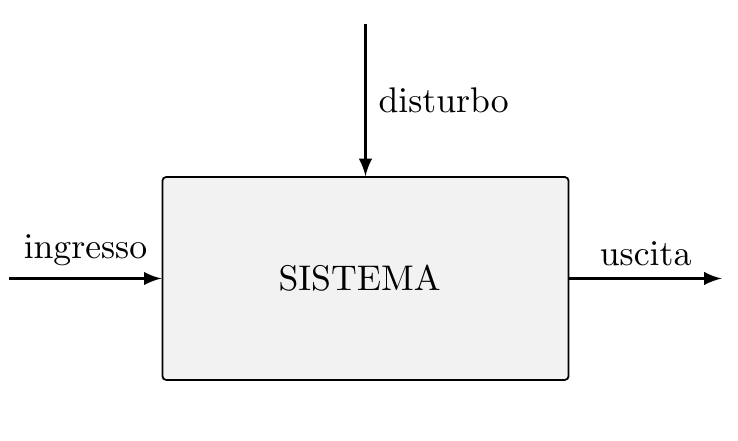
\includegraphics[scale=0.3]{Images/Schema_sistema.png}
\end{center}
Il \textbf{sistema} è un oggetto per il quale si vuole ottenere un comportamento desiderato.
\\
Esempi di sistema sono: impianto (industriale), macchinario (braccio robotico, macchina a controllo numerico, etc\dots), veicolo (auto, velivolo, drone, etc\dots), fenomeno fisico (condizioni atmosferiche), sistema biologico, sistema sociale.
\\
L'obiettivo è che l'andamento nel tempo di alcune variabili segua un segnale di riferimento.
\vspace*{0.2cm}\\
Altri elementi sono:
\begin{itemize}
    \item Controllore: unità che determina l'andamento della variabile di controllo (ingresso);
    \item Sistema di controllo: sistema (processo) + controllore;
    \item Sistemi di controllo naturali: meccanismi presenti in natura, come  quelli presenti nel corpo umano (temperatura corporea costante, ritmo cardiaco, etc\dots);
    \item Sistemi di controllo manuali: è presente l'azione dell'uomo;
    \item Sistemi di controllo automatico: uomo sostituito da un dispositivo.
\end{itemize}




\subsection{Controllo in anello aperto e anello chiuso}
Controllo in anello aperto (“feedforward”): il controllore utilizza solo il segnale di riferimento
\begin{center}
    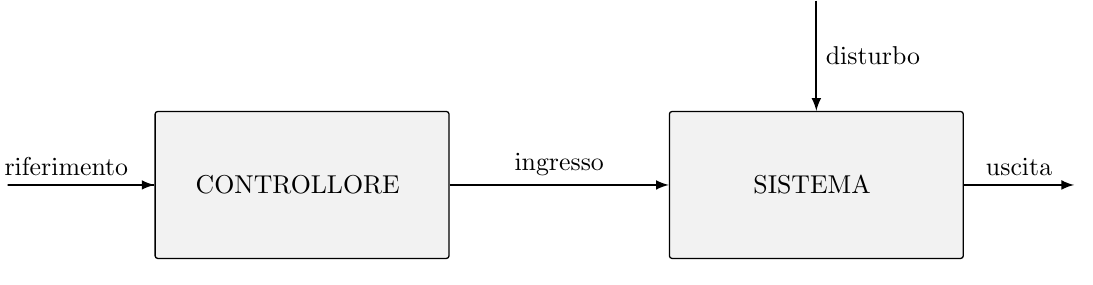
\includegraphics[scale=0.32]{Images/Anello_aperto.png}
\end{center}
Controllo in anello chiuso (“feedback” o retroazione): il controllore utilizza il segnale di riferimento e la variabile controllata ad ogni istante di tempo
\begin{center}
    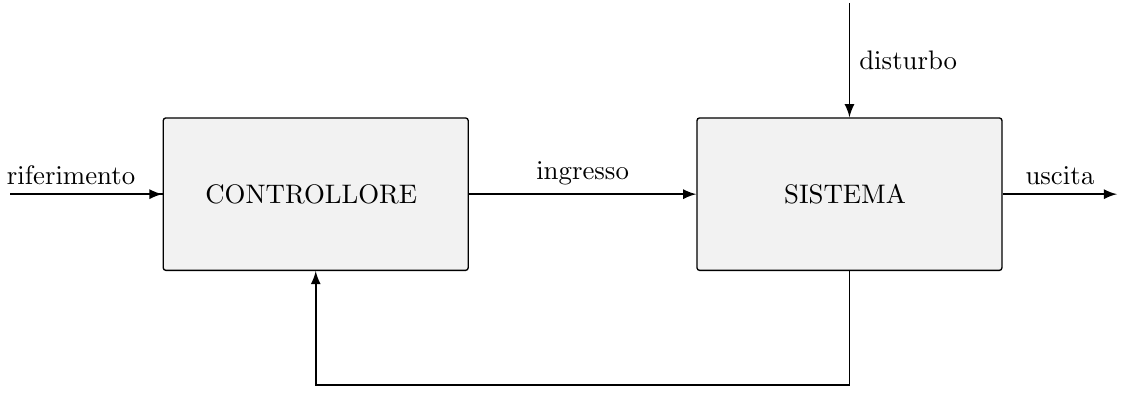
\includegraphics[scale=0.3]{Images/Anello_chiuso.png}
\end{center}
Il controllo in retroazione è un paradigma centrale nei controlli automatici.


\subsection{Progetto di un sistema di controllo}
I passi passi per progettare un sistema di controllo sono:
\begin{itemize}
    \item definizione delle specifiche: assegnazione comportamento  desiderato, qualità del controllo, costo,...
    \item modellazione del sistema (controllo e test): complessità del modello (compromesso), definizione ingressi/uscite, codifica del modello, validazione in simulazione
    \item analisi del sistema: studio proprietà “strutturali”, fattibilità specifiche
    \item sintesi legge di controllo: è basata su modello, analisi sistema controllato, stima carico computazionale
    \item simulazione sistema controllato: test su modello di controllo, test realistici (modello complesso, ritardi, quantizzazione, disturbi, ...)
    \item scelta elementi tecnologici: sensori/attuatori, elettronica di acquisizione/attuazione, dispositivo di elaborazione
    \item sperimentazione: hardware in the loop, prototipazione rapida, realizzazione prototipo definitivo
\end{itemize}





\subsection{Esempio di sistema di controllo: circuito elettrico} \label{Circuito elettrico}
\begin{center}
    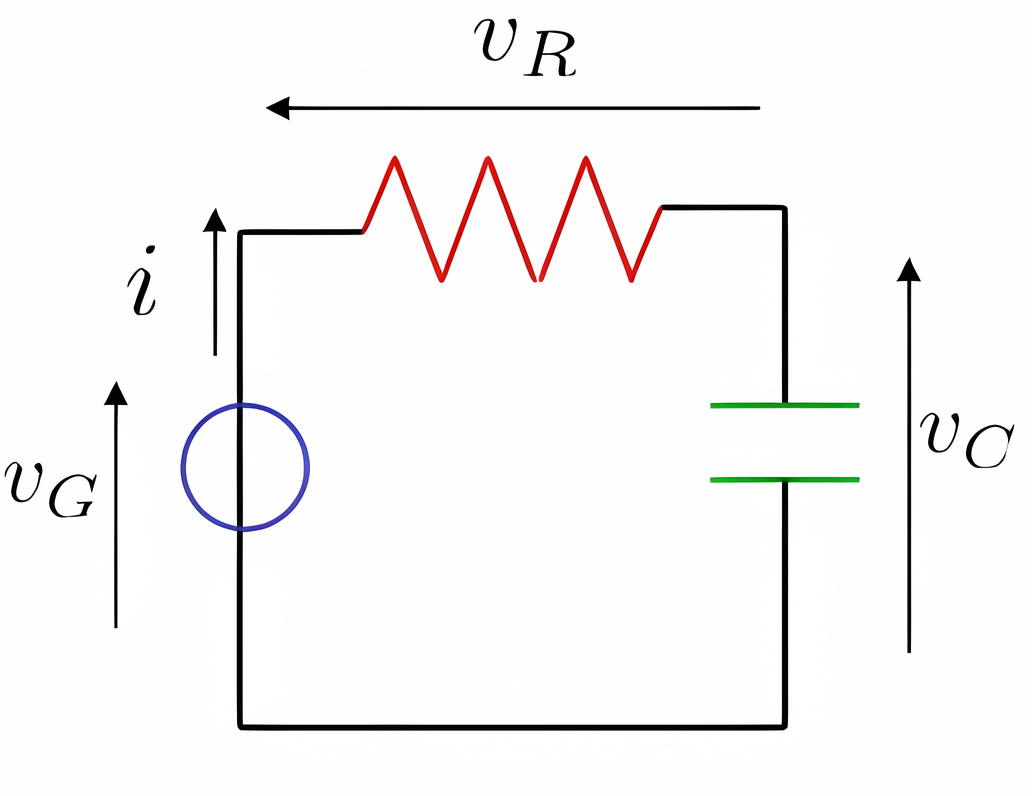
\includegraphics[scale=0.2]{Images/Es_cirucito_elettrico.png}
\end{center}
La legge che usiamo per definire il circuito (il nostro sistema) è la \textit{legge delle tensioni}
\begin{equation}
    v_R (t) = v_G (t) - v_C(t)
\end{equation} 
le leggi del condensatore e del resistore sono 
\begin{align*}
    C \cdot  \dot v_C (t) &= i(t) & v_R (t) = R\cdot i(t)
\end{align*}
Scrivendo la formula in termini di $v_C (t)$ (“stato interno”) e $v_G (t)$ (“ingresso di controllo”)
\begin{equation}
    \dot v_C (t) = \frac{1}{RC} \left(v_G (t) - v_C (t) \right)
\end{equation}




\section{Sistemi in forma di stato}
\subsection{Sistemi continui}
I \textit{sistemi continuti} sono sistemi in cui il tempo è una variabile reale: $t \in \mathbb{R}$
\begin{align*}
    \dot x(t) &= f \left( x(t), u(t), t \right) & &\text{equazione di stato}\\
    \dot y(t) &= h\left(x(t), u(t), t\right) & &\text{equazione  (trasformazione) di uscita }
\end{align*}
Definiamo inoltre $t_0$ come tempo iniziale e $x(t_0)=x_0$ come stato iniziale. \\
\textbf{N.B.} $\dot x(t) := \dfrac{d}{dt}x(t)$.
\vspace*{0.1cm}\\
Notazione:
\begin{itemize}
    \item $x(t) \in \mathbb{R}^n$ stato del sistema all'istante $t$
    \item $u(t) \in \mathbb{R}^m$ ingresso del sistema all'istante $t$
    \item $y(t) \in \mathbb{R}^p$ uscita del sistema all'istante $t$
\end{itemize}
\begin{equation}
    x(t)=
    \begin{bmatrix}
        x_1(t)\\
        ...\\
        ...\\
        ...\\
        x_n(t)
    \end{bmatrix}
    \ \ \ \ \ 
    u(t) =
    \begin{bmatrix}
        u_1(t)\\
        ...\\
        ...\\
        ...\\
        u_m(t)
    \end{bmatrix}
    \ \ \ \ \ 
    y(t) = 
    \begin{bmatrix}
        y_1(t)\\
        ...\\
        ...\\
        ...\\
        y_p(t)
    \end{bmatrix}
\end{equation}
Da notare che $x(t)$ è un vettore mentre $x_1,...,x_n$ sono scalari.\\
$x(t)$ è una variabile interna che descrive il comportamento del sistema.


\subsubsection{Equazione di stato}
L'\textit{equazione di stato} è un'equazione ordinaria (ODE) vettoriale del primo ordine (cioè l'ordine massimo delle derivate è 1)
\begin{align*}
    \dot x_1(t) &= f_1 \left(x(t), u(t), t\right)\\
    &\dots\\
    \dot x_n (t) &= f_n \left(x(t), u(t), t\right)
\end{align*}
$\mathbb{R}^n$ è detto \underline{spazio di stato}, con $n$ ordine del sistema. La funzione di stato è $f: \mathbb{R}^n \times \mathbb{R}^m \times \mathbb{R} \rightarrow \mathbb{R}^n$.
\begin{equation}
    \begin{bmatrix}
        \dot x_1(t)\\
        ...\\
        ...\\
        ...\\
        \dot x_n(t)
    \end{bmatrix} 
    =
    \begin{bmatrix}
        f_1\left(x(t),u(t),t\right)\\
        ...\\
        ...\\
        ...\\
        f_n\left(x(t),u(t),t\right)
    \end{bmatrix}
    := f\left(x(t),u(t),t\right)
\end{equation}
Avere solo derivate prime non è limitato, perché ad esempio posso inserire una prima variabile come derivata prima e una seconda variabile come derivata prima della prima variabile.

\subsubsection{Equazione di uscita}
L'equazione di uscita è un'equazione algebrica
\begin{align*}
    y_1(t) &= h_1 \left(x(t), u(t), t\right)\\
    &\dots\\
    y_p (t) &= h_p \left(x(t), u(t), t\right)
\end{align*}
$h : \mathbb{R}^n \times \mathbb{R}^m , \mathbb{R} \rightarrow R^p$ funzione di uscita
\begin{equation}
    \begin{bmatrix}
        y_1(t)\\
        ...\\
        ...\\
        ...\\
        y_p(t)
    \end{bmatrix} 
    =
    \begin{bmatrix}
        h_1\left(x(t),u(t),t\right)\\
        ...\\
        ...\\
        ...\\
        h_p\left(x(t),u(t),t\right)
    \end{bmatrix}
    := h\left(x(t),u(t),t\right)
\end{equation}
\vspace*{0.2cm}
Se la soluzione $x(t)$ a partire da un istante iniziale $t_0$ è univocamente determinata da $x(t_0)$ e $u(\tau)$ con $\tau \geq t_0$, allora il sistema è detto \textbf{causale}, cioè lo stato dipende solo da ciò che accede in passato.\\
Sotto opportune ipotesi di regolarità della funzione $f$ si dimostra esistenza e unicità della soluzione dell'equazione (differenziale) di stato (Teorema di Cauchy-Lipschitz).



\subsection{Sistemi discreti}
Nei \textit{sistemi discreti} il tempo $t$ è una variabile intera, $t \in \mathbb{Z}$.
\begin{align*}
    x(t+1) &= f \left(x(t), u(t), t\right) & &\text{equazione di stato}\\
    y(t) &= h\left(x(t), u(t), t\right) & &\text{equazione (trasformazione) di uscita}
\end{align*}
L'equazione di stato è un'equazione alle differenze finite (FDE).
\vspace*{0.2cm}\\
Notazione:
\begin{itemize}
    \item $x(t) \in \mathbb{R}^n$ stato  del sistema all'istante $t$
    \item $u(t) \in \mathbb{R}^m$ ingresso del sistema all'istante $t$
    \item $y(t) \in \mathbb{R}^p$ uscita del sistema all'istante $t$
\end{itemize}
$x(t),u(t) \text{ e } y(t)$ sono uguali ai sistemi continui.\\
Per modellare sistemi discreti nel codice basta un ciclo {\fontfamily{lmtt}\selectfont for}.



\subsection{Esempio circuito elettrico}
Riprendiamo l'esempio del \hyperlink{Circuito elettrico}{circuito elettrico}; la formula trovata è 
\begin{equation}
    \underbrace{\dot v_C(t)}_{\dot x(t)} = \frac{1}{RC} (\underbrace{v_G (t)}_{u(t)} - \underbrace{v_C (t)}_{x(t)} )
\end{equation}
In questo caso lo stato del sistema $x(t)$ è caratterizzato dalla variabile $v_C(t)$, l'ingresso dalla variabile $v_G(t)$. Supponiamo quindi di misurare (con un sensore) la tensione ai capi della resistenza, allora l'uscita del nostro sistema sarà $v_R(t)$
\begin{align*}
    \dot x(t) &= \frac{1}{RC} \left(u(t)-x(t)\right) &
    f(x,u) &= \frac{1}{RC}(u-x)
\end{align*}
da notare che in questo caso $f$ non è funzione del tempo.
\begin{equation}
    v_R(t) = v_G(t) - v_C(t) \Longrightarrow y(t) = u(t) - x(t)
\end{equation}


\subsubsection{Esempio con parametri che variano nel tempo}
Supponiamo che la resistenza sia una funzione del tempo
\begin{equation}
    R(t) = \overline{R} \left(1- \frac{1}{2} e^{-t} \right)
\end{equation}
allora 
\begin{align*}
    \dot x(t) &= \frac{1}{R(t)C} \left(u(t)-x(t)\right) &
    f(x,u,t) &= \frac{1}{R(t)C}(u-x)
\end{align*}
in questo caso $f$ è funzione del tempo.



\subsection{Esempio carrello}
\begin{center}
    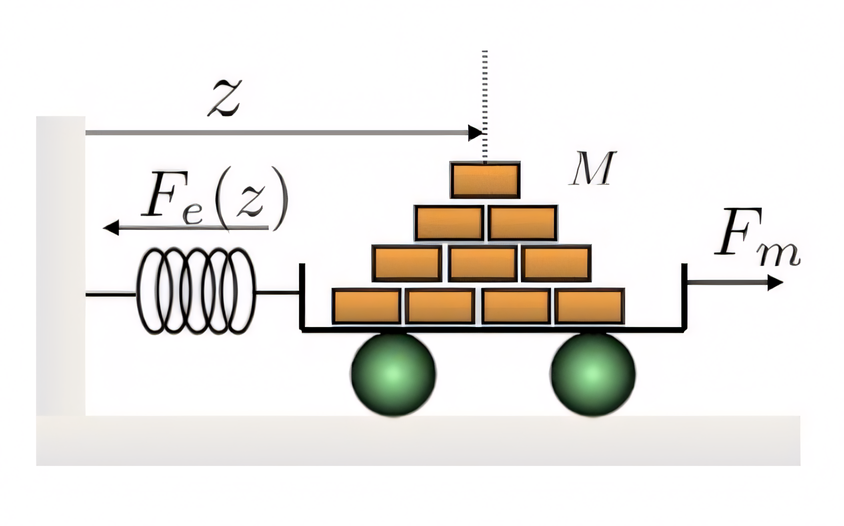
\includegraphics[scale=0.2]{Images/Es_carrello.png}
\end{center}
La legge che usiamo è la legge di Newton, prendendo $z$ come posizione del centro di massa
\begin{equation}
    M \ddot  z = -F_e + F_m
\end{equation}
con $M$ massa e $F_e$ data da
\begin{equation}
    F_e (z(t), t) = k(t)z(t)
\end{equation}
quindi la nostra equazione diventa
\begin{equation}
    M \ddot  z(t) = -k(t)z(t) + F_m(t)
\end{equation}
Siccome nella nostra formula compare una derivata seconda di una variabile ci conviene definire lo stato del sistema con la variabile stessa e la derivata prima della variabile.\\
Definiamo quindi $x_1 := z$ e $x_2:=\dot z$, con stato $x := [x_1x_2]^T$, e $u := F_m$ (ingresso).
\vspace*{0.1cm}\\
Quindi possiamo scrivere, tenendo conto che $\dot x_2(t) = \ddot z$
\begin{align*}
    \dot x_1(t) &= x_2(t)\\
    \dot x_2(t) &= -\frac{k}{M} x_1(t) + \frac{u(t)}{M}
\end{align*}
\begin{equation}
    f(x,u) = 
    \begin{bmatrix}
        f_1(x,u)\\
        f_2(x,u)
    \end{bmatrix}
    :=
    \begin{bmatrix}
        x_2\\
        -\dfrac{k}{M}x_1+\dfrac{u}{M}
    \end{bmatrix}
\end{equation}
Supponiamo di misurare $z(t)$ (sensore posizione), allora $y := z$
\begin{align*}
    \dot x_1(t) &= x_2(t)\\
    \dot x_2(t) &= -\frac{k}{M} x_1(t) + \frac{u(t)}{M}\\
    y(t) &= x_1(t)
\end{align*}
Sia $k(t) = k$ e, ricordando la formula dell'energia cinetica $E_{k}={\dfrac {1}{2}}mv^{2}$ e la formula dell'energia elastica $U={\dfrac {1}{2}}k\,\Delta x^{2}$, consideriamo come uscita l'energia totale $E_T (t) = \dfrac{1}{2} (k z^2 (t) + M \dot z^2 (t))$
\begin{align*}
    \dot x_1(t) &= x_2(t)\\
    \dot x_2(t) &= -\frac{k}{M} x_1(t) + \frac{u(t)}{M}\\
    y(t) &= \frac{1}{2} \left(k(t) x_1^2 (t) + M  x_2^2 (t)\right)
\end{align*}
quindi $h(x):= \dfrac{1}{2} (kx_1^2 + Mx_2^2)$.\\
\textbf{N.B.} Il risultato (l'uscita) vale, di solito, solo per il mio modello, in base a come l'ho impostato; nella realtà potrebbe essere diverso.


\subsection{Esempio auto in rettilineo}
\begin{center}
    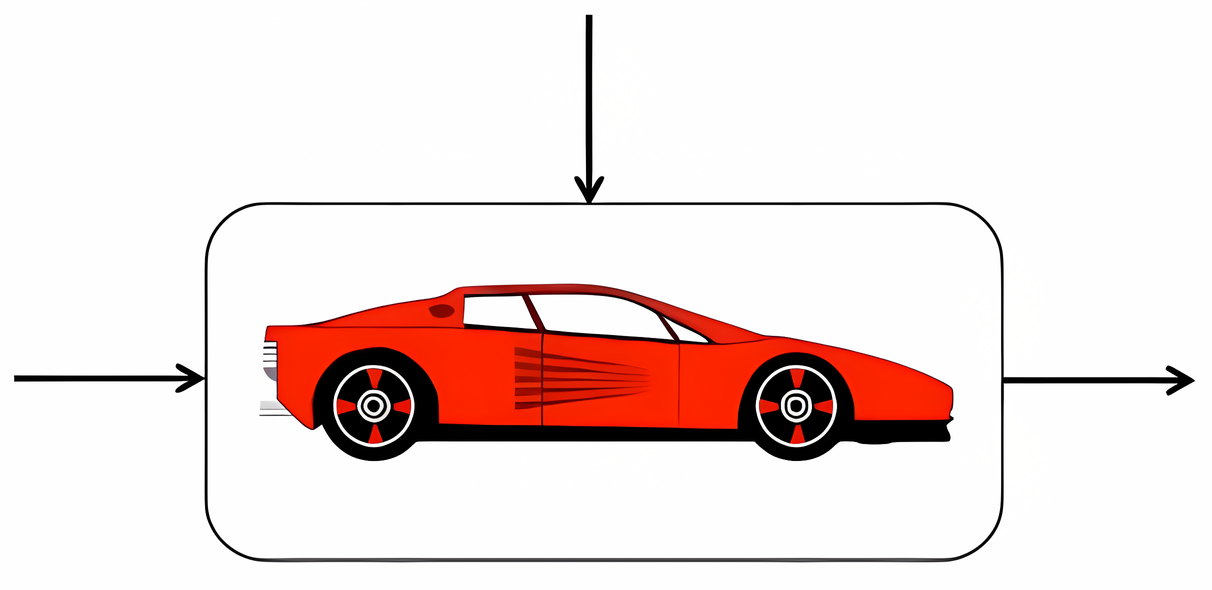
\includegraphics[scale=0.18]{Images/Es_Rettilineo.png}
\end{center}
Scriviamo la legge di Newton
\begin{equation}
    M \ddot z = F_{\text{drag}} + F_m
\end{equation}
con $M$ massa e $F_{\text{drag}}$ data da
\begin{equation}
    F_{\text{drag}} = -b \dot z
\end{equation}
Definiamo $x_1 := z$ e $x_2 := \dot z$ (stato $x := [x_1 x_2 ]^T$ ) e $u := F_m$ (ingresso). Supponiamo di misurare $z(t)$ (sensore posizione), allora $y := z$
\begin{align*}
    \dot x_1(t) &= x_2(t)\\
    \dot x_2(t) &= - \frac{b}{M} x_2(t) + \frac{1}{M}u(t)\\
    y(t) &= x_1(t)
\end{align*}
Proviamo a progettare un sistema per il \textit{cruise control}.\\
L'equazione della dinamica è
\begin{equation}
    M \ddot z(t) = -b\dot z(t) + F_m (t)
\end{equation}
Siccome siamo interessati a controllare la velocità e non la posizione, allora consideriamo come stato solo la velocità: $x := \dot z$, $u := F_m$. Supponiamo di misurare $\dot z(t)$ (sensore velocità), allora $y := x$
\begin{align*}
    \dot x(t) &= - \frac{b}{M}x(t) + \frac{1}{M}u(t)\\
    y(t) &= x(t)
\end{align*}



\subsection{Esempio pendolo}
\begin{center}
    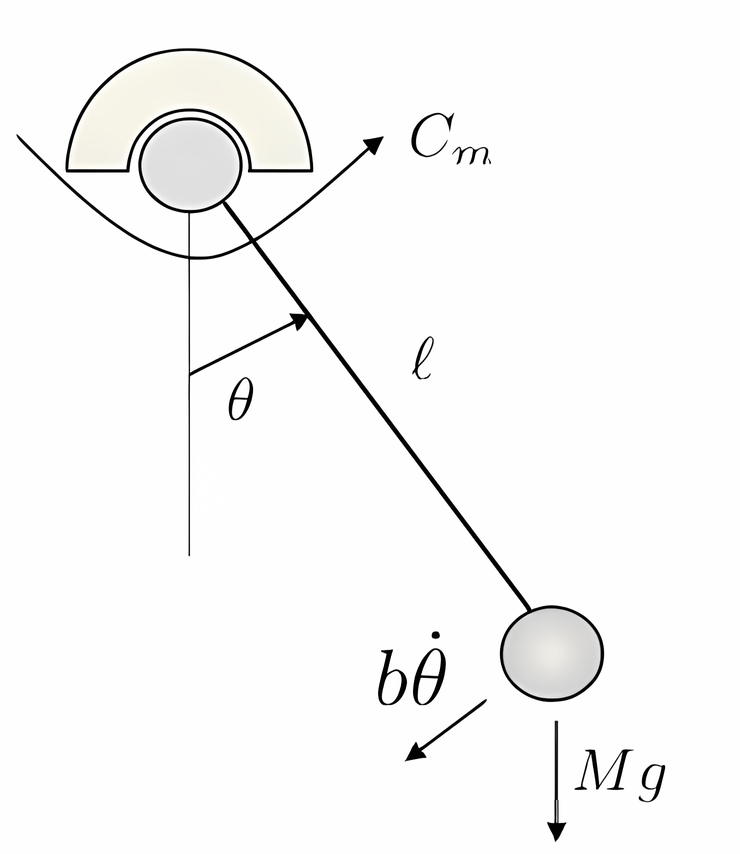
\includegraphics[scale=0.17]{Images/Es_pendolo.png}
\end{center}
Scriviamo l'equazione dei momenti
\begin{equation}
    M \ell^2 \ddot \theta= C_{\T{grav}} + C_{\T{drag}} + C_m
\end{equation}
con $M$ massa e $C_{\T{grav}}$ e $C_{\T{drag}}$ date da
\begin{align*}
    C_{\T{grav}} &=M g \ell \sin(\theta) &
    C_{\T{drag}} &= -b \dot \theta
\end{align*}
con $b$ coefficiente d'attrito.
\vspace*{0.2cm}\\
Scriviamo l'equazione della dinamica, partendo dalla formula iniziale dei momenti

\begin{equation}
    \ddot \theta(t) = -\frac{g}{\ell} \sin \left(\theta(t)\right) - \frac{b}{M \ell^2} \dot \theta(t) + \frac{1}{M \ell^2} C_m(t)
\end{equation}
Definiamo quindi $x_1 := \theta$ e $x_2 := \dot \theta$ (stato $x:= [x_1x_2]^T$) e $u := C_m$ (ingresso).\\
Supponiamo di misurare $\theta$ (sensore angolo) , allora $y := \theta$
\begin{align*}
    \dot x_1 (t) &= x_2(t)\\
    \dot x_2(t) &= -\frac{g}{\ell} \sin \left(x_1(t)\right) - \frac{b}{M \ell^2} x_2(t) + \frac{1}{M \ell^2} u(t)\\
    y(t) &= x_1(t)
\end{align*}
Se misuriamo invece la posizione verticale, allora $y := - \ell \cos(\theta)$ 
\begin{align*}
    \dot x_1 (t) &= x_2(t)\\
    \dot x_2(t) &= -\frac{g}{\ell} \sin \left(x_1(t)\right) - \frac{b}{M \ell^2} x_2(t) + \frac{1}{M \ell^2} u(t)\\
    y(t) &= - \ell \cos(\theta)
\end{align*}



\subsection{Traiettoria di un sistema}
Dato un istante iniziale $t_0$ e uno stato iniziale $x_{t_0}$, la funzione del tempo $(x(t), u(t)), \ t>t_0$, che soddisfa l'equazione di stato $\dot x(t) = f (x(t), u(t), t)$ si dice traiettoria (movimento) del sistema. In particolare, $x(t)$ si dice traiettoria dello stato. Consistentemente, $y(t)$ si dice traiettoria dell'uscita.
\vspace*{0.2cm}\\
\textbf{N.B.} per sistemi senza ingresso (quindi non forzati) la traiettoria dello stato $x(t), \ t>t_0$ è determinata solo dallo stato iniziale $x_{t_0}$.


\subsubsection{Esempio}
Definiamo un sistema con stato $x$ e stato iniziale $x_0$
\begin{align*}
    x &:=
    \begin{bmatrix}
        x_1\\
        x_2
    \end{bmatrix}
    &
    x_0 &:=
    \begin{bmatrix}
        5\\
        3
    \end{bmatrix}
    &
    t_0 &= 0
\end{align*}
\begin{align*}
    \dot x_1(t) &= x_2(t)\\
    \dot x_2(t) &= u(t)
\end{align*}
Assegno a $x_1$, $x_2$ e $u(t)$ le seguenti equazioni
\begin{align*}
    \overline{x_1}(t) &= 5+3t+t^2\\
    \overline{x_2}(t) &= 3+2t\\
    \overline{u}(t) &= 2
\end{align*}
Se le equazioni di $\overline{x_1}$ e $\overline{x_2}$ soddisfano le condizioni iniziali e la funzione di stato ($\dot x_1$ e $\dot x_2$) allora quelle equazioni sono la traiettoria del sistema.\\
Infatti
\begin{equation}
    \overline{x_0} = 
    \begin{bmatrix}
        5+3t+t^2\\
        3+2t
    \end{bmatrix}_{t=0} 
    =
    \begin{bmatrix}
        5\\
        3
    \end{bmatrix}
\end{equation}
\begin{align*}
    &\overline{x_0} = 
    \begin{bmatrix}
        5+3t+t^2\\
        3+2t
    \end{bmatrix}_{t=0} 
    =
    \begin{bmatrix}
        5\\
        3
    \end{bmatrix}
    &
    \frac{d}{dt} 
    \begin{bmatrix}
        5+3t+t^2\\
        3+2t
    \end{bmatrix}
    =
    \begin{bmatrix}
        3+2t\\
        2
    \end{bmatrix}
\end{align*}



\subsection{Equilibrio di un sistema}
Dato un sistema (non forzato) $\dot x(t) = f (x(t), t)$, uno stato $x_e$ si dice \textit{equilibrio del sistema} se $x(t) = x_e$ , $t\geq t_0$ è una traiettoria del sistema.
\vspace*{0.2cm}\\
Dato un sistema (forzato) $\dot x(t) = f (x(t), u(t), t)$, $(x_e , u_e )$ si dice \textit{coppia di equilibrio} del sistema se $(x(t), u(t)) = (x_e , u_e )$, $t \geq t_0$ , è una traiettoria del sistema.
\vspace*{0.2cm}\\
Per un sistema (tempo invariante continuo) $\dot x(t) = f (x(t), u(t))$ data una coppia di equilibrio $(x_e,u_e)$ vale $f(x_e,u_e)=0$.\\
Se il sistema è non forzato, dato un equilibrio $x_e$ vale $f(x_e)=0$.


\subsubsection{Esempio pendolo}
\begin{align*}
    \dot x_1(t) &= x_2(t) &= f_1(x(t),u(t))\\
    \dot x_2(t) &= - \frac{G}{\ell} \sin (x_1(t)) - \frac{b}{M \ell ^2}x_2(t) + \frac{1}{M\ell^2}u(t) &=f_2(x(t),u(t))
\end{align*}
Siccome sappiamo che, data una coppia di equilibrio $(x_e,u_e)$, vale $f(x_e,u_e)=0$, allora per trovare l'equilibrio del pendolo imponiamo 
\begin{equation}
    f(x_e,u_e)=0
\end{equation}
cioè:
\begin{equation}
    \begin{cases}
        x_{2e}(t) = 0\\
        \\
        - \dfrac{G}{\ell} \sin (x_{1e}) - \dfrac{b x_{2e}}{M \ell ^2} + \dfrac{1}{M\ell^2}u_e =0
    \end{cases}
\end{equation}
sostituendo $x_{2e}(t)=0$ nell'ultima equazione
\begin{equation}
    - \dfrac{G}{\ell} \sin (x_{1e}) + \dfrac{1}{M\ell^2}u_e =0 \Longrightarrow u_e = M G \ell \sin(x_{1e})
\end{equation}
In conclusione, le coppie di equilibrio del sistemo sono tutti fli $(x_{1e}, x_{2e},u_e)$ che soddisfano
\begin{equation}
    \begin{cases}
        u_e = M G \ell \sin(x_{1e})\\
        x_{2e}=0
    \end{cases}
\end{equation}




\subsection{Classificazione dei sistemi in forma di stato}
La classe generale è  $x \in \mathbb{R}^n , u \in \mathbb{R}^m , y\in \mathbb{R}^p$
\begin{align*}
    \dot x(t) &= f (x(t), u(t), t) & &\T{equazione di stato}\\
    y(t) &= h(x(t), u(t), t) & &\T{equazione di uscita}  
\end{align*}
\begin{itemize}
    \item I sistemi \textbf{monovariabili} (SISO, Single Input Single Output) sono una sottoclasse di sistemi \textbf{multivariabili} (MIMO, Multiple Input Multiple Output); sono tali se $m=p=1$, altrimenti sono dei sistemi MIMO;
    \item I sistemi \textbf{strettamente propri} sono una sotto classe dei \textbf{sistemi propri}; sono tali se $y(t) = h(x(t),t))$, quindi se l'uscita dipende esclusivamente dall'ingresso, chiamati quindi sistemi causali (tutti i sistemi che abbiamo visto fin'ora sono sistemi propri).
    \item I sistemi \textbf{non forzati} sono una sotto classe dei \textbf{sistemi forzati}; un esempio di sistema non forzato è il seguente
    \begin{align*}
        \dot x(t) &= f(x(t),t)\\
        y(t) &= h(x(t),t)
    \end{align*}
    \item I sistemi \textbf{tempo invarianti} sono una sotto classe di sistemi \textbf{tempo  varianti}.\\
    I tempo invarianti sono tali se, data una traiettoria $ (x(t), u(t)), t\geq t_0$, con $x(t_0)=x_0$, per ogni $\Delta \in \mathbb{R}$ vale che $x(t_0+\Delta)=x_0$ allora $(x_{\Delta} (t), u_{\Delta} (t)) = (x(t-\Delta), u(t-\Delta))$ è una traiettoria.\\
    Si può dimostrare che sistemi tempo invarianti sono del tipo
    \begin{align*}
        \dot x(t) &= f (x(t), u(t)) &x(0)=x_0\\
        y(t) &= h(x(t), u(t))
    \end{align*}
    e senza senza perdita di generalità possiamo scegliere $t_0=0$.\\
    Graficamente:
    \begin{center}
        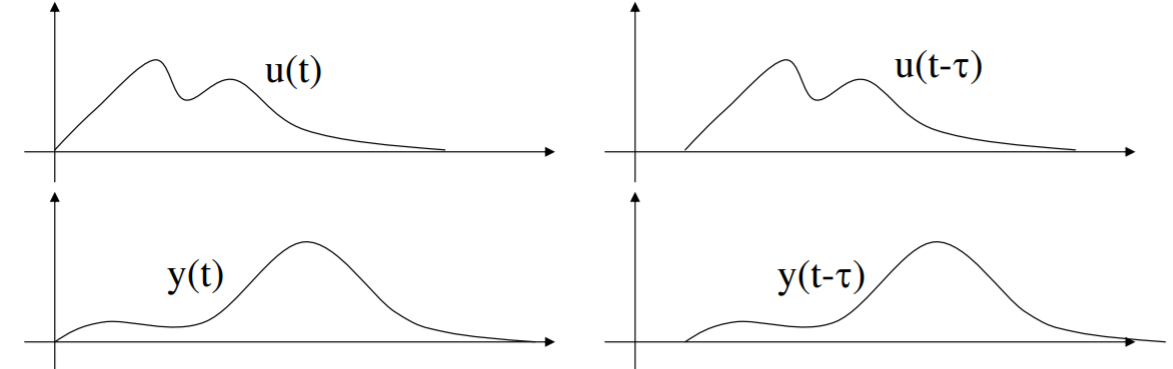
\includegraphics[scale=0.3]{Images/Sistemi_tempo_invarianti.png}
    \end{center}
    \item I \textbf{sistemi lineari} sono una sotto classe di \textbf{sistemi non lineari}.\\
    I sistemi lineari sono tali se le funzioni di stato e di uscita sono lineari in $x$ e $u$:
    \begin{align*}
        \dot x_1 (t) &= a_{11} (t)x_1 (t) + a_{12} (t)x_2 (t) + . . . + a_{1n} (t)x_n (t)+ b_{11} (t)u_1 (t) + b_{12} (t)u_2 (t) + . . . + b_{1m} (t)u_m (t)\\
        \dot x_2 (t) &= a_{21} (t)x_1 (t) + a_{22} (t)x_2 (t) + . . . + a_{2n} (t)x_n (t)+ b_{21} (t)u_1 (t) + b_{22} (t)u_2 (t) + . . . + b_{2m} (t)u_m (t)\\
        ...\\
        ...\\
        ...\\
        \dot x_n (t) &= a_{n1} (t)x_1 (t) + a_{n2} (t)x_2 (t) + . . . + a_{nn} (t)x_n (t)+ b_{n1} (t)u_1 (t) + b_{n2} (t)u_2 (t) + . . . + b_{nm} (t)u_m (t)
    \end{align*}
    per $y(t)$ invece 
    \begin{align*}
        y_1 (t) &= c_{11} (t)x1 (t) + c_{12} (t)x_2 (t) + . . . + c_{1n} (t)x_n (t)+ d_{11} (t)u_1 (t) + d_{12} (t)u_2 (t) + . . . + d_{1m} (t)u_m (t)\\
        y_2 (t) &= c_{21} (t)x_1 (t) + c_{22} (t)x_2 (t) + . . . + c_{2n} (t)x_n (t)+ d_{21} (t)u_1 (t) + d_{22} (t)u_2 (t) + . . . + d_{2m} (t)u_m (t)\\
        ...\\
        ...\\
        ...\\
        y_p (t) &= c_{p1} (t)x_1 (t) + c_{p2} (t)x_2 (t) + . . . + c_{pn} (t)x_n (t)+ d_{p1}(t)u_1 (t) + d_{p2} (t)u_2 (t) + . . . + d_{pm} (t)u_m (t)
    \end{align*}
\end{itemize}



\subsection{Proprietà dei sistemi lineari}
\subsubsection{Sistemi lineri in forma matriciale}
Definiamo le matrici $A(t) \in \mathbb{R}^{n \times n} , B(t) \in \mathbb{R}^{n \times m} , C(t) \in \mathbb{R}^{p \times n} , D(t) \in \mathbb{R}^{p \times m}$
\begin{align*}
    A(t) &= \begin{bmatrix}
        a_{11}(t) & ... & a_{1n}(t)\\
        .\\
        .\\
        a_{n1}(t) & ... & a_{nn}(t)
    \end{bmatrix}
    &
    B(t) &= \begin{bmatrix}
        b_{11}(t) & ... & b_{1m}(t)\\
        .\\
        .\\
        b_{n1}(t) & ... & b_{nm}(t)
    \end{bmatrix}\\
    C(t) &= \begin{bmatrix}
        c_{11}(t) & ... & c_{1n}(t)\\
        .\\
        .\\
        c_{p1}(t) & ... & c_{pn}(t)
    \end{bmatrix}
    &
    D(t) &= \begin{bmatrix}
        d_{11}(t) & ... & d_{1m}(t)\\
        .\\
        .\\
        d_{pn1}(t) & ... & d_{pm}(t)
    \end{bmatrix}
\end{align*}
quindi scriviamo
\begin{equation}
    \begin{bmatrix}
        \dot x_1(t)\\
        .\\
        .\\
        \dot x_n(t)
    \end{bmatrix}
    = A(t)
    \begin{bmatrix}
        x_1(t)\\
        .\\
        .\\
        x_n(t)
    \end{bmatrix}
    + B(t)
    \begin{bmatrix}
        u_1(t)\\
        .\\
        .\\
        u_m(t)
    \end{bmatrix}
\end{equation}
che equivale a 
\begin{align*}
    \dot x(t) &= A(t) x(t) + B(t) u(t)\\
    y(t) &= C(t)x(t) + D(t) u(t)
\end{align*}


\subsection{Sistemi lineari tempo-invarianti}
\begin{align*}
    \dot x(t) = A x(t) + B u(t)\\
    y(t) = C x(t) + D u(t)
\end{align*}
con $A,B,C,D$ matrici costanti.


\subsubsection{Esempio carrello}
\begin{center}
    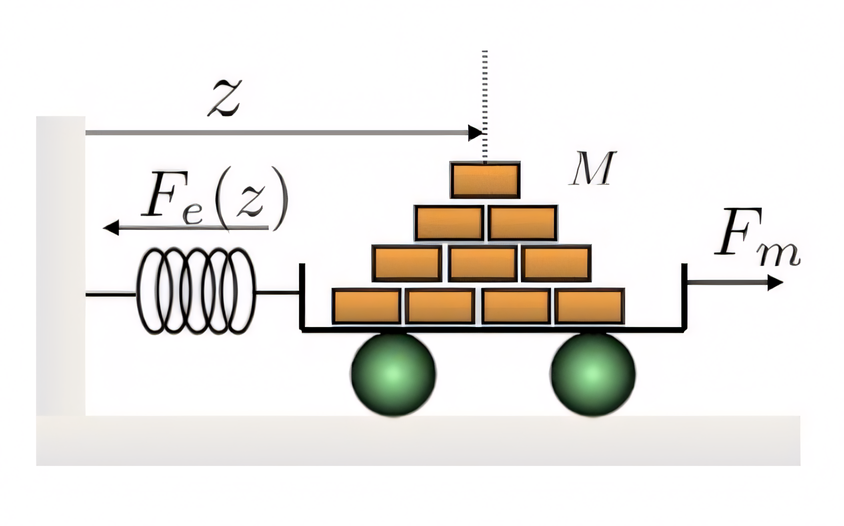
\includegraphics[scale=0.2]{Images/Es_carrello.png}
\end{center}
\begin{align*}
    \dot x_1(t) &= x_2(t) & f_1(x,u,t) &= x_2\\
    \dot x_2(t) &= - \frac{k(t)}{M}x_1(t) + \frac{1}{M} u(t) & f_2(x,u,t) &= - \frac{k(t)}{M}x_1 + \frac{1}{M}u\\
    y(t) &= x_1(t)
\end{align*}
$f_2$ dipende esplicitamente da $t$ attraverso $k(t)$ quindi è un sistema tempo \underline{variante}. Se $k(t) = \overline{k}$ per ogni $t$ allora tempo \underline{invariante}.\\
Siccome $f_1$ e $f_2$ dipendono linearmente da $x$ e $u$ il sistema è \underline{lineare}. (Se $k(t) = \overline{k}$ il sistema è \underline{lineare tempo invariante}.)
\begin{align*}
    \begin{bmatrix}
        \dot x_1(t)\\
        \dot x_2(t)
    \end{bmatrix}
    &=
    \underbrace{\begin{bmatrix}
        0 & 1\\
        -\frac{k(t)}{M} & 0
    \end{bmatrix}}_{A}
    \begin{bmatrix}
        x_1(t)\\
        x_2(t)
    \end{bmatrix}
    +
    \underbrace{\begin{bmatrix}
        0\\
        \frac{1}{M}
    \end{bmatrix}}_{B}
    u(t)
    \\
    y(t) &= 
    \underbrace{\begin{bmatrix}
        1 & 0
    \end{bmatrix}}_{C}
    \begin{bmatrix}
        x_1(t)\\
        x_2(t)
    \end{bmatrix}
    + \underbrace{0}_D u(t)
\end{align*}
per $k$ costante:
\begin{align*}
    A &= \begin{bmatrix}
        0 & 1\\
        - \frac{k}{M} & 0
    \end{bmatrix}
    &
    B &= 
    \begin{bmatrix}
        0\\
        1
    \end{bmatrix}
    &
    C &= 
    \begin{bmatrix}
        1 & 0
    \end{bmatrix}
\end{align*}


\subsubsection{Sistemi lineari tempo-invarianti SISO}
I sistemi lineari tempo-invarianti single input single output (SISO) sono caratterizzati dalle matrici $A \in \mathbb{R}^{n \times n} , B \in \mathbb{R}^{n \times 1}, C \in \mathbb{R}^{1 \times n} , D \in \mathbb{R}^{1 \times 1}$, ovvero $B$ è un vettore, $C$ è un vettore riga e $D$ è uno scalare.


\subsection{Principio di sovrapposizione degli effetti}
Prendiamo un sistema lineare (anche tempo-variante)
\begin{align*}
    \dot x(t) &= A(t)x(t) + B(t)u(t)\\
    y(t) &= C(t)x(t) + D(t)u(t)
\end{align*}
Sia $(x_a (t), u_a (t))$ traiettoria con $x_a (t_0)$ = $x_{0a}$.\\
Sia $(x_b (t), u_b (t))$ traiettoria con $x_b (t_0)$ = $x_{0b}$.
\vspace*{0.1cm}\\
Allora $\forall \alpha, \beta \in \mathbb{R}$ dato lo stato iniziale $x_{ab}(t_0) = \alpha x_{0a}+\beta x_{0b}$, si ha che
\begin{equation}
    (x_{ab}(t), u_{ab}(t)) = (\alpha x_{a}(t) + \beta x_b(t), \alpha u_a(t)+\beta u_b(t))
\end{equation}
è traiettoria del sistema, ovvero applicando come ingresso $u_{ab}=\alpha u_a(t) + \beta u_b(t)$ la traiettoria di stato è $x_{ab} (t) = \alpha x_a (t) + \beta x_b (t)$
\begin{equation}
    \begin{rcases}
        \alpha x_{0a}(t)+\beta x_{0b}(t)\\
        \alpha u_a(t) + \beta u_b(t)(t)
    \end{rcases}
    \Longrightarrow
    \alpha x_a(t) + \beta x_b(t)
\end{equation}
\vspace*{0.2cm}
\textbf{IMPORTANTE:} non vale per i sistemi non lineari.

\subsubsection*{Dimostrazione}
Per dimostrarlo dobbiamo provare che soddisfa l'equazione differenziale
\begin{align*}
    \frac{d}{dt}x_{ab}(t) &= \alpha \dot x_a(t) + \beta \dot x_b(t)\\
    &= \alpha(A(t)x_a (t) + B(t)u_a (t)) + \beta (A(t)x_b (t) + B(t)u_b (t))\\
    &= A(t)(\alpha x_a (t) + \beta x_b (t)) + B(t)( \alpha u_a (t) + u_b (t))
\end{align*}
Per sistemi lineari sotto opportune ipotesi su $A(t)$ e $B(t)$ si può dimostrare che la soluzione è unica.\\
Si dimostra lo stesso anche per l'uscita.


\subsection{Evoluzione libera e evoluzione forzata}
Sfruttando il principio di sovrapposizione degli effetti prendiamo due sistemi \circled{A} e \circled{B} 
\begin{align*}
   \circled{A} \ x(t_0) &= x_0 =x_{0a} {\color{violet} \neq 0} & \circled{B} \ \ \ x_{0b}&=0\\
    u_a(t) &= 0 \ \ \forall t \geq t_0 & u_b(t) &= u(t) {\color{violet}\neq 0}
\end{align*}
chiamiamo $x_a(t)=x_\ell(t)$ e $x_b(t) = x_f(t)$
\begin{align*}
    \alpha x_{0a} + \beta x_{0b} &= \underbrace{\alpha}_{1} x_0 = x_0 & 
    \alpha u_a(t) + \beta u_b(t) &= \underbrace{\beta}_{1}u(t) = u(t)
\end{align*}
quindi
\begin{equation}
    x_{ab}(t) = \underbrace{x_\ell(t)}_{\substack{\text{evoluzione} \\ \text{libera}}} + \underbrace{x_f(t)}_{\substack{\text{evoluzione} \\ \text{forzata}}}
\end{equation}
L'\textbf{evoluzione libera} è definita come $x_\ell(t)$ per $t \geq t_0$, tale che $x_\ell (t_0)=x_0$ e $u_l(t)=0$ per $t \geq t_0$, e uscita $y_\ell(t)=C(t)x_\ell(t)$.\\
L'\textbf{evoluzione forzata} è definita come $x_f(t)$ per $t \geq t_0$, tale che $x_f (t_0)=0$ e $u_l(t)=u(t)$ per $t \geq t_0$, e uscita $y_f(t)=C(t)x_f(t)+D(t)u(t)$.
\vspace*{0.2cm}\\
\textbf{IMPORTANTE:} non vale per i sistemi non lineari.


\subsubsection{Traiettorie di un sistema LTI: esempio scalare}
Definiamo un sistema lineare tempo invariante (LTI) scalare $x \in \mathbb{R}$, $u \in \mathbb{R}$, $y \in \mathbb{R}$
\begin{align*}
    \dot x(t) &= ax(t) + bu(t) &x(0) = x_0\\
    y(t) &= cx(t) + du(t)
\end{align*}
dall'analisi matematica possiamo scrivere il sistema come soluzione omogenea + soluzione particolare
\begin{align*}
    x(t) &= e^{at}x_0 + \int_0^t e^{a(t-\tau)}bu(\tau) d \tau \\
    y(t) &= ce^{at}x_0 + c \int_0^t e^{a(t-\tau)}bu(\tau) d \tau + du(t)
\end{align*}
ricordiamo che la funzione esponenziale si può scrivere come
\begin{equation}
    e^{at} = 1 + at + \frac{(at)^2}{2!} + \frac{(at)^3}{3!} + ...
\end{equation}


\subsubsection{Traiettorie di un sistema LTI: caso generale}
Definiamo un sistema lineare tempo invariante (LTI) $x\in \mathbb{R}^n, u\in \mathbb{R}^m, y\in \mathbb{R}^p$
\begin{align*}
    \dot x(t) &= Ax(t) + Bu(t) &x(0) = x_0\\
    y(t) &= Cx(t) + Du(t)
\end{align*}
\begin{align*}
    \underbrace{x(t)}_{\mathbb{R}^n} &= \underbrace{e^{At}}_{\mathbb{R}^{n \times n}} \underbrace{x_0}_{\mathbb{R}^n} + \int_0^t e^{A(t-\tau)}Bu(\tau) d \tau \\
    y(t) &= Ce^{at}x_0 + c \int_0^t e^{A(t-\tau)}Bu(\tau) d \tau + Du(t)
\end{align*}

Ricordiamo che l'esponenziale di matrice si può scrivere come
\begin{equation}
    e^{At} = I + At + \frac{(At)^2}{2!} + \frac{(At)^3}{3!} + ...
\end{equation}
\begin{equation}
    x(t) = \underbrace{e^{At} x_0}_{\substack{\text{evoluzione} \\ \text{libera}}} + \underbrace{\int_0^t e^{A(t-\tau)}Bu(\tau) d \tau}_{\substack{\text{evoluzione} \\ \text{forzata}}}
\end{equation}
\begin{align*}
    x_\ell(t) &= e^{At}x_0 & x_f(t) &= \int_0^t e^{A(t-\tau)}Bu(\tau) d \tau
\end{align*}


\subsubsection{Esempio sistema non forzato}
\begin{align*}
    \dot x_1(t) = \lambda_1 x_1(t) & \dot x_1(t) = \lambda_2 x_2(t)
\end{align*}
\begin{equation}
    \begin{bmatrix}
        \dot x_1(t)\\
        \dot x_2(t)
    \end{bmatrix}
    =
    \underbrace{\begin{bmatrix}
        \lambda_1 & 0\\
        0 & \lambda_2  
    \end{bmatrix}}_{A}
    \begin{bmatrix}
        x_1(t)\\
        x_2(t)
    \end{bmatrix}
\end{equation}
$A := \Lambda$ matrice diagonale.
\vspace*{0.2cm}\\
Il nostro è un sistema non forzato, quindi c'è solo l'evoluzione libera:
\begin{equation}
    x(t) = e^{\Lambda t}x_0
\end{equation}
\begin{align*}
    e^{\Lambda t} &= 
    \begin{bmatrix}
        1 & 0\\
        0 & 1
    \end{bmatrix}
    +
    \begin{bmatrix}
        \lambda_1 & 0\\
        0 & \lambda_2
    \end{bmatrix}
    +
    \begin{bmatrix}
        \lambda_1 & 0\\
        0 & \lambda_2
    \end{bmatrix}^2 \frac{t^2}{2!} + ...\\
    &=\begin{bmatrix}
        1 & 0\\
        0 & 1
    \end{bmatrix}
    +
    \begin{bmatrix}
        \lambda_1 & 0\\
        0 & \lambda_2
    \end{bmatrix}
    +
    \begin{bmatrix}
        \frac{\lambda_1^2 t^2}{2!} & 0\\
        0 & \frac{\lambda_2^2 t^2}{2!}
    \end{bmatrix} + ...\\
    e^{at} = 1 + at + \frac{(at)^2}{2!} + \frac{(at)^3}{3!} + ... \Longrightarrow&=
    \begin{bmatrix}
        e^{\lambda_1 t} & 0\\
        0 & e^{\lambda_2 t}
    \end{bmatrix}
\end{align*}
Quindi nel caso generale di $\Lambda \in \mathbb{R}^{n \times n}$
\begin{equation}
    e^{\Lambda t} = 
    \begin{bmatrix}
        e^{\lambda_1 t} & 0 & ... & 0\\
        0 & e^{\lambda_2 t} & ... & 0\\
        .\\
        .\\
        0 & ... & 0 & e^{\lambda_n t}
    \end{bmatrix}
\end{equation}


\subsubsection{Proprietà della matrice esponenziale} \label{proprietà della matrice esponenziale}
Esponenziale e cambio di base:
\begin{equation}
    e^{TAT^{-1}} = Te^{At}T^{-1}
\end{equation}
Data una matrice $A \in \mathbb{R}^{n \times n}$, esiste $J$ matrice diagonale a blocchi, chiamata \textit{matrice di Jordan}, che è unica a meno di permutazioni dei blocchi, tale che
\begin{equation}
    A = T^{-1} J T
\end{equation}
con $T$ matrice invertibile (matrice del cambio base). Questa formula viene chiamata \textit{forma di Jordan}.
\vspace*{0.2cm}\\
La matrice di Jordan è fatta in questo modo
\begin{center}
    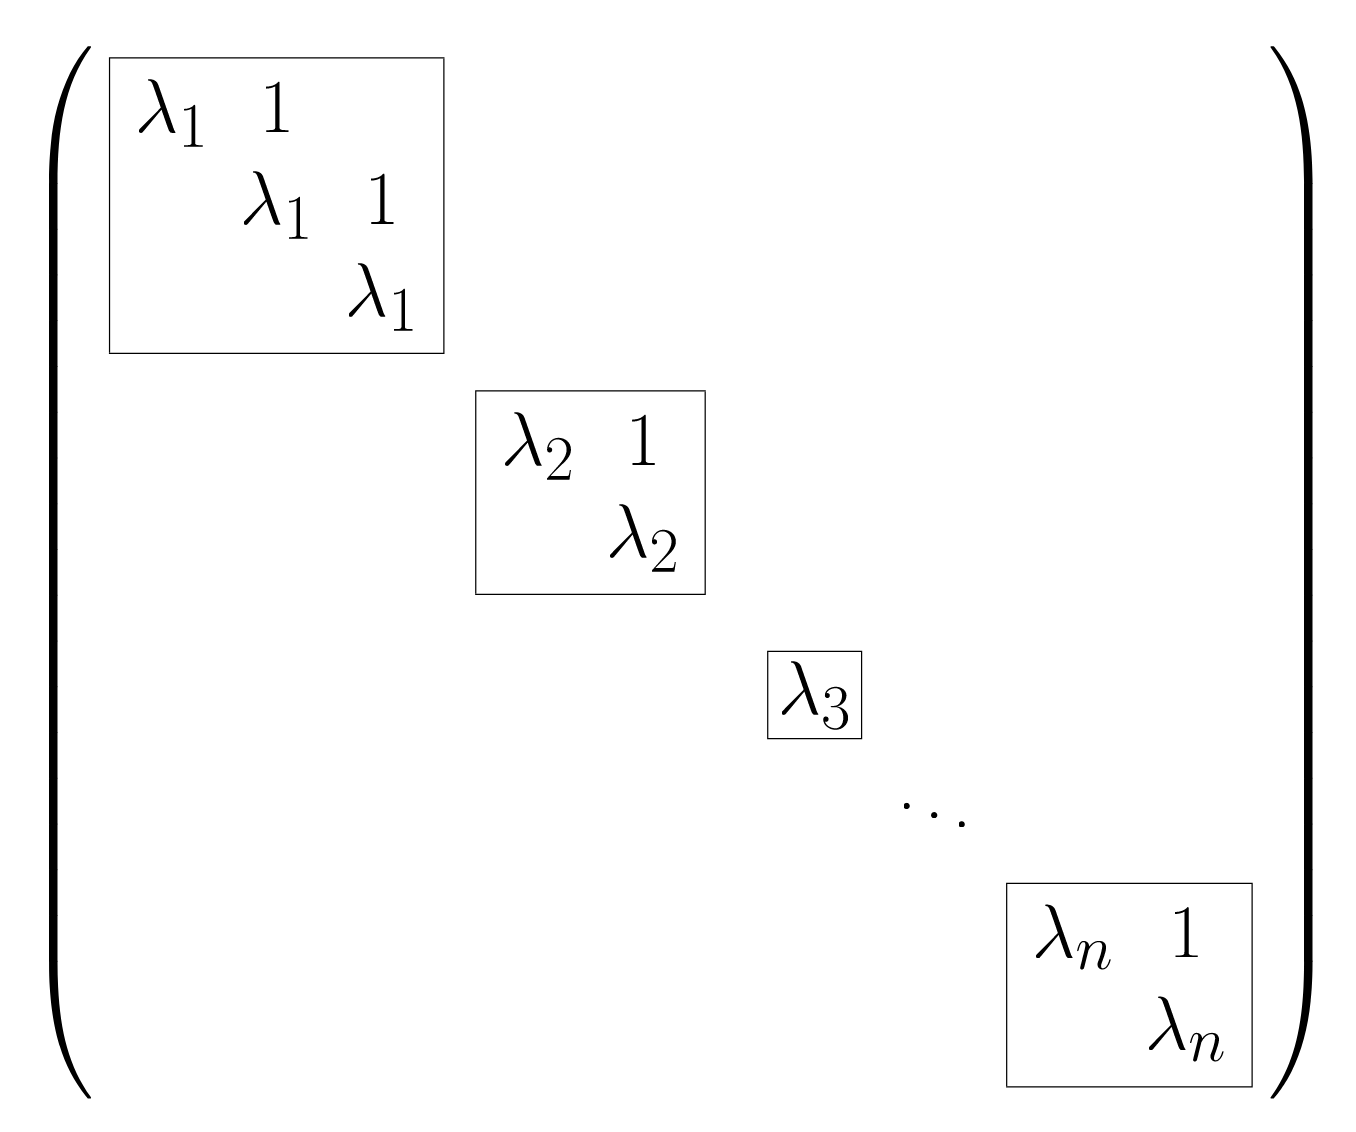
\includegraphics[scale=0.13]{Images/Jordan_matrix.png}
\end{center}
con $\lambda_i$ autovalore di $A$.
\vspace*{0.2cm}\\
Utilizzando questa forma riconduco il calcolo di $e^{At}$ al calcolo di 
\begin{equation}
    e^{
        \begin{bmatrix} 
            \lambda & 1 & 0 & ... & 0\\
            0 & ... & ... & ... &0\\
            ... & ... & ... & ... & 0\\
            ... & ... & ... & ... & 1\\
            0 & ... & ... & 0 & \lambda
        \end{bmatrix}
        }
        = e^{\lambda t}
        \begin{bmatrix}
            1 & t & \frac{t^2}{2!} & ... \\
            0 & 1 & t & \frac{t^2}{2!} & ... \\
            ... & ... & ... & ... & ...\\
            0 & ... & ... & ... & 1
        \end{bmatrix}
\end{equation}
\textbf{IMPORTANTE:} tutti gli elementi di $e^{At}$ sono del tipo
\begin{equation}
    t^qe^{\lambda t}
\end{equation}
con $q$ intero e $\lambda_i$ autovalori di A


\subsection{Rappresentazioni equivalenti}
Effettuiamo un cambio di base mediante una matrice $T$
\begin{equation}
    \hat x(t) = T x(t)
\end{equation}
ed essendo $T$ invertibile
\begin{equation}
    x(t) = T^{-1} \hat x(t)
\end{equation}
Sostituendo nell'equazione della dinamica si ottiene
\begin{align*}
    {\color{violet} T \cdot} \underbrace{T^{-1} \dot{\hat x}(t)}_{\dot x(t)} &= A \underbrace{T^{-1} \hat x(t)}_{x(t)} + B u(t) {\color{violet} \cdot T } \\
\end{align*}
\begin{align*}
    \dot{\hat x}(t) &= TAT^{-1} \hat x(t) + T B u(t)\\
    y(t) &= CT^{-1} \hat x(t) + D u(t)
\end{align*}
Allora chiamo $\hat A = TAT^{-1}, \hat B=TB, \hat C = CT^{-1}, \hat D = D$
\begin{align*}
    \dot{\hat x}(t)  &= \hat A \hat x(t) + \hat B u(t)\\
    y(t) &= \hat C \hat x(t) + \hat D u(t)
\end{align*}
se $T$ è una matrice tale che
\begin{equation}
    J = TAT^{-1}
\end{equation}
allora
\begin{equation}
    \dot{\hat x} = J \hat x(t) + T B u(t)
\end{equation}
\begin{align*}
    \hat x_\ell (t) = e^{JT} \hat x_0 = T^{-1} e^{Jt}T x_0
\end{align*}




\subsection{Modi di un sistema lineare tempo invariante}
Prendiamo un sistema lineare tempo invariante con $x \in \mathbb{R}^n, u \in \mathbb{R}^m, y \in \mathbb{R}^p$ e $x(0)=x_0$
\begin{align*}
    \dot x(t) &= A x(t) + B u(t)\\
    y(t) &= C x(t) + D u(t)
\end{align*}
Indichiamo con $\lambda_1,...,\lambda_r$ gli $r \leq n$ autovalori (reali o complessi coniugati) distinti della matrice $A$, con molteplicità algebrica $n_1,...,n_r \geq 0$ tali che $\sum\limits ^r_{i=1} n_i = n$.\\
Le componenti dell'evoluzione libera dello stato $x_\ell(t)$ si possono scrivere come
\begin{equation}
    x_{\ell,j} = \sum^r_{i=1}\sum^{h_i}_{q=1} \gamma_{jiq}t_{q-1}e^{\lambda_i t} \tag*{$j=1,...,n$}
\end{equation}
per opportuni valori di $h_i \leq n_i$, dove i coefficienti $\gamma_{jiq}$ dipendono dallo stato iniziale $x(0)$.\\
I termini $t^{q-1}e^{\lambda_i t}$  sono detti modi naturali del sistema.
L'evoluzione libera dello stato è combinazione lineare dei modi.


\subsubsection{Autovalori complessi}
Se la matrice $A$ è reale e $\lambda_i = \sigma_i + j \omega_i$ è un autovalore complesso, allora il suo complesso coniugato $\overline{\lambda}_i = \sigma_i - j \omega_i$ è anch'esso autovalore di $A$.\\
Inoltre si dimostra che i coefficienti $\gamma_{jiq}$ corrispondenti a $\lambda_i$ e $\overline{\lambda}_i$ sono anch'essi complessi coniugati.\\
Scriviamo l'\textbf{esponenziale di autovalori complessi coniugati}; se $\lambda_i = \sigma_i + j \omega_i$ e $\overline{\lambda}_i = \sigma_i - j \omega_i$ allora
\begin{align*}
    e^{\lambda_i t} &= e^{\sigma_i + j \omega_i} & e^{\overline{\lambda}_i t} &= e^{\sigma_i - j \omega_i}\\
    &= e^{\sigma_i t} e^{j \omega_i t} & &= e^{\sigma_i t} e^{-j \omega_i t}\\
    &= e^{\sigma_i t} (\cos(\omega_i t) + j \sin(\omega_i t)) & &= e^{\sigma_i t} (\cos(\omega_i t) - j \sin(\omega_i t))
\end{align*}
Si verifica quindi, per calcolo diretto, che le soluzioni $x_{\ell,j}(t)$ sono sempre reali e che i modi del sistema corrispondenti ad autovalori complessi coniugati $\lambda_i$ e $\overline{\lambda}_i$ sono del tipo
\begin{equation}
    t^{q-1} e^{\sigma_i t} \cos (\omega_i t + \phi_i)
\end{equation}
con opportuni valori della fase $\phi_i$.
\vspace*{0.2cm}\\
Supponiamo che le molteplicità algebriche $n_1,...,n_r$ degli autovalori di $A$ coincidano cone le molteplicità geometriche (ad esempio quando gli autovalori sono distinti).\\
Allora i coefficienti $h_i$ sono tutti pari a 1 e l'espressione dei modi si semplifica in 
\begin{align*}
    &e^{\lambda_i t} & &\T{per autovalori reali}\\
    &e^{\sigma _i t} \cos (\omega_i t + \phi_i) & &\T{per autovalori complessi coniugati}
\end{align*}

\subsubsection*{Modi naturali: autovalori reali semplici} \label{Modi naturali: autovalori reali semplici}
\begin{center}
    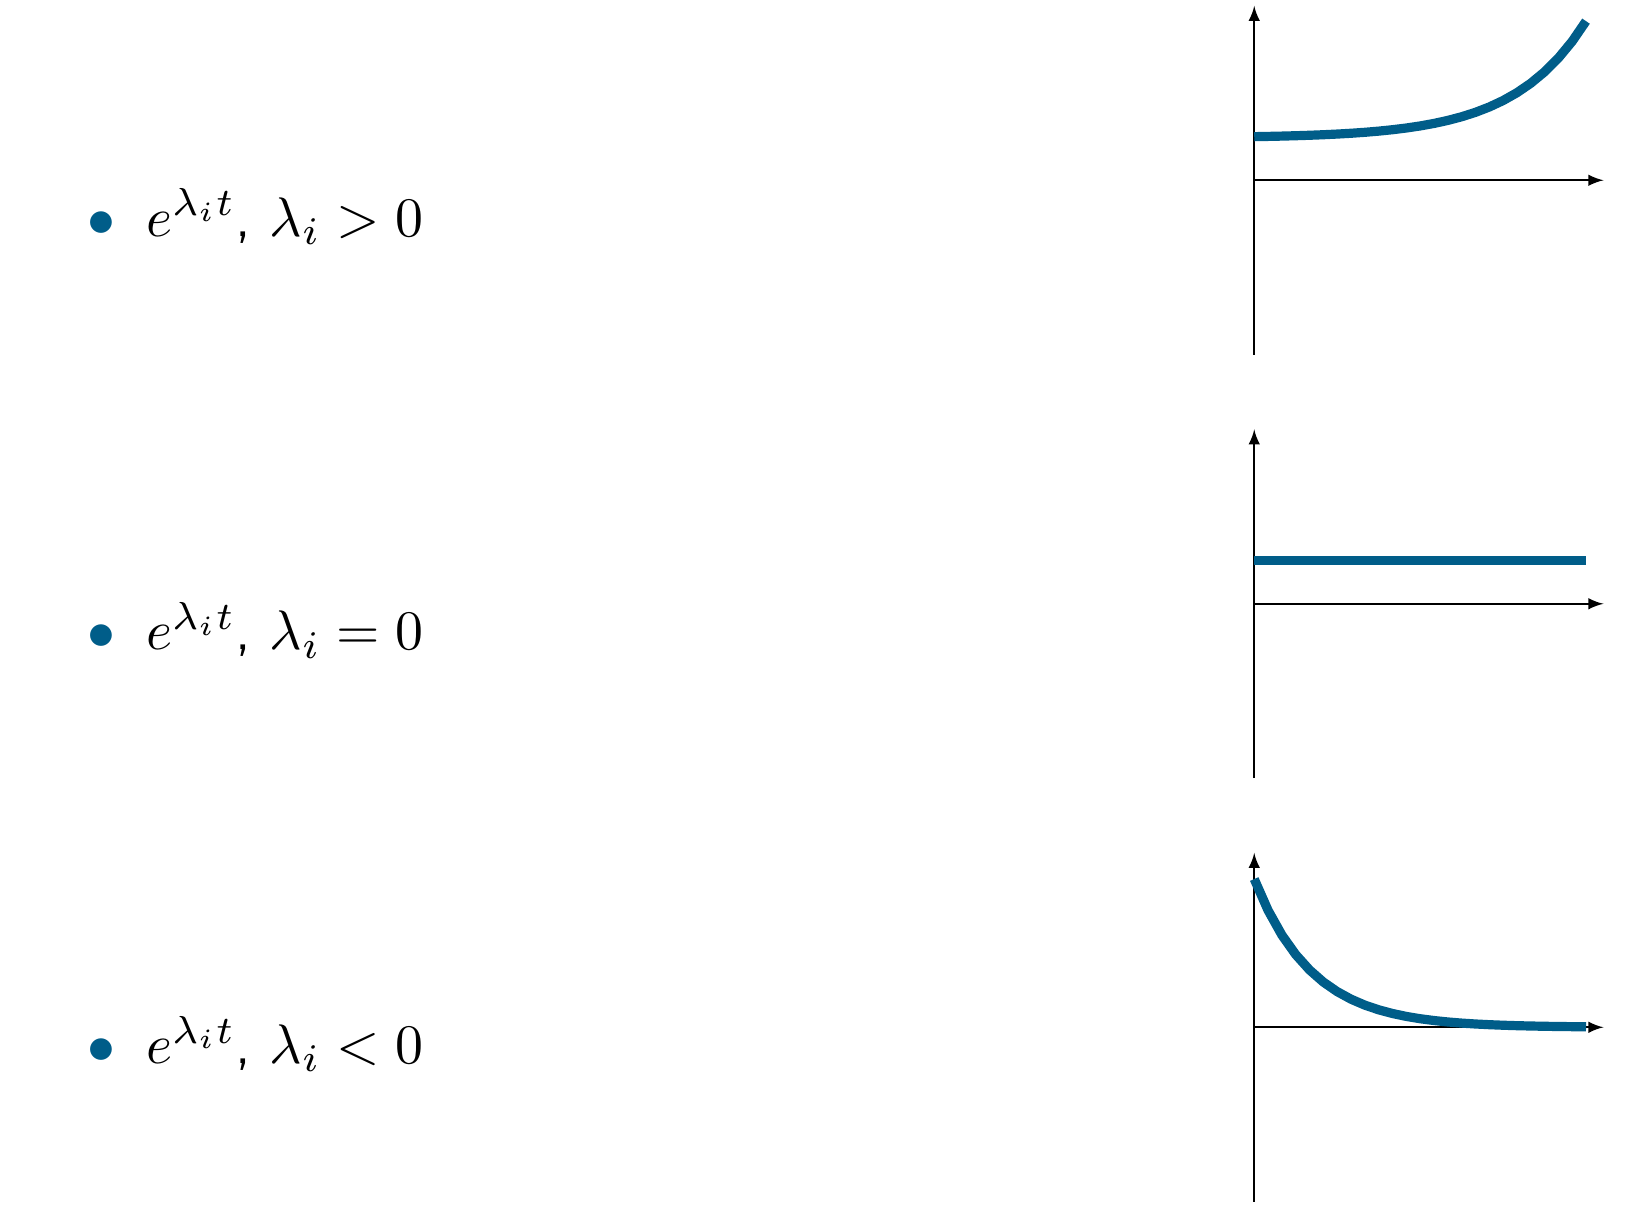
\includegraphics[scale=0.23]{Images/Autovalori_semplici.png}
\end{center}


\subsubsection*{Modi naturali: autovalori complessi coniugati semplici}
\begin{center}
    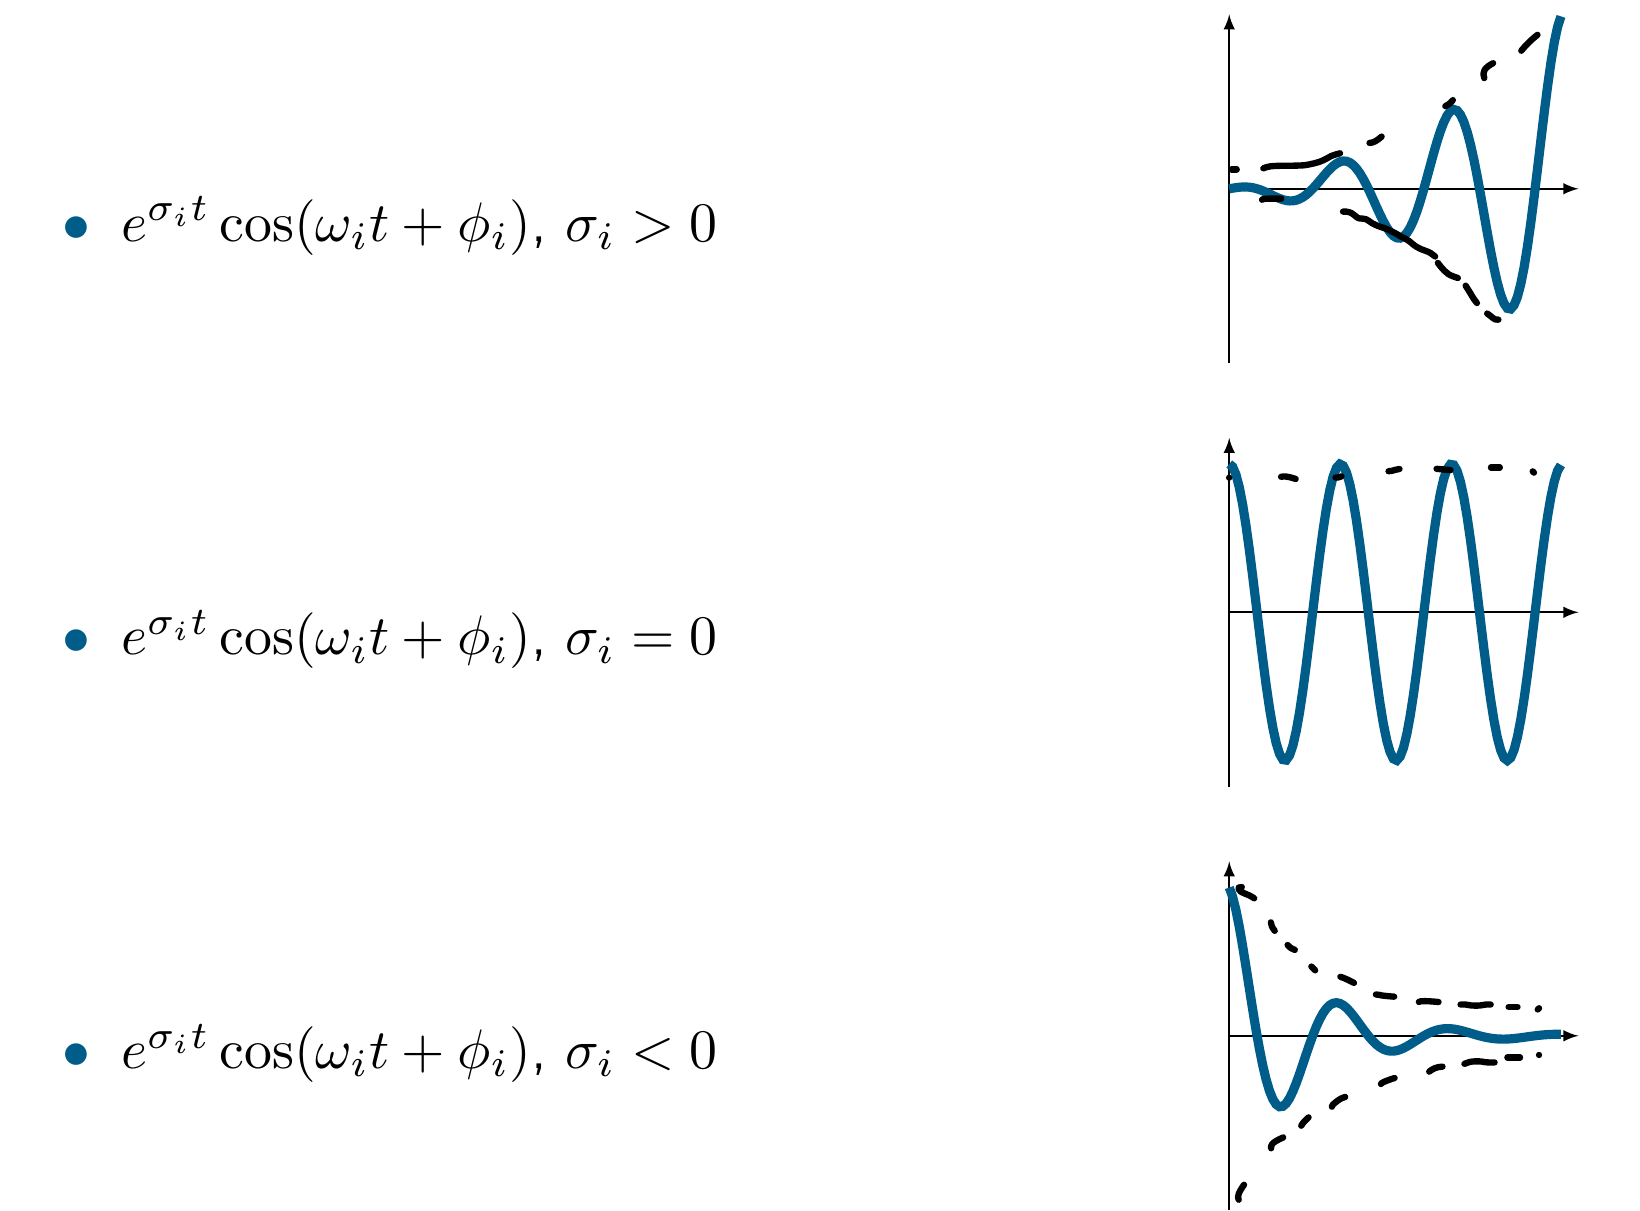
\includegraphics[scale=0.23]{Images/Autovalori_comlessi.png}
\end{center}

\begin{center}
    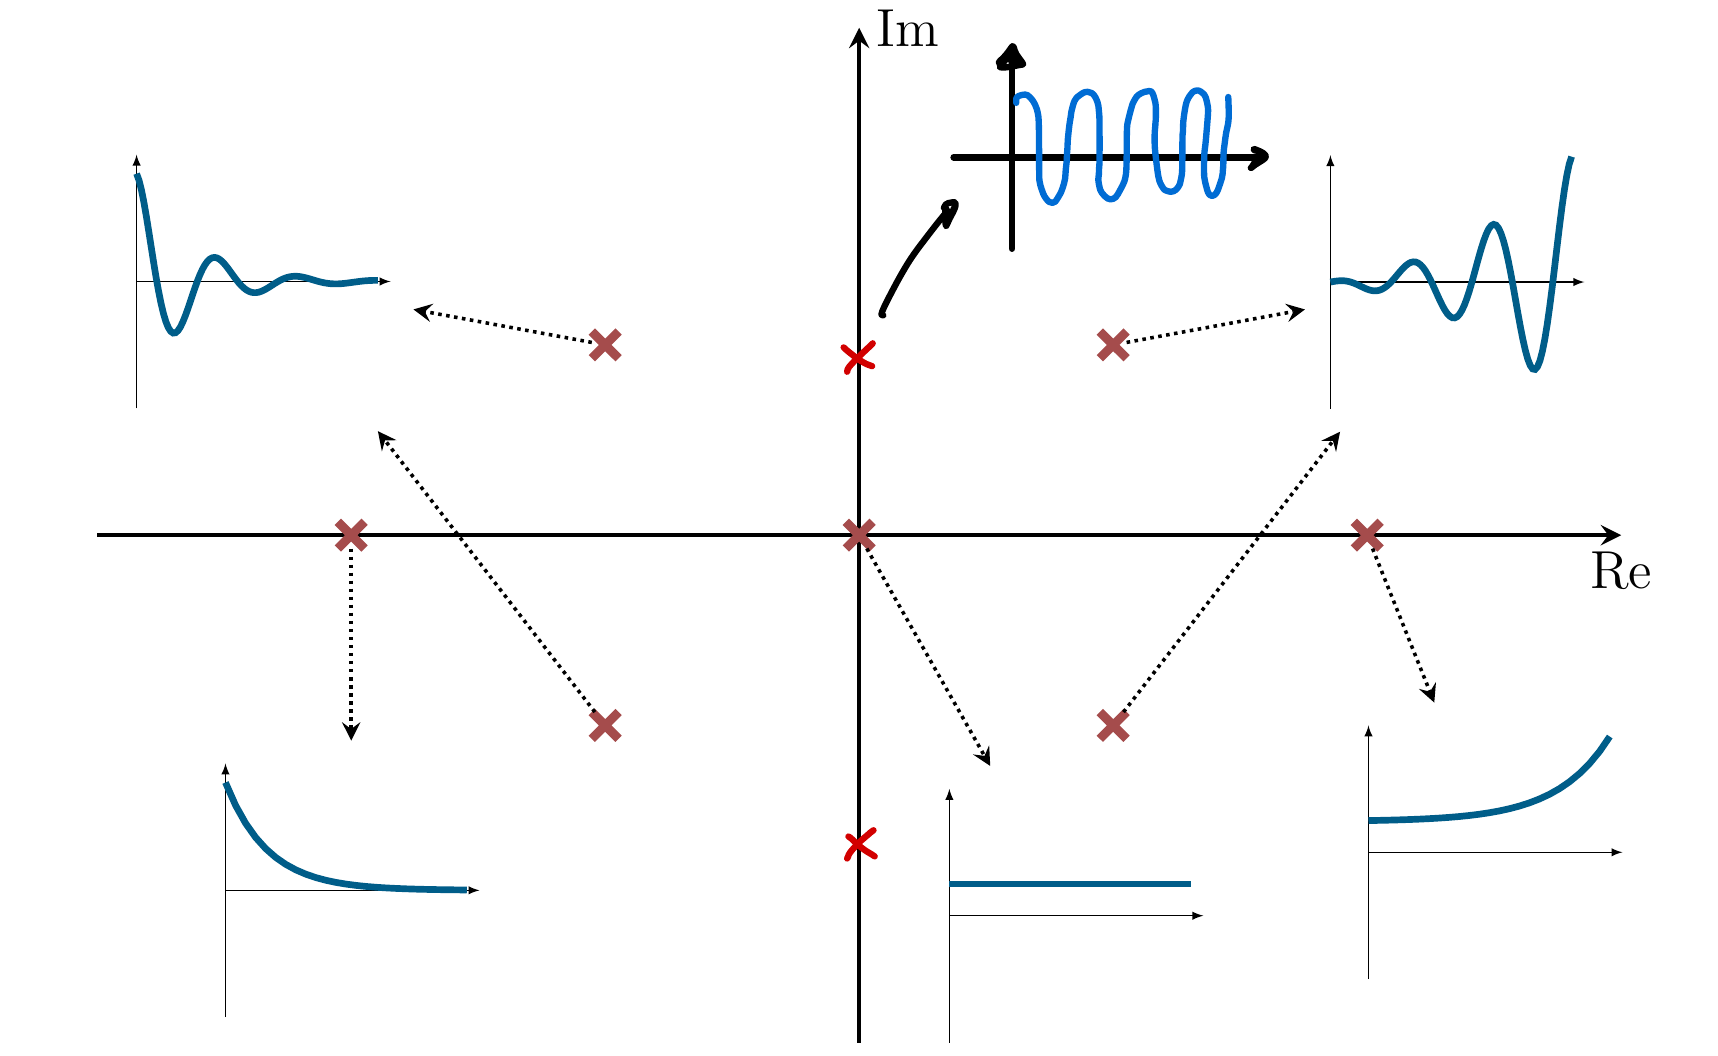
\includegraphics[scale=0.23]{Images/Esempio_autovalori.png}
\end{center}

\subsubsection{Esempio sui modi naturali}
\begin{equation}
    \begin{bmatrix}
        \dot x_1\\
        \dot x_2
    \end{bmatrix}
    =
    \begin{bmatrix}
        0 & 1\\
        a^2 & 0
    \end{bmatrix}
    \begin{bmatrix}
        x_1\\
        x_2
    \end{bmatrix}
\end{equation}

\begin{align*}
    p(\lambda) &= \det (\lambda I -A)\\
    &= \lambda^2 - a^2\\
    &\Rightarrow \begin{cases}
        \lambda_1 = a\\
        \lambda_2 = -a
    \end{cases}
\end{align*}
I modi naturali di questo sistema sono 
\begin{align*}
    &e^{at} & &e^{-at}
\end{align*}
Il modo $e^{at}$ diverge a infinito, il che non è una cosa "buona" per dei sistemi di controllo, perché ad esempio se si sta realizzando un sistema di controllo della velocità vuol dire che la mia velocità sta aumentando, mentre dovrebbe rimanere fissa in un range.\\
Non bisogna quindi focalizzarsi sul calcolare con precisione il valore dei modi naturali ma è importante conoscere come si comporta la loro parte reale.


\subsubsection{Esempio 1}
Consideriamo il seguente sistema LTI con $x \in \mathbb{R}^3 e u \in \mathbb{R}^3$
\begin{equation}
    \dot x(t) = \underbrace{\begin{bmatrix}
        0 & 1 & -1\\
        1 & -1 & -1\\
        2 & 1 & 3 
    \end{bmatrix}}_{A} x(t) +
    \underbrace{\begin{bmatrix}
        1 & 1 & 0\\
        0 & 1 & 1\\
        1 & 1 & 1
    \end{bmatrix}}_{B} u(t)
\end{equation}
Mediante un cambio di coordinate usando la matrice $T = \begin{bmatrix}
    0 & -1 & 1\\ 1 & 1 & -1\\ -1 & 0 & 1
\end{bmatrix}$ e ponendo $\hat x(t) = T x(T)$, il sistema si può riformulare come 
\begin{equation}
    \hat{\dot x} (t)= \underbrace{\begin{bmatrix}
        -1 & 1 & 0\\
        0 & -1 & 0\\
        0 & 0 & -2 
    \end{bmatrix}}_{\hat A = TAT^{-1}} \hat x(t) +
    \underbrace{\begin{bmatrix}
        1 & 0 & 0\\
        0 & 1 & 0\\
        0 & 0 & 1
    \end{bmatrix}}_{\hat B = TB} u(t)
\end{equation}
Gli autovalori di $\hat A$ sono $-1, -2$ con molteplicità algebrica $2,1$.
\vspace*{0.2cm}\\
Per calcolare l'evoluzione libera consideriamo la formula vista in precedenza
\begin{equation}
    \hat x_\ell  =e^{\hat A t}\hat x_0
\end{equation}
Calcoliamo quindi l'esponenziale di matrice $e^{\hat A t}$ per $\hat A = \begin{bmatrix}
    -1 & 1 & 0\\
    0 & -1 & 0\\
    0 & 0 & -2
\end{bmatrix}$
\begin{align*}
    e^{\hat A t} &= \sum_{k=0}^\infty \begin{bmatrix}
        -1 & 1 & 0\\
        0 & -1 & 0\\
        0 & 0 & -2
    \end{bmatrix}^k \frac{t^k}{k!}\\
    &= \begin{bmatrix}
        \sum\limits_{k=0}^\infty \frac{(-1)^k t^k}{k!} & t \sum\limits_{k=0}^\infty \frac{(-1)^k t^k}{k!} & 0\\
        0 & \sum\limits_{k=0}^\infty \frac{(-1)^k t^k}{k!} & 0\\
        0 & 0 & \sum\limits_{k=0}^\infty \frac{(-2)^k t^k}{k!}
    \end{bmatrix}\\
    &= \begin{bmatrix}
        e^{-t} & te^{-t} & 0\\
        0 & e^{-t} & 0\\
        0 & 0 & e^{-2t}
    \end{bmatrix}
\end{align*}
quindi l'evoluzione libera dello stato è
\begin{equation}
    \hat x_\ell = 
    \begin{bmatrix}
        e^{-t} & te^{-t} & 0\\
        0 & e^{-t} & 0\\
        0 & 0 & e^{-2t}
    \end{bmatrix} \hat x_0
\end{equation}
\begin{itemize}
\item Se ad esempio la condizione iniziale è $\hat x_0 = \begin{bmatrix} 1\\0\\0 \end{bmatrix}$, allora
\begin{equation}
    \hat x_\ell = \begin{bmatrix} e^{-t}\\0\\0 \end{bmatrix}
\end{equation}
Scriviamolo nello coordinate originali
\begin{equation}
    x_\ell(t) = \underbrace{\begin{bmatrix}
        1&1&0\\
        0&1&1\\
        1&1&1
    \end{bmatrix}}_{T^{-1}} \hat x_\ell (t) = 
    \begin{bmatrix}
        e^{-t}\\
        0\\
        e^{-t}
    \end{bmatrix}
\end{equation}
\item Se prendiamo come condizione iniziale $\hat x_0 = \begin{bmatrix} 0\\1\\0 \end{bmatrix}$, allora
\begin{equation}
    \hat x_\ell = \begin{bmatrix} te^{-t}\\e^{-t}\\0 \end{bmatrix}
\end{equation}
Scriviamolo nello coordinate originali
\begin{equation}
    x_\ell(t) = \underbrace{\begin{bmatrix}
        1&1&0\\
        0&1&1\\
        1&1&1
    \end{bmatrix} }_{T^{-1}} \hat x_\ell (t) = 
    \begin{bmatrix}
        e^{-t} + te^{-t}\\
        e^{-t}\\
        e^{-t} + te^{-t}
    \end{bmatrix}
\end{equation}


\item Se prendiamo come condizione iniziale $\hat x_0 = \begin{bmatrix} 0\\0\\1 \end{bmatrix}$. allora
\begin{equation}
    \hat x_\ell = \begin{bmatrix} 0\\0\\e^{-2t} \end{bmatrix}
\end{equation}
Nelle coordinate originali:
\begin{equation}
    x_\ell(t) = \underbrace{\begin{bmatrix}
        1&1&0\\
        0&1&1\\
        1&1&1
    \end{bmatrix} }_{T^{-1}} \hat x_\ell (t) = 
    \begin{bmatrix}
        0\\
        e^{-2t}\\
        e^{-2t}
    \end{bmatrix}
\end{equation}

\end{itemize}


\subsubsection{Esempio carrello}
\begin{align*}
    \dot x_1(t) &= x_2(t) \\
    \dot x_2(t) &= - \frac{k(t)}{M}x_1(t) + \frac{1}{M} u(t) \\
    y(t) &= x_1(t)
\end{align*}
\begin{align*}
    \begin{bmatrix}
        \dot x_1(t)\\
        \dot x_2(t)
    \end{bmatrix} &=
    \begin{bmatrix}
        0 & 1\\
        - \frac{k}{M} & 0
    \end{bmatrix}
    \begin{bmatrix}
        x_1(t)\\
        x_2(t)
    \end{bmatrix}
    +
    \begin{bmatrix}
        0\\
        \frac{1}{M}
    \end{bmatrix} u(t)
    \\
    y(t) &= \begin{bmatrix}
        1 & 0
    \end{bmatrix}
    \begin{bmatrix}
        x_1(t)\\
        x_2(t)
    \end{bmatrix} + 0 u(t)
\end{align*}
Consideriamo $k$ costante, quindi sistema LTI.\\
Gli autovalori della matrice $A$ sono $\lambda_1 = j \sqrt{\dfrac{k}{M}}, \lambda_2 = -j \sqrt{\dfrac{k}{M}}$ immaginari puri.
\vspace*{0.2cm}\\
Applichiamo un controllo $u = - hx_2$. Le equazioni di stato del sistema diventano:
\begin{align*}
    \dot x_1(t) &= x_2(t)\\
    \dot x_2(t) &= -\frac{k}{M}x_1(t) - \frac{h}{M}x_2(t)    
\end{align*}
in forma matriciale
\begin{align*}
    \begin{bmatrix}
        \dot x_1(t)\\
        \dot x_2(t)
    \end{bmatrix} &=
    \begin{bmatrix}
        0 & 1\\
        - \frac{k}{M} & -\frac{h}{M}x_2
    \end{bmatrix}
    \begin{bmatrix}
        x_1(t)\\
        x_2(t)
    \end{bmatrix}
\end{align*}
Quindi calcoliamo gli autovalori della matrice
\begin{align*}
    A &= 
    \begin{bmatrix}
        0 & 1\\
        - \frac{k}{M} & -\frac{h}{M}
    \end{bmatrix}
    &
    A - \lambda I &= 
    \begin{bmatrix}
        -\lambda & 1\\
        - \frac{k}{M} & -\frac{h}{M} - \lambda
    \end{bmatrix}
\end{align*}
calcolando il determinante e ponendolo a zero si trova il polinomio caratteristico associato a essa
\begin{align*}
    & & \lambda_1 &= - \frac{h}{2M} + \sqrt{\frac{h^2}{4M^2} - \frac{k}{M}}\\
    p(\lambda) &= \lambda^2 + \lambda \frac{h}{M} + \frac{k}{M} \Longrightarrow\\
    & & \lambda_2 &= - \frac{h}{2M} - \sqrt{\frac{h^2}{4M^2} - \frac{k}{M}}
\end{align*}
le cui soluzioni sono gli autovalori della matrice A.\\
Prendiamo ora in considerazione la quantità sotto radice; è evidente che se $h^2 > 4Mk$ gli autovalori sono reali, mentre se $h^2 < 4Mk$ sono complessi coniugati.
\vspace*{0.2cm}\\
Se invece $h^2 = 4Mk$, $\lambda_1 = \lambda_2 = -\frac{h}{2M}$, con molteplicità algebrica pari a 2. Si può dimostrare che la molteplicità geometrica è pari a 1, quindi il blocco di Jordan sarà $2 \times 2$ (guardare \ref{proprietà della matrice esponenziale})
\begin{align*}
    J &= TAT^{-1} = 
    \begin{bmatrix}
        - \frac{h}{2M} & 1\\
        0 & - \frac{h}{2M}
    \end{bmatrix}
    &
    e^{Jt} &= e^{- \frac{h}{2M}t}
    \begin{bmatrix}
        1 & t\\
        0 & 1
    \end{bmatrix}
\end{align*}
\begin{equation}
    \hat x_\ell = 
    \begin{bmatrix}
        e^{- \frac{h}{2M}t} \hat x_1(0) + t e^{- \frac{h}{2M}t} \hat x_2(0) \\
        e^{- \frac{h}{2M}t} \hat x_2(0)
    \end{bmatrix}
    =
    \begin{bmatrix}
        \hat x_{1 \ell}(t)\\
        \hat x_{2 \ell}(t)
    \end{bmatrix}
\end{equation}
Quindi i modi naturali del sistema sono
\begin{align*}
    &e^{- \frac{h}{2M}t} & &t e^{- \frac{h}{2M}t}  
\end{align*}
da notare che anche si effettua il cambio di coordinate i modi del sistema non cambiano.
\begin{itemize}
    \item Supponiamo $\hat x(0) = \begin{bmatrix} 1\\0 \end{bmatrix}$, allora
    \begin{equation}
        \hat x_\ell (t) = 
        \begin{bmatrix}
            e^{- \frac{h}{2M}t} \hat x_1(0)\\0
        \end{bmatrix}
    \end{equation}
    \item Supponiamo $\hat x(0) = \begin{bmatrix} 0\\1 \end{bmatrix}$, allora
    \begin{equation}
        \hat x_\ell (t) = 
        \begin{bmatrix}
            0\\e^{- \frac{h}{2M}t} \hat x_2(0)
        \end{bmatrix}
    \end{equation}
    \begin{center}
    \begin{tikzpicture}
            \begin{axis}[
                xmin=0,xmax=20,
                ymin=0,ymax=1,
                axis x line=middle,
                axis y line=middle,
                xlabel={$x$},
                ylabel={$y$},
                ]
                \addplot[domain=0:20, samples=100]{x * exp(-2/4 * x)}node   [pos=0.1,anchor=south west]{$y=t e^{-\frac{h}{2M}t}$};
            \end{axis}
        \end{tikzpicture}
    \end{center}
    Si nota dal grafico che se $- \dfrac{h}{2M}$ è "grande" il modo va a zero, quindi sono in un punto di equilibrio.
    \item Se $h = 4Mk = 0$ con $M >0,h=0,k=0$, il sistema diventa
    \begin{equation}
        \begin{bmatrix}
            \dot x_1(t)\\
            \dot x_2(t)
        \end{bmatrix} =
        \begin{bmatrix}
            0 & 1\\
            0 & 0
        \end{bmatrix}
        \begin{bmatrix}
            x_1(t)\\
            x_2(t)
        \end{bmatrix}
    \end{equation}
    i cui modi naturali sono $1,t$. È evidente come si possano scrivere queste equazioni differenziali come combinazione lineare dei modi:
    \begin{align*}
        x_1(t) &= x_1(0) + x_2(0)t\\
        x_2(t) &= x_2(0) 
    \end{align*}
\end{itemize}

\subsection{Stabilità interna}
\subsubsection{Richiami sull'equilibrio di un sistema}
Prendiamo un sistema lineare tempo invariante 
\begin{equation}
    \dot x(t) = f(x(t), u(t))
\end{equation}
Poniamo $u(t) = u_e \ \forall t \geq 0$, allora
\begin{equation}
    \dot x(t) = f(x(t), u_e) \tag*{$x(0)=x_0$}
\end{equation}
Esiste, per un sistema di questo tipo, una $x_e$ tale che se $x(0)=x_e \Longrightarrow x(t) = x_e \ \forall t \geq 0$, quindi tale che se lo stato iniziale è costante la $x(t)$ rimane costante in ogni istante di tempo?
\vspace*{0,2cm}\\
Chiamo $x_e$ equilibrio, $(x_e,u_e)$ la chiamo coppia stato-ingresso di equilibrio.
\vspace*{0.2cm}\\
Proprietà fondamentale di una coppia di equilibrio è che
\begin{equation}
    f(x_e,u_e) = 0
\end{equation}


\subsubsection{Definizioni}
Per sistemi tempo-invarianti (anche se si può generalizzare) la \textit{stabilità interna} di un sistema è l'insieme delle conseguenze sulla traiettoria legate a incertezze sullo stato iniziale con ingressi fissi e noti.


\subsubsection{Stabilità interna per sistemi non forzati}
\begin{equation}
    \dot x(t) = f(x(t)) \tag*{$x_e$ equilibrio}  
\end{equation}
\textbf{Equilibrio stabile:} uno stato di equilibrio $x_e$ si dice stabile se $\forall \epsilon >0, \exists \delta >0$ tale che $\forall x_0 : || x_0-x_e || \leq \delta$ allora risulti $ || x(t) - x_e || < \epsilon \ \forall t \geq 0$. 
\vspace*{0.2cm}\\
\textbf{Equilibrio instabile:} uno stato di equilibrio $x_e$ si dice instabile se non è stabile.
\vspace*{0.2cm}\\
\textbf{Equilibrio attrattivo:} uno stato di equilibrio $x_e$ si dice  attrattivo se $\exists \delta$ tale che $\forall x_0: || x_0-x_e || \leq \delta$ allora risulti $\lim\limits_{t \rightarrow \infty} || x(t)-x_e ||=0$; quindi se il sistema è in equilibrio solo a infinito.
\vspace*{0.2cm}\\
\textbf{Equilibrio asintoticamente stabile:} uno stato di equilibrio $x_e$ si dice asintoticamente stabile se è stabile e attrattivo.
\vspace*{0.2cm}\\
\textbf{Equilibrio marginalmente stabile:} uno stato di equilibrio si dice marginalmente stabile se è stabile ma non asintoticamente.

\subsubsection*{Rappresentazione grafica di un sistema in equilibrio stabile}
\begin{center}
    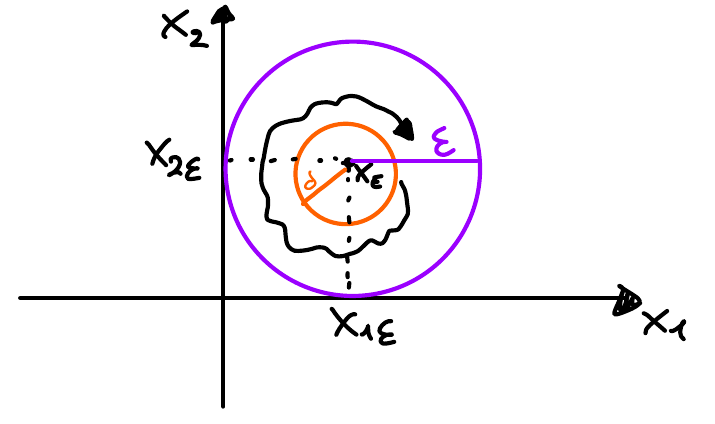
\includegraphics[scale=0.3]{Images/Equilibrio_stabile.png}
\end{center}

\subsubsection*{Rappresentazione grafica di un sistema in equilibrio attrattivo}
\begin{center}
    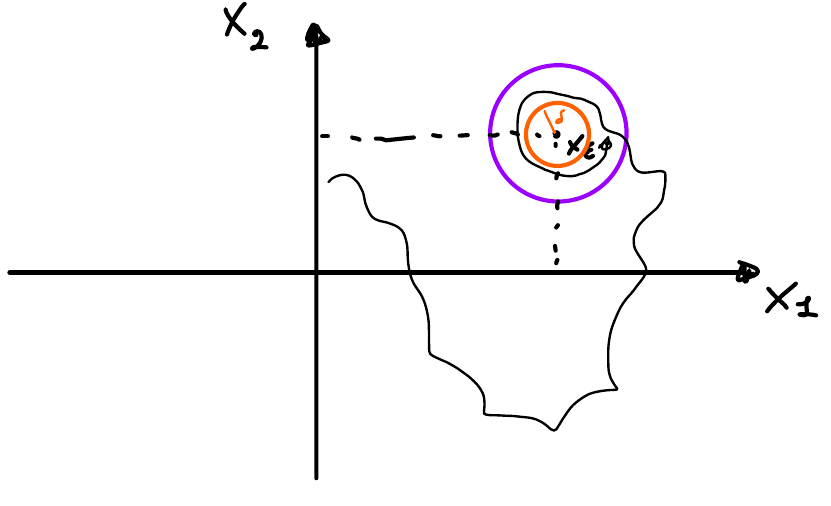
\includegraphics[scale=0.3]{Images/Equilibrio_attrattivo.png}
\end{center}

\subsubsection{Osservazioni}
Le definizioni date sottintendono la parola locale, ovvero che la proprietà vale in un intorno dello stato di equilibrio $x_e$.
\vspace*{0.2cm}\\
\textbf{Stabilità globale:} le proprietà di stabilità e asintotica stabilità sono globali se valgono per ogni $x \in \mathbb{R}^n$, invece che valere solo per $x_0$ tale che $|| x(0)-x_e || \leq \delta $.
\vspace*{0.2cm}\\
\textbf{Stabilità di una traiettoria:} le definizioni di stabilità si possono generalizzare a una traiettoria $\overline{x}(t), t \geq 0$.
\begin{center}
    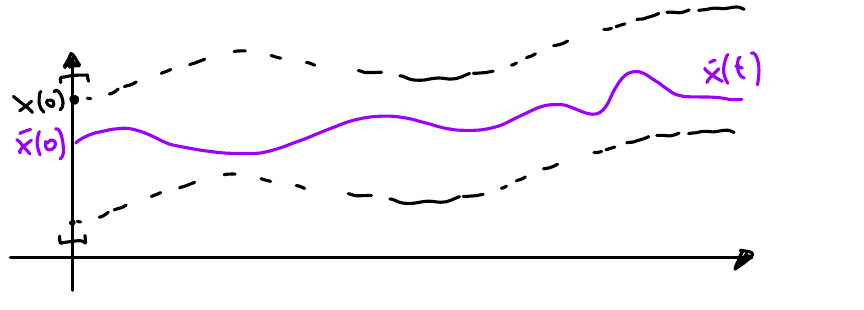
\includegraphics[scale=0.3]{Images/Stabilita_traiettoria.png}
\end{center}

\subsection{Stabilità interna di sistemi LTI}
Nei sistemi lineari $x=0$ è sempre un equilibrio.\\
Per sistemi lineari si può dimostrare che tutti gli equilibri e tutte le traiettorie hanno le stesse proprietà di stabilità, tutte uguali a $x=0$. Per questo motivo si parla di \textbf{stabilità del sistema}.
\subsubsection*{Dimostrazione}
\begin{equation}
    \begin{rcases}
        \dot x(t) = Ax(t) + Bu(t)\\
        u(t) = u_e \ \ \forall t \geq 0
    \end{rcases}
    \Longrightarrow Ax_e + Bu_e = 0
\end{equation}
Sia $\tilde{x}(t) := x(t) - x_e$, allora
\begin{align*}
    \dot{\tilde{x}}(t) &= \dot x(t) - \underbrace{\frac{d}{dt}x_e}_{0}\\
    &=Ax(t)+Bu_e\\
    &=A(\tilde{x}(t)+x_e)+Bu_e\\
    &=A \tilde{x}(t) + \underbrace{Ax_e+Bu_e}_{0}
\end{align*}
quindi
\begin{equation}
    \dot{\tilde{x}}(t) = A \tilde{x}(t)
\end{equation}
Concludiamo che
\begin{equation}
    \tilde{x}=0 \Longleftrightarrow x = x_e
\end{equation}
cioè per studiare l'equilibrio di un sistema nel generico punto $x_e$ posso studiare l'equilibrio del sistema nell'origine.




\subsubsection*{Teorema} \label{Teorema parte reale negativa}
Un sistema LTI è \textbf{asintoticamente stabile} \underline{se e solo se} tutti gli autovalori hanno parte reale strettamente negativa.
\vspace*{0.1cm}\\
\textbf{N.B.} Se gli autovalori hanno parte reale strettamente negativa i modi del sistema tendono a 0 (\ref{Modi naturali: autovalori reali semplici}).

\subsubsection*{Teorema}
Un sistema LTI è stabile se e solo se tutti gli autovalori hanno parte reale minore o uguale a zero e tutti gli autovalori a parte reale nulla hanno molteplicità geometrica uguale alla molteplicità algebrica (i mini blocchi di Jordan associati hanno dimensione uno).

\subsubsection*{Osservazione}
Si ha instabilità se almeno un autovalore ha parte reale positiva o se almeno un autovalore con parte reale nulla ha molteplicità algebrica maggiore della molteplicità geometrica.


\subsubsection*{Osservazione}
La stabilità asintotica di sistemi LTI è sempre globale
\begin{align*}
    x(0) &= x_0 \Longrightarrow x(t) \ \ t \geq 0 \\
    x(0) &= \alpha x_0 \Longrightarrow \alpha x(t) \ \ t \geq 0
\end{align*}


\subsubsection*{Proprietà}
Se un sistema LTI è globalmente asintoticamente stabile, $x=0$ è l'unico equilibrio.\\
\textbf{Nota:} anche per sistemi \underline{non lineari} se $x_e$ è GAS (Globalmente Asintoticamente Stabile) allora è l'unico equilibrio.
\vspace*{0.1cm}\\
Questo perché



\subsubsection{Esempio stabilità del sistema carrello}
\begin{align*}
    \dot x_1(t) &= x_2(t) \\
    \dot x_2(t) &= - \frac{k(t)}{M}x_1(t) + \frac{1}{M} u(t) \\
    y(t) &= x_1(t)
\end{align*}
\begin{align*}
    \begin{bmatrix}
        \dot x_1(t)\\
        \dot x_2(t)
    \end{bmatrix} &=
    \begin{bmatrix}
        0 & 1\\
        - \frac{k}{M} & 0
    \end{bmatrix}
    \begin{bmatrix}
        x_1(t)\\
        x_2(t)
    \end{bmatrix}
    +
    \begin{bmatrix}
        0\\
        \frac{1}{M}
    \end{bmatrix} u(t)
    \\
    y(t) &= \begin{bmatrix}
        1 & 0
    \end{bmatrix}
    \begin{bmatrix}
        x_1(t)\\
        x_2(t)
    \end{bmatrix} + 0 u(t)
\end{align*}
Consideriamo $k$ costante, quindi sistema LTI.\\
Gli autovalori della matrice $A$ sono $\lambda_1 = j \sqrt{\dfrac{k}{M}}, \lambda_2 = -j \sqrt{\dfrac{k}{M}}$ immaginari puri, quindi sistema semplicemente (marginalmente) stabile.
\vspace*{0.2cm}\\
Se applichiamo $u=-h x_2$ gli autovalori diventano $\lambda_1 = - \frac{h}{2M} + \sqrt{\dfrac{h^2}{4M^2}-\dfrac{k}{M}}$ e $\lambda_2 = \dfrac{h}{2M} - \sqrt{\dfrac{h^2}{4M^2}-\dfrac{k}{M}}$.\\
\begin{itemize}
    \item Se $h^2 \geq 4Mk$ gli autovalori sono 2 reali negativi, quindi il sistema è asintoticamente stabile;
    \item Se $h^2 < 4Mk$ gli autovalori sono 2 complessi coniugati con parte reale negativa, quindi il sistema è asintoticamente stabile;
    \item Se $h^2 = 4Mk$, $\lambda_1 = \lambda_2 = -\frac{h}{2M}$, con molteplicità algebrica pari a 2. Si può dimostrare che la molteplicità geometrica è pari a 1, quindi il blocco di Jordan sarà $2 \times 2$ (guardare \ref{proprietà della matrice esponenziale})
    \begin{align*}
        J &= TAT^{-1} = 
        \begin{bmatrix}
            - \frac{h}{2M} & 1\\
            0 & - \frac{h}{2M}
        \end{bmatrix}
        &
        e^{Jt} &= e^{- \frac{h}{2M}t}
        \begin{bmatrix}
            1 & t\\
            0 & 1
        \end{bmatrix}
    \end{align*}
    Gli autovalori sono a parte reale negativa, quindi il sistema è asintoticamente stabile;
    \item Se $h=k=0 \Longrightarrow \lambda_1=\lambda_2=0$, quindi il sistema è instabile.
\end{itemize}





\subsection{Retroazione dello stato}
Prendiamo un sistema lineare tempo invariante
\begin{align*}
    \dot x(t) &= Ax(t) + Bu(t)\\
    y(t) &= Cx(t) + Du(t) 
\end{align*}
Supponendo di misurare l'intero stato, ovvero se $x(t)=y(t)$, allora possiamo progettare
\begin{equation}
    u(t) = Kx(t) + v(t)
\end{equation}
con $K \in \mathbb{R}^{m \times n}$ una matrice di guadagni e $v(t)$ un ulteriore ingresso per il sistema retroazionato
\begin{equation}
    \dot x(t) = (A+BK)x(t)+Bv(t)
\end{equation}
Se vogliamo il sistema in anello chiuso asintoticamente stabile allora dobbiamo progettare $K$ tale che $(A + BK)$ abbia autovalori tutti a parte reale negativa.\\
\textbf{Nota:} la possibilità di scegliere gli autovalori di $(A + BK)$ (e.g., per renderli tutti a parte reale negativa) dipende dalla coppia $(A, B)$ ed è legata alla proprietà di \textbf{raggiungibilità}.
\vspace*{0.1cm}\\
Se non è possibile misurare l'intero stato, ovvero se $y(t) \neq x(t)$, esistono tecniche per ricostruire lo stato a partire dalle misure mediante sistemi ausiliari chiamati \textbf{osservatori}.\\
Se sia possibile o meno ricostruire lo stato dipende dalla coppia $(A, C)$ ed è legato alla proprietà di \textbf{osservabilità}.




\subsection{Linearizzazione di sistemi in non lineari (tempo invarianti)}
Prendiamo un  sistema non lineare tempo invariante
\begin{align*}
    \dot x(t) &= f (x(t), u(t))\\
    y(t) &= h(x(t), u(t))
\end{align*}
Sia $(x_e,u_e)$ una coppia di equilibrio, $f(x_e,u_e)=0$, consideriamo una traiettoria a partire da uno stato stato iniziale $x(0)=x_e+ \tilde{x}_0$ 
\begin{align*}
    x(t) &= x_e + \tilde{x}(t)\\
    u(t) &= u_e + \tilde{u}(t)
\end{align*}
con $y(t) = h(x_e , u_e ) + \tilde{y}(t) = y_e + \tilde{y}(t)$.\\
Essendo una traiettoria vale
\begin{align*}
    \frac{d}{dt}(x_e + \tilde{x}(t)) &= f (x_e + \tilde{x}(t), u_e + \tilde{u}(t))\\
    y_e + \tilde{y}(t) &= h(x_e+\tilde{x}(t), u_e+ \tilde{u}(t))
\end{align*}
Sviluppando in serie di Taylor (con $f$ e $h$ sufficientemente regolari) in $(xe , ue )$ \footnote[1]{i termini del tipo $\frac{\partial}{\partial x}f(x,u)$ vengono chiamati \textit{Jacobiani}}
\begin{align*}
    \frac{d}{dt}(x_e + \tilde{x}(t)) &= \underbrace{f(x_e,u_e)}_{0} + \underbrace{\frac{\partial}{\partial x}f(x,u)\bigg|_{\substack{\text{$x=x_e$} \\ \text{$u=u_e$}}}}_{A_e} \tilde{x}(t) + \underbrace{\frac{\partial}{\partial u}f(x,u)\bigg|_{\substack{\text{$x=x_e$} \\ \text{$u=u_e$}}}}_{B_e} \tilde{u(t)} + \T{term. ord. sup.}\\
    y_e+\tilde{y}(t) &= h(x_e,u_e) + \underbrace{\frac{\partial}{\partial x}h(x,u) \bigg|_{\substack{\text{$x=x_e$} \\ \text{$u=u_e$}}}}_{C_e} \tilde{x}(t) + \underbrace{\frac{\partial}{\partial u}h(x,u) \bigg|_{\substack{\text{$x=x_e$} \\ \text{$u=u_e$}}}}_{D_e} \tilde{u}(t) + \T{term. ord. sup.}
\end{align*} 
\begin{align*}
    A &= \frac{\partial f(x,u)}{\partial x} \Biggl |_{\substack{\text{$x=x_e$} \\ \text{$u=u_e$}}} &
    B &= \frac{\partial f(x,u)}{\partial u} \Biggl |_{\substack{\text{$x=x_e$} \\ \text{$u=u_e$}}}\\
    C &= \frac{\partial g(x,u)}{\partial x} \Biggl |_{\substack{\text{$x=x_e$} \\ \text{$u=u_e$}}} &
    D &= \frac{\partial g(x,u)}{\partial u} \Biggl |_{\substack{\text{$x=x_e$} \\ \text{$u=u_e$}}}\\
\end{align*}
quindi
\begin{align*}
    \tilde{\dot x}(t) &= A_e \tilde{x}(t) + B_e \tilde{u}(t) + \T{term. ord. sup.} \tag*{$\tilde{x}(0) = \tilde{x}_0$}\\
    \tilde{y}(t) &= C_e \tilde{x}(t) + D_e\tilde{u}(t) + \T{term. ord. sup.}
\end{align*}
Se consideriamo i termini di ordine superiore come un resto $\mathcal{R}(x,u)$ si osserva che
\begin{equation}
    \lim_{||(x,u)||\rightarrow 0} \frac{||\mathcal{R}(\tilde{x},\tilde{u})||}{||(\tilde{x},\tilde{u})||} = 0
\end{equation}
di fatto è come se si avesse $\lim\limits_{x \rightarrow 0}\dfrac{x^2}{x}$.\\
Quindi le due equazioni di prima si possono approssimare
\begin{align*}
    \tilde{\dot x}(t) &\approx A_e \tilde{x}(t) + B_e \tilde{u}(t)\\
    \tilde{y}(t) &\approx C_e \tilde{x}(t) + D_e\tilde{u}(t) 
\end{align*}
Il sistema linearizzato è
\begin{align*}
    \Delta \dot x(t) &= A_e \Delta x(t) + B_e \Delta u(t)\\
    \Delta y(t) &= C_e \Delta x(t) + D_e \Delta u(t)
\end{align*}
\textbf{N.B.} il pedice 'e' è una puntualizzazione ulteriore per sottolineare il fatto che le matrici sono valutate all'equilibrio, in altri testi potrebbero non avere questo pedice.
\vspace*{0.2cm}\\
Le traiettorie del sistema non lineare soddisfano
\begin{align*}
    x(t) &= x_e + \tilde{x}(t) \approx x_e + \Delta x(t)\\
    u(t) &= u_e + \tilde{u}(t) \approx u_e + \Delta u(t)\\
    y(t) &= y_e + \Delta y(t) \approx y_e + \Delta y(t) 
\end{align*}
per variazioni sufficientemente piccole.
\vspace*{0.1cm}\\
\textbf{Nota:} $(\Delta x(t),\Delta u(t)), t \geq 0$ traiettoria del sistema linearizzato.



\subsubsection{Esempio pendolo}
\begin{align*}
    \dot x_1(t) &= x_2(t) = f_1(x(t),u(t))\\
    \dot x_2(t) &= - \frac{g}{l} \sin(x_1(t)) - \frac{b}{M \ell^2}x_2(t) + \frac{1}{M \ell^2} u(t) = f_2(x(t),u(t))
\end{align*}
$(x_e,u_e)$ coppia di equilibrio
\begin{equation}
    f(x_e,u_e)=0 \Rightarrow 
    \begin{cases}
        x_{2e}=0\\
        - \dfrac{g}{\ell} \sin(x_{1e}) - \dfrac{b}{M \ell^2}x_{2e} + \dfrac{1}{M \ell^2}u_e
    \end{cases}
\end{equation}
Prendiamo come equilibrio $x_e = \begin{bmatrix} x_{1e}\\0 \end{bmatrix}$, allora
\begin{align*}
    &- \dfrac{g}{\ell} \sin(x_{1e}) - \dfrac{b}{M \ell^2} \cdot 0 + \dfrac{1}{M \ell^2}u_e = 0\\
    \Longrightarrow & u_e = gM\ell \sin(X_{1e})
\end{align*}
Eseguiamo la linearizzazione intorno a $(x_e,u_e)$
\begin{equation}
    \Delta \dot x(t) = A_e \Delta x(t) + B_e \Delta u(t)
\end{equation}
%calcolo matrice A_e
\begin{align*}
    \underbrace{A_e}_{\frac{\partial f(x,u)}{\partial x}\big|_{\substack{\text{$x=x_e$} \\ \text{$u=u_e$}}}} &=
    \begin{bmatrix}
        \dfrac{\partial f_1(x,u)}{\partial x_1} & \dfrac{\partial f_1(x,u)}{\partial x_2}\\
        \dfrac{\partial f_2(x,u)}{\partial x_1} & \dfrac{\partial f_2(x,u)}{\partial x_2}
    \end{bmatrix}_{\substack{\text{$x=x_e$} \\ \text{$u=u_e$}}}\\ &=
    \begin{bmatrix}
        0 & 1\\
        -\dfrac{g}{\ell}\cos(x_1) & -\dfrac{b}{M \ell^2}
    \end{bmatrix}_{\substack{\text{$x=x_e$} \\ \text{$u=u_e$}}} \\ &=
    \begin{bmatrix}
        0 & 1\\
        -\dfrac{g}{\ell}\cos(x_{1e}) & -\dfrac{b}{M \ell^2}
    \end{bmatrix}
\end{align*}
%calcolo matrice B_e
\begin{align*}
    \underbrace{B_e}_{\frac{\partial f(x,u)}{\partial u}\big|_{\substack{\text{$x=x_e$} \\ \text{$u=u_e$}}}} &=
    \begin{bmatrix}
        \dfrac{\partial f_1(x,u)}{\partial u}\\
        \dfrac{\partial f_2(x,u)}{\partial u} 
    \end{bmatrix}_{\substack{\text{$x=x_e$} \\ \text{$u=u_e$}}}\\ &=
    \begin{bmatrix}
        0\\
        \dfrac{1}{M \ell^2}
    \end{bmatrix}_{\substack{\text{$x=x_e$} \\ \text{$u=u_e$}}}\\ &=
    \begin{bmatrix}
        0\\
        \dfrac{1}{M \ell^2}
    \end{bmatrix}
\end{align*}
\begin{itemize}
    \item se $x_e = \begin{bmatrix} 0\\0 \end{bmatrix}$ e $u_e = 0$
    \begin{align*}
        A_e &= 
        \begin{bmatrix}
            0 & 1\\
            -\dfrac{g}{\ell} & -\dfrac{b}{M \ell^2}
        \end{bmatrix} 
        &
        B_e &=
        \begin{bmatrix}
            0\\
            \dfrac{1}{M \ell^2}
        \end{bmatrix}
    \end{align*}
    \item se $x_e=\begin{bmatrix} \pi\\0 \end{bmatrix}$ e $u_e=0$
    \begin{align*}
        A_e &= 
        \begin{bmatrix}
            0 & 1\\
            \dfrac{g}{\ell} & -\dfrac{b}{M \ell^2}
        \end{bmatrix} 
        &
        B_e &=
        \begin{bmatrix}
            0\\
            \dfrac{1}{M \ell^2}
        \end{bmatrix}
    \end{align*}
    \item se $x_e=\begin{bmatrix} \pi/2 \\0 \end{bmatrix}$ e $u_e=MG\ell$
    \begin{align*}
        A_e &= 
        \begin{bmatrix}
            0 & 1\\
            0 & -\dfrac{b}{M \ell^2}
        \end{bmatrix} 
        &
        B_e &=
        \begin{bmatrix}
            0\\
            \dfrac{1}{M \ell^2}
        \end{bmatrix}
    \end{align*}
\end{itemize}



\subsubsection{Stabilità di 3 sistemi lineari (linearizzzione intorno a 3 diversi equilibri)}
\begin{enumerate}
    \item 
    \begin{align*}
        A_e &= \begin{bmatrix} 0&1\\-\dfrac{g}{\ell}&-\dfrac{b}{M \ell^2} \end{bmatrix} & p(\lambda) &= \lambda \left( \lambda + \frac{b} +{M\ell^2} \right) + \frac{g}{\ell}\\
        & & &=\lambda^2 + \frac{b}{M\ell^2}\lambda + \frac{g}{\ell}
    \end{align*}
    \begin{equation}
        \lambda_{1/2} = - \frac{b}{2M \ell^2} \pm \sqrt{\left(\frac{b}{2M\ell^2}\right) - \frac{g}{\ell}}
    \end{equation}
    Abbiamo 2 autovalori a parte reale negativa, quindi il sistema linearizzato è \textit{asintoticamente stabile (globalmente)}.

    \item 
    \begin{align*}
        A_e &= \begin{bmatrix} 0&1\\\dfrac{g}{\ell}&-\dfrac{b}{M \ell^2} \end{bmatrix} & p(\lambda) &= \lambda \left( \lambda + \frac{b} {M\ell^2} \right) - \frac{g}{\ell}\\
        & & &=\lambda^2 + \frac{b}{M\ell^2}\lambda - \frac{g}{\ell}
    \end{align*}
    \begin{equation}
        \lambda_{1/2} = - \frac{b}{2M \ell^2} \pm \sqrt{\underbrace{\left(\frac{b}{2M\ell^2}\right) + \frac{g}{\ell}}_{>0}} \Longrightarrow
        \begin{cases}
            \lambda_{1} = - \dfrac{b}{2M \ell^2} - \sqrt{\left(\dfrac{b}{2M\ell^2}\right) + \dfrac{g}{\ell}} <0\\
            \\
            \lambda_{2} = - \dfrac{b}{2M \ell^2} + \sqrt{\left(\dfrac{b}{2M\ell^2}\right) + \dfrac{g}{\ell}} >0
        \end{cases}
    \end{equation}
    Dato che abbiamo un autovalore a parte reale positiva il sistema è \textit{instabile}.

    \item 
    Se poniamo $x_e = \begin{bmatrix} \pi/2\\ 0 \end{bmatrix}$ e $M_e = Mg\ell$
    \begin{align*}
        A_e &= \begin{bmatrix} 0&1\\ 0&-\dfrac{b}{M \ell^2} \end{bmatrix} & p(\lambda) &= \lambda \left( \lambda + \frac{b} {M\ell^2} \right)
    \end{align*}
    \begin{align*}
        \lambda_1 &= 0 & \lambda_2&=-\frac{b}{M\ell^2}
    \end{align*}
    Il sistema linearizzato è \textit{stabile}, ma non asintoticamente, cioè marginalmente stabile (ricordando \ref{Teorema parte reale negativa})
\end{enumerate}



\subsection{Stabilità e linearizzazione}
\subsubsection*{Teorema}
Dato un sistema non lineare tempo invariante, $\dot x(t)=f(x(t),u(t))$, sia $x_e,u_e$ una coppia di equilibrio. Se il sistema linearizzato intorno a $(x_e,u_e)$ è asintoticamente stabile, allora l'equilibrio $x_e$, relativo all'ingresso $u_e$, è (localmente) asintoticamente stabile.

\subsubsection*{Teorema}
Dato un sistema non lineare tempo invariante, $\dot x(t)=f(x(t),u(t))$, sia $x_e,u_e$ una coppia di equilibrio. Se il sistema linearizzato intorno a $(x_e,u_e)$ ha almeno un autovalore a parte reale positiva, allora l'equilibrio $x_e$, relativo all'ingresso $u_e$, è instabile.


\subsubsection{Controllo nonlineare mediante linearizzazione}
Consideriamo il sistema non lineare
\begin{equation}
    \dot x(t) = f(x(t),u(t))
\end{equation}
Linearizzazione intorno all'equilibrio $(x_e,u_e)$
\begin{equation}
    \Delta \dot x(t) = A_e \Delta x(t) + B_e \Delta u(t)
\end{equation}
Proviamo a portare $\Delta x(t)$ a 0, ovvero $x(t)$ a $x_e$ "in modo approssimato". Usando la retroazione dello stato $\Delta u(t) = K \Delta x(t) + \Delta v(t)$ otteniamo il seguente sistema in anello chiuso
\begin{equation}
    \Delta \dot x(t) = (A_e + B_e K)\Delta x(t) + B_e \Delta v(t)
\end{equation}
Così sono in grado di progettare la matrice $K$ in modo che $A_e + B_e K$ sia asintoticamente stabile. Grazie ai teoremi sulla linearizzazione, $x_e$ risulta un equilibrio (localmente) asintoticamente stabile per il sistema non lineare in anello chiuso (detto \textit{retroazionato}).
\vspace*{0.1cm}\\
Visto che $\Delta x(t) \approx x(t) - x_e$
\begin{equation}
    u(t) = u_e + K(x(t) - x_e) + \tilde{v}(t) \approx u_e + K \Delta x(t) + \tilde{v}(t)
\end{equation}
Perciò la legge di controllo finale sarà
\begin{equation}
    u(t) = u_e + K(x(t)-x_e) + \tilde{v}(t)
\end{equation}
\begin{center}
    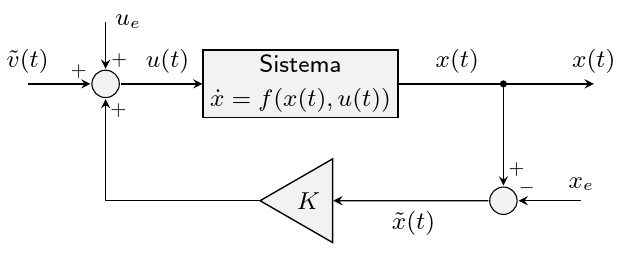
\includegraphics[scale=0.4]{Images/Controllo_retroazionato.png}
\end{center}
 




\section{Trasformata di Laplace}
\subsection{Definizione}
Data una funzione complessa $f$ di variabile reale $t$, $f: \mathbb{R} \rightarrow \mathbb{C}$ (anche se per noi tipicamente saranno funzioni $f: \mathbb{R} \rightarrow \mathbb{R}$), sia $s = \sigma + j \omega$ una variabile complessa ($\sigma$ parte reale, $\omega$ parte immaginaria); definiamo la \textit{Trasformata di Laplace} di $f(t)$
\begin{equation}
    F(s) = \int_{0^-}^{+ \infty} f(t) e^{-st} \ dt
\end{equation}
se esiste per qualche $s$, ovvero se l'integrale converge.\\
Includiamo nell'integrale $0^{-}$ per tener conto di eventuali impulsi cone la \textit{delta di Dirac}.
\vspace*{0.2cm}\\
\textbf{Notazione:} indichiamo la trasformata di Laplace con $\mathcal{L}$ tale che
\begin{equation}
    f(t) \overset{\mathcal{L}}{\xrightarrow{\hspace*{0.8cm}}} F(s)
\end{equation}
con $F:\mathbb{C} \rightarrow \mathbb{C}$; indichiamo l'applicazione della trasformata con $F(s) = \mathcal{L}[f(t)]$.


\subsection{Osservazioni}
\subsubsection{Ascissa di convergenza}
Sia $\overline{\sigma}>- \infty$ estremo inferiore di $s=\sigma + j \omega$ per cui l'integrale converge. Allora la trasformata di Laplace esiste nel semipiano $\operatorname{Re} (s)>\overline{\sigma}$. $\overline{\sigma}$ viene chiamata \textit{ascissa di convergenza}.\\
La trasformata di Laplace risulta essere una \textit{funzione analitica} e, grazie alle particolari proprietà delle funzioni analitiche, la sua definizione può essere estesa anche in punti $s$ tali che $ \operatorname{Re}(s)\leq \overline{\sigma}$, indipendentemente dal fatto che l'integrale non converga.
\vspace*{0.2cm}\\
Dato che 
\begin{equation}
    e^{-st} = e^{- \sigma t}e^{-j \omega t}
\end{equation}
possiamo dire che $e^{-\sigma t}$ ci aiuta a ottenere un integrale che converge.
\begin{center}
    \begin{tikzpicture}
            \begin{axis}[
                xmin=0,xmax=5,
                ymin=0,ymax=1,
                ticks=none, %elimina i valori numerici
                axis x line=middle,
                axis y line=middle,
                xlabel={$x$},
                ylabel={$y$},
                ]
                \addplot[domain=0.05:4.5, samples=100]{exp(-x)}node [pos=0.1,anchor=south west]{$e^{-\sigma t}$};
            \end{axis}
        \end{tikzpicture}
    \end{center}
\subsubsection{Trasformate razionali}
Di particolare importanza sono le \textit{trasformate razionali}, cioè quelle in cui
\begin{equation}
    F(s) = \frac{N(s)}{D(s)}
\end{equation}
con $N(s)$ e $D(s)$ polinomi primi tra loro. Le radici di $N(s)=0$ si dicono \textbf{zeri} e quelle di $D(s)=0$ si dicono \textbf{poli}: nell'insieme, poli e zeri si dicono \textit{singolarità}.
\vspace*{0.1cm}\\
Se $f$ è reale allora i coefficienti dei polinomi $N(s)$ e $D(s)$ sono reali.

\subsubsection*{Esempio}
\begin{equation}
    F(s) = \frac{s^2+2s}{(s+1)(s+3)} = \frac{s(s+2)}{(s+1)(s+3)}
\end{equation}
allora
\begin{itemize}
    \item zeri di $F(s)$: $0$ e $-2$
    \item poli di $F(s)$: $-1$ e $-3$
\end{itemize}


\subsection{Formula di antitrasformazione}
La funzione trasformanda può essere ricavata dalla sua trasformata
mediante la \textit{formula di antitrasformazione}
\begin{equation}
    f(t) = \frac{1}{2 \pi j} \int _{\sigma-j \infty}^{\sigma+j \infty} F(s) e^{st} \ ds
\end{equation}
\textbf{Notazione:} indichiamo l'antitrasformata di Laplace con $\mathcal{L}^{-1}$ tale che
\begin{equation}
    F(s) \overset{\mathcal{L}^{-1}}{\xrightarrow{\hspace*{0.8cm}}} f(t) \tag*{$\sigma > \overline{\sigma}$}
\end{equation}
indichiamo la formula di antitrasformazione con $f(t) = \mathcal{L}^{-1}[F(s)]$.
\vspace*{0.2cm}\\
La $f(t)$ è fornita per $t\geq 0$, perché solo nei punti di continuità in cui la $f$ è maggiore di zero essa contribuisce a determinare $F$. L'antitrasformata fornisce $f(t)=0$ per $t<0$, per questo la corrispondenza tra $f(t)$ e $F(s)$ è \textbf{biunivoca}.


\subsubsection{Perché si utilizza la trsformata di Laplace}
\begin{center}
    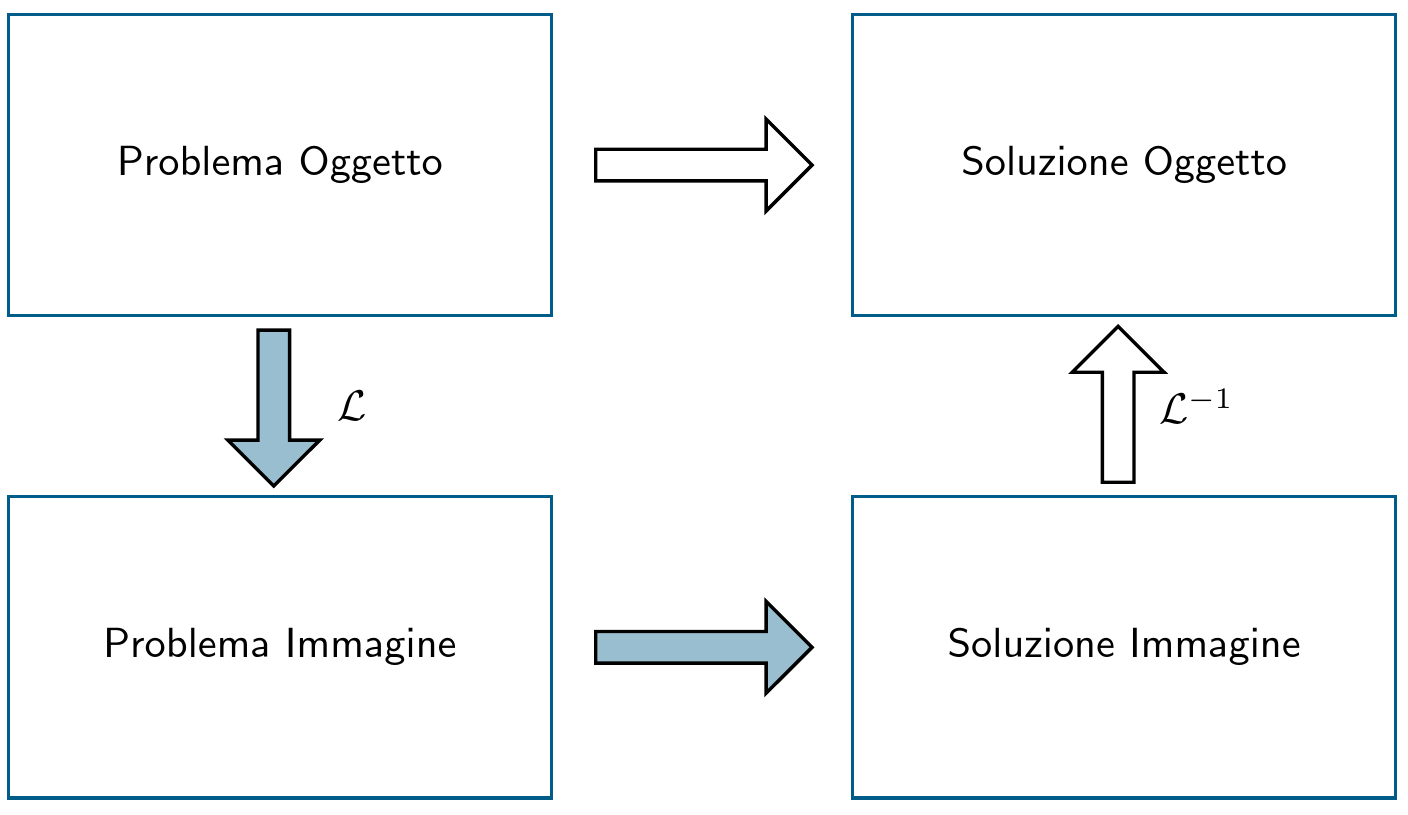
\includegraphics[scale=0.18]{Images/Motivo_Laplace.png}
\end{center}
Se, provando a risolvere il problema oggetto, risulta difficile arrivare alla soluzione oggetto (magari perché i calcoli sono molto complessi o risulta poco conveniente in termini di risorse), allora si trasforma il problema oggetto in problema immagine con la trasformata di Laplace se risulta poi conveniente (o semplice) arrivare alla soluzione immagine, per poi antitrasformarla per ottenere la soluzione oggetto che si stava cercando.


\subsection{Proprietà della trasformata di Laplace}
\subsubsection{Linearità}
Dati $f(t)$ e $g(t)$ tali per cui esistono le trasformate $F(s)$ e $G(s)$, allora $\forall \alpha \in \mathbb{C}, \forall \beta \in \mathbb{C}$ risulta
\begin{equation}
    \mathcal{L}[\alpha f(t) + \beta g(t)] = \alpha \mathcal{L}[f(t)] + \beta \mathcal{L}[g(t)] = \alpha F(s) + \beta G(s)
\end{equation}

\subsubsection*{Dimostrazione}
\begin{align*}
    \mathcal{L}[\alpha f(t) + \beta g(t)] &= \int_{0^{-}}^{+\infty}\left(\alpha f(t) + \beta g(t)\right) e^{-st} \ dt\\
    &= \alpha \underbrace{\int_{0^{-}}^{+\infty} f(t)e^{-st} \ dt}_{F(s)} + \beta \underbrace{\int_{0^{-}}^{+\infty} g(t)e^{-st} \ dt}_{G(s)}\\
    &= \alpha F(s) + \beta G(s)
\end{align*}

\subsubsection{Traslazione temporale}
\begin{equation}
    \mathcal{L}[f(t-\tau)] = e^{-\tau s}F(s) \tag*{$\forall \tau >0$}
\end{equation}
$\tau$ deve essere maggiore di 0, altrimenti la $f(t)$ sarebbe diversa da 0 per un tempo negativo.

\subsubsection*{Dimostrazione}
\begin{align*}
    \mathcal{L}[f(t-\tau)] &= \int_{0^-}^{+ \infty} f(t - \tau)e^{-st} \ dt\\
    &\underset{\rho = t-\tau}{=} \int_{-\tau^-}^{+ \infty} f(\rho)e^{-s(\rho+t)} \ d\rho\\
\end{align*}
siccome la $f(t)$ è nulla per $t<0$ posso riscrivere gli estremi di integrazione
\begin{align*}
    \int_{0^-}^{+ \infty} f(\rho)e^{-s(\rho+t)} \ d\rho
    &= \underbrace{\int_{0^-}^{+ \infty} f(\rho)e^{\rho} \ d\rho}_{F(s)} \cdot e^{-s\tau} \\
    &= F(s) e^{-s\tau}
\end{align*}
come volevasi dimostrare
\begin{equation}
    \mathcal{L}[f(t-\tau)] = e^{-\tau s}F(s)
\end{equation}

\subsubsection{Traslazione nel dominio della variabile complessa}\label{Traslazione nel dominio della variabile complessa}
\begin{equation}
    \mathcal{L}[e^{\alpha t }f(t)] = F(s - 
    \alpha)
\end{equation}

\subsubsection*{Dimostrazione}
\begin{align*}
    \mathcal{L}[e^{\alpha t }f(t)] &= \int_{0^-}^{+ \infty} f(t)e^{\alpha t} \cdot e^{-st} \ dt \\
    &= \int_{0^-}^{+ \infty} f(t)e^{-(s-\alpha)t} \ dt\\
    &= F(s-\alpha)
\end{align*}

\subsubsection{Derivazione nel dominio del tempo}\label{Derivazione nel dominio del tempo}
\begin{equation}
    \mathcal{L}\left[\frac{d}{dt}f(t)\right] = sF(s) - f(0)
\end{equation}
Calcoliamo la trasformata della derivata seconda
\begin{align*}
    \mathcal{L}\left[\frac{d^2}{dt^2}f(t)\right] &=
    \mathcal{L}\left[\frac{d}{dt}\underbrace{\left[\frac{d}{dt}f(t)\right]}_{g(t)}\right]\\
    &=sG(s) - g(0)\\
    &=sG(s) - f'(0)\\
    &=s(sF(s)-f(0)) - f'(0)\\
    &= s^2 F(s) - sf(0) - f'(0)
\end{align*}
Quindi possiamo definire la \textit{derivata n-sima nel tempo}
\begin{equation}
    \mathcal{L}\left[\frac{d^n}{dt^n}f(t)\right] = s^nF(s) = \sum_{i=1}^n s^{n-i} \frac{d^{i-1}}{dt^{i-1}}f(t)|_{t=0}
\end{equation}
La proprietà ci dice che, se la funzione e le sue derivate si annullano in $t=0$, derivare nel dominio del tempo equivale a moltiplicare per $s$ nel dominio della variabile complessa; infatti $s$ viene chiamato \textit{operatore di derivazione}.


\subsubsection{Derivazione nel dominio della variabile complessa}\label{Derivazione nel dominio della variabile complessa}
Supponiamo $F(s)$ derivabile per tutti gli $s$; allora risulta
\begin{equation}
    \mathcal{L}[t f(t)] = - \frac{dF(s)}{ds}
\end{equation}
la quale è estendibile al caso della trasformata $t^n \cdot f(t)$.

\subsubsection*{Dimostrazione}
Considerando che $te^{-st} = -\dfrac{d}{ds}e^{-st}$
\begin{align*}
    \mathcal{L}[t f(t)] &= \int_{0^+}^{+\infty} t f(t)e^{-st} \ dt\\
    &=\int_{0^+}^{+\infty} f(t) \underbrace{te^{-st}}_{-\frac{d}{ds}e^{-st}} \ dt\\
    &=\int_{0^+}^{+\infty} f(t) \left(-\frac{d}{ds}e^{-st}\right) \ dt\\
    &=-\frac{d}{ds} \underbrace{\int_{0^+}^{+\infty} f(t) e^{-st} \ dt}_{F(s)}\\
    &= - \frac{dF(s)}{ds}
\end{align*}


\subsubsection{Integrazione nel tempo}
Supponiamo che la funzione $f(t)$ sia integrabile tra 0 e $+ \infty$. Allora
\begin{equation}
    \mathcal{L} \left[\int_0^tf(\tau) \ d\tau\right] = \frac{1}{s} F(s)
\end{equation}
La proprietà ci dice che integrare nel dominio del tempo equivale a dividere per $s$ nel dominio della variabile complessa; infatti $\dfrac{1}{s}$ viene chiamato \textit{operatore di integrazione}.


\subsubsection{Convoluzione nel tempo}
Date due funzioni $f_1$ e $f_2$, il loro \textit{prodotto di convoluzione} è
\begin{equation}
    f_1(t) \ast f_2(t) = \int_{-\infty}^{+\infty} f_1(t -\tau)f_2(t) \ d\tau = \int_{-\infty}^{+\infty} f_1(\eta)f_2(\eta) \ d\eta = f_2(t-\eta) \ast f_1(t)
\end{equation}
e si trova
\begin{equation}
    \mathcal{L}[f_1(t) \ast f_2(t)] = F_1(s) \cdot F_2(s)
\end{equation}

\subsubsection{Teorema del valore iniziale}
Se una funzione reale $f(t)$ ha trasformata razionale $F(s)$ con grado del denominatore maggiore del grado del numeratore, allora
\begin{equation}
    f(0) = \lim_{s\rightarrow \infty} s F(s)
\end{equation}
Se $f$ è una funzione discontinua di prima specie in $t=0$, $f(0)$ si interpreta come $f(0^+)$. L'equazione vale se $f(0)$ o $f(0^+)$ esistono.


\subsubsection{Teorema del valore finale}
Se una funzione reale $f(t)$ ha trasformata razionale $F(s)$ con grado del denominatore maggiore del grado del numeratore e poli nulli o con parte reale negativa, allora
\begin{equation}
    \lim_{t \rightarrow + \infty} f(t) = \lim_{s\rightarrow 0} s F(s)
\end{equation}
L'equazione vale se esiste $\lim\limits_{t \rightarrow + \infty}f(t)$ esiste.


\subsection{Trasformata di segnali elementari}
Definiamo il \textit{delta di Dirac} $\delta(t)$ tale che
\begin{equation}
    \int_{0^-}^{0^+} \delta(t) \ dt = 1
\end{equation}
\begin{center}
    \renewcommand{\arraystretch}{5}
    \begin{tabular}{c c}
        $\mathcal{L}[\delta(t)]=1$ & 
        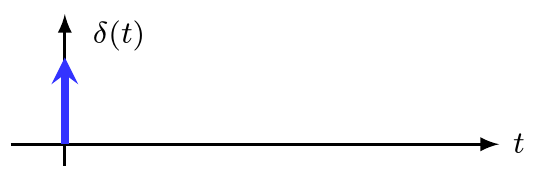
\includegraphics[width=0.25\linewidth, valign=c]{Images/Delta.png}
        \\
        $\mathcal{L}[1(t)]=\dfrac{1}{s}$ & 
        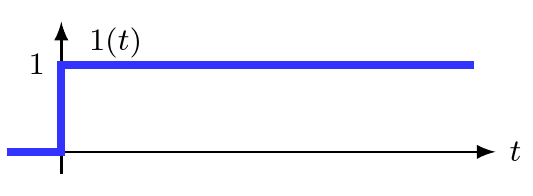
\includegraphics[width=0.25\linewidth, valign=c]{Images/Scalino.png}
        \\
        $\mathcal{L}[t \cdot 1(t)]=\dfrac{1}{s^2}$ & 
        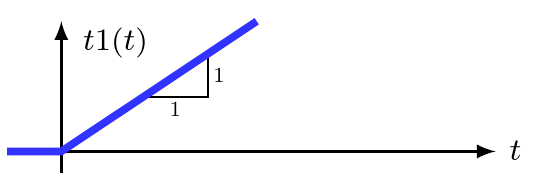
\includegraphics[width=0.25\linewidth, valign=c]{Images/Scalino_2.png}
        \\
        $\mathcal{L}[e^{\alpha t} \cdot 1(t)]=\dfrac{1}{s-\alpha}$ & 
        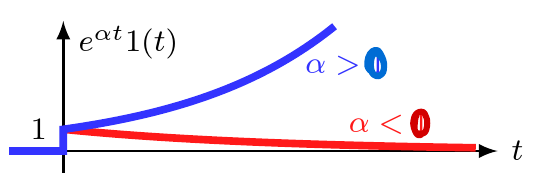
\includegraphics[width=0.25\linewidth, valign=c]{Images/Scalino_3.png}\\
    \end{tabular}
\end{center}

\subsubsection{Trasformata della delta}
\begin{align*}
    \mathcal{L}[\delta(t)] &= \int_{0^-}^{+\infty} \delta(t) e^{-st} \ dt \\
    &= \int_{0^-}^0 \delta(t) \underbrace{e^{-s\cdot 0}}_{1} \ dt + \underbrace{\int_{0^+}^{+\infty} \underbrace{\delta(t)}_{0} e^{-st} \ dt}_{0} \\
\end{align*}

\subsubsection{Trasformata del segnale gradino unitario}
Il segnale gradin unitario $1(t)$ è definito
\begin{equation}
    1(t) = \begin{cases}
        0 &t<0\\
        1 &t\geq 0
    \end{cases}
\end{equation}
\begin{align*}
    \int_{0^-}^{+ \infty} 1(t)e^{-st} \ dt &= \int_{0}^{+ \infty} \underbrace{1(t)}_{1}e^{-st} \ dt\\
    &= \int_{0}^{+ \infty}e^{-st} \ dt\\
    &= \frac{e^{-st}}{-s}\bigg|_{t\rightarrow+\infty} - \frac{e^{-0}}{-s}\bigg|_{t=0}
\end{align*}
$\lim_{t\rightarrow+\infty}e^{-st}=0$, $e^0=1$
\begin{equation}
    \underbrace{\frac{\overbrace{e^{-st}}^{0}}{-s}}_{0}\bigg|_{t\rightarrow+\infty} - \frac{\overbrace{e^{-0}}^{1}}{-s}\bigg|_{t=0} = \frac{1}{s}
\end{equation}

\subsubsection{Trasformata del segnale rampa}
Il segnale \textit{rampa} $r(t)$ è definito come
\begin{equation}
    r(t) = \begin{cases}
        0 &t<0\\
        t &t\geq 0
    \end{cases} \ \ \ \ \  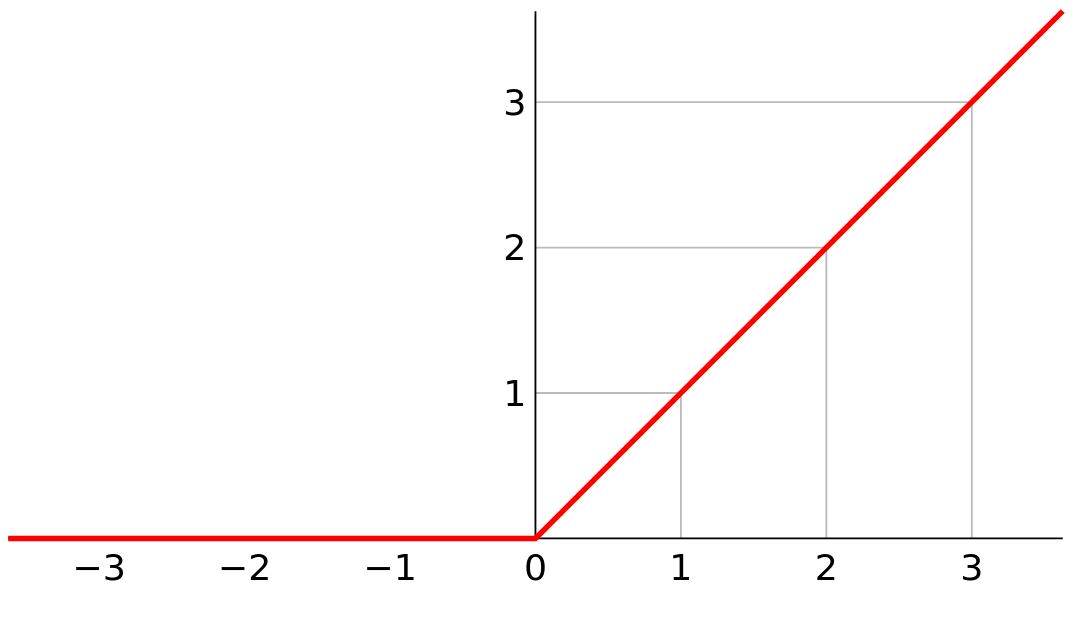
\includegraphics[width=0.25\linewidth, valign=c]{Images/Segnale_rampa.png}
\end{equation}
Per calcolare la trasformata del segnale rampa utilizziamo la proprietà di \nameref{Derivazione nel dominio della variabile complessa}
\begin{align*}
    \mathcal{L}[t \cdot 1(t)] &= -\frac{d\left(\dfrac{1}{s}\right)}{ds}\\
    &= \frac{1}{s^2}
\end{align*}
\vspace*{0.2cm}\\
Mentre per calcolare la trasformata del gradino moltiplicato un esponenziale utilizziamo la proprietà di \nameref{Traslazione nel dominio della variabile complessa}
\begin{align*}
    \mathcal{L}[e^{\alpha t} \underbrace{1(t)}_{f(t)}] &= \underbrace{F(s-\alpha)}_{F(s)=\frac{1}{s}}\\
    &= \frac{1}{s-\alpha}
\end{align*}

\subsection{Tabella delle trasformate}\label{Tabella delle trasformate}

\begin{center}
    \renewcommand{\arraystretch}{5}
    \begin{tabular}{c c}
        $\mathcal{L}[\delta(t)]=1$ & 
        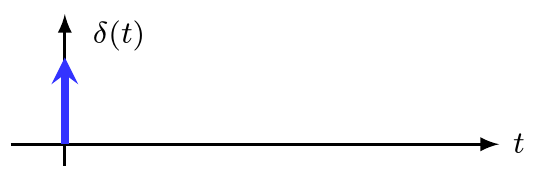
\includegraphics[width=0.25\linewidth, valign=c]{Images/Delta.png}
        \\
        $\mathcal{L}[1(t)]=\dfrac{1}{s}$ & 
        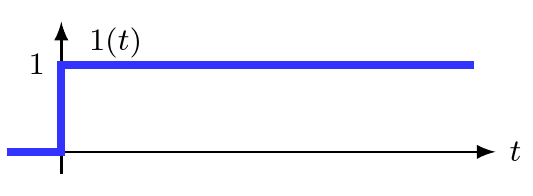
\includegraphics[width=0.25\linewidth, valign=c]{Images/Scalino.png}
        \\
        $\mathcal{L}[t \cdot 1(t)]=\dfrac{1}{s^2}$ & 
        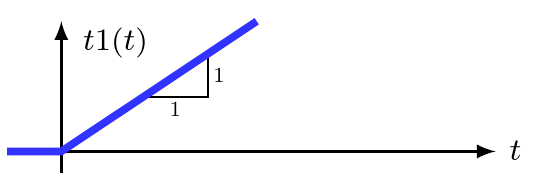
\includegraphics[width=0.25\linewidth, valign=c]{Images/Scalino_2.png}
        \\
        $\mathcal{L}[e^{\alpha t} \cdot 1(t)]=\dfrac{1}{s-\alpha}$ & 
        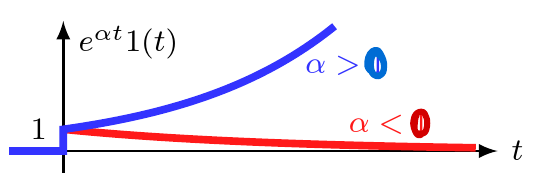
\includegraphics[width=0.25\linewidth, valign=c]{Images/Scalino_3.png}\\
        $\mathcal{L}[\sin(\omega t)1(t)]= \dfrac{\omega}{s^2+\omega^2}$ & 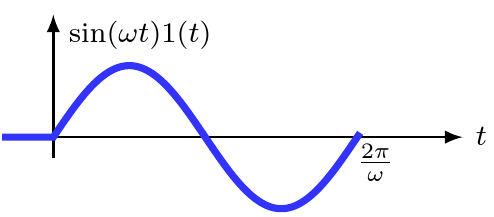
\includegraphics[width=0.25\linewidth, valign=c]{Images/Trasformata_seno.png}\\
        $\mathcal{L}[\cos(\omega t)1(t)]= \dfrac{\omega}{s^2+\omega^2}$ & 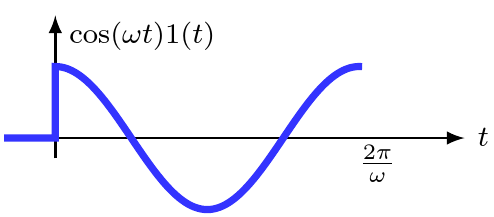
\includegraphics[width=0.25\linewidth, valign=c]{Images/Trasformata_coseno.png}\\
        $\mathcal{L}[\sin(\omega t + \varphi)1(t)]= \dfrac{\omega \cos\varphi \pm s \sin\phi}{s^2+\omega^2}$\\
        $\mathcal{L}[\cos(\omega t + \varphi)1(t)]= \dfrac{s \cos\phi \mp \omega \sin\varphi}{s^2+\omega^2}$
    \end{tabular}
\end{center}



\section{Funzione di trasferimento}
\subsection{Introduzione}
Consideriamo il sistema LTI con $x\in \mathbb{R}^n, u\in \mathbb{R}^m,y\in \mathbb{R}^p$
\begin{align*}
    \dot x(t) &= Ax(t) + Bu(t)\\
    y(t) &= Cx(t) + Du(t)
\end{align*}
con $x(0) = x_0$.
\vspace*{0.1cm}\\
Siano $X(s):= \mathcal{L}[x(t)], U(s):= \mathcal{L}[u(t)]$ e $Y(s):= \mathcal{L}[y(t)]$. Applichiamo la trasformazione di Laplace ad ambo i membri delle equazioni precedenti, ricordando che $\mathcal{L}\left[\dfrac{d}{dt}x(t)\right]=sX(s)-x(0)$
\begin{align*}
    sX(s) - x(0) &= AX(s) + BU(s)\\
    Y(s) &= CX(s) + DU(s) 
\end{align*}
se raccolgo $X(s)$ nella prima equazione
\begin{align*}
    (sI-A)X(s) &=x_0+ BU(s)\\
    Y(s) &= CX(s) + DU(s) 
\end{align*}
\begin{align*}
    X(s) &=\overbrace{(sI-A)^{-1}x_0}^{X_\ell (s)} +\overbrace{(sI-A)^{-1} BU(s)}^{X_f (s)}\\
    Y(s) &= CX(s) + DU(s) 
\end{align*}
Sottolineiamo che se avessimo un sistema generico non si potrebbe riscrivere come abbiamo fatto perché \underline{le matrici devono essere} \underline{costanti}.\\
Inoltre per poter scrivere un sistema LTI come sopra la matrice $(sI-A)$ deve essere invertibile; una matrice è invertibile se il suo determinante è non nullo, quindi, se $s$ è autovalore della matrice della dinamica e $p(s)$ è il polinomio caratteristico associato:
\begin{equation}
    p(s) = \det (sI-A)
\end{equation}
Quindi le trasformate dello stato e dell'uscita del sistema in funzione di $x_0$ e $U(s)$ sono 
\begin{align*}
    X(s) &=\overbrace{(sI-A)^{-1}x_0}^{\T{evoluzione libera}} +\overbrace{(sI-A)^{-1} BU(s)}^{\T{evoluzione forzata}}\\
    Y(s) &=\underbrace{C(sI-A)^{-1}x_0}_{\T{evoluzione libera}} + \underbrace{\left(C(sI-A)^{-1}B+D\right)U(s)}_{\T{evoluzione forzata}}
\end{align*}
\begin{align*}
    X_\ell(s) &= (sI-A)^{-1}x_0 & X_f(s) &= (sI-A)^{-1} BU(s)\\
    Y_\ell(s) &= C(sI-A)^{-1}x_0 & Y_f(s) &= \left(C(sI-A)^{-1}B+D\right)U(s)  
\end{align*}
Consideriamo ora la trasformata dell'evoluzione forzata dell'uscita
\begin{equation*}
    Y_f(s) = \left(C(sI-A)^{-1}B+D\right) U(s)
\end{equation*}
la matrice
\begin{equation*}
    G(s) = C(sI-A)^{-1}B+D
\end{equation*}
è detta \textit{funzione di trasferimento}; se il sistema è SISO (Single Input Single Output) è una funzione scalare.
\vspace*{0.1cm}\\
Abbiamo così ottenuto una \textbf{rappresentazione ingresso-uscita}
\begin{equation}
    Y_f(s) = G(s)U(s)
\end{equation}
se assumiamo che $x(0)=0$ otteniamo esattamente la trasformata di Laplace dell'uscita $y$
\begin{equation}\label{funzione di trasferimento}
    Y(s) = G(s)U(s)
\end{equation}
Due osservazioni:
\begin{itemize}[label=$\triangleright$]
    \item se si conosce la funzione di trasferimento $G(s)$ di un sistema e la trasformata di Laplace $U(s)$ dell'ingresso, è possibile calcolare, mediante antitrasformazione dell'equazione precedente \ref{funzione di trasferimento}, il movimento forzato $y_f$ dell'uscita (che ovviamente coincide con il movimento $y$ se lo stato iniziale è nullo);
    \item la funzione di trasferimento è data dal rapporto tra la trasformata dell'uscita e dell'ingresso nel caso di $x(0)=0$
    \begin{equation}
        G(s) = \frac{Y(s)}{U(s)}
    \end{equation}
\end{itemize}

\subsection{Richiami di calcolo matriciale}

\subsubsection{Matrice diagonale}
Una \textit{matrice diagonale} è una matrice quadrata tale che per $i \neq j$ si ha sempre $a_{ij}=0$ (ogni matrice diagonale è simmetrica).
$$ \begin{pmatrix} 1&0&0&0 \\ 0&7&0&0 \\ 0&0&9&0 \\ 0&0&0&-3  \end{pmatrix}, \ \begin{pmatrix} 0&0&0&0 \\ 0&2&0&0 \\ 0&0&3&0 \\ 0&0&0&1  \end{pmatrix} $$


\subsubsection{Matrice triangolare alta}
Una \textit{matrice triangolare alta} è una matrice quadrata tale che per $i>j \ \  a_{ij}=0$
$$ \begin{pmatrix} a_{11}&a_{12}&a_{13}&a_{14} \\ a_{21}&a_{22}&a_{23}&a_{24} \\ a_{31}&a_{32}&a_{33}&a_{34} \\ a_{41}&a_{42}&a_{43}&a_{44} \end{pmatrix} \rightarrow \begin{pmatrix} 1&4&-3&7 \\ 0&6&-8&9\\ 0&0&3&-5 \\ 0&0&0&1 \end{pmatrix}   $$


\subsubsection{Matrice triangolare bassa}
Una \textit{matrice triangolare alta} è una matrice quadrata tale che per $i<j \ \  a_{ij}=0$
$$ \begin{pmatrix} a_{11}&a_{12}&a_{13}&a_{14} \\ a_{21}&a_{22}&a_{23}&a_{24} \\ a_{31}&a_{32}&a_{33}&a_{34} \\ a_{41}&a_{42}&a_{43}&a_{44} \end{pmatrix} \rightarrow \begin{pmatrix}  1&0&0&0 \\ 6&7&0&0 \\ 3&-2&-9&0 \\ 5&4&-8&3 \end{pmatrix}   $$
Nota: una matrice diagonale è triangolare alta e triangolare bassa.


\subsubsection{Matrice identità}
$$ I_n = \begin{pmatrix}
1 & 0 & .. & 0\\
0 & .. & .. & .. \\
.. & .. & .. & ..  \\
0 & .. & .. & 1
\end{pmatrix} I_2 = \begin{pmatrix} 1 & 0 \\ 0 & 1 \end{pmatrix} $$


\subsubsection{Trasposta di una matrice}
$$\begin{pmatrix}
2 & 1 & 7 \\
4 & 0 & 2
\end{pmatrix}^T = \begin{pmatrix}2 & 4 \\ 1 & 0 \\ 7 & 2 \end{pmatrix} $$
$A = (a_{ij})$ significa che l'elemento di posto $(i,j)$ in $A$ è $a_{i,j}$.
\vspace{0.2cm}\\
$A^T := B = (b_{ij})$ con $b_{ij} = a_{ji}$ per ogni coppia di indici $(i,j)$.


\subsubsection{Complemento algebrico}
Definiamo $\hat A_{ij}$ complemento algebrico dell'elemento $a_{ij}$ il determinante della matrice ottenuta eliminando da $A$ la riga $i$ e la colonna $j$ (che chiamiamo $M$) e moltiplicando per $(-1)^{i+j}$
\begin{equation*}
    \hat A_{ij} = (-1)^{i+j} \det(M)
\end{equation*}


\subsubsection{Determinante di una matrice}
Il determinante di una matrice generica si calcola
\begin{equation*}
    det(A) = \sum_{i=1}^n a_{ij} \hat A_{ij} = \sum_{j=1}^n a_{ij} \hat A_{ij}
\end{equation*}



\subsection{Funzione di trasferimento nel dettaglio}
La funzione di trasferimento è definita
\[
    G(s) = C(sI-A)^{-1}B + D
\]
con $C$ matrice $1 \times n$ e $B$ matrice $m \times 1$.
\vspace*{0.2cm}\\
Definiamo ora la \textbf{matrice aggiunta} $\T{adj}(A)$ come matrice dei complementi algebrici di $A$
\begin{equation}
    \T{adj}(A) = 
    \begin{bmatrix}
        \hat A_{11} & \hat A_{12} & \cdots & \hat A_{n1} \\
        \hat A_{12} & \hat A_{22} & \dots & \hat A_{n2} \\
        \vdots & \vdots  & \ddots & \vdots\\
        \hat A_{n1} & \hat A_{n2} & \dots & \hat A_{nn}
    \end{bmatrix}
\end{equation}
La matrice inversa può essere definita con la matrice aggiunta:
\begin{equation}
    A^{-1} = \frac{\T{adj}(A)}{\det(A)}
\end{equation}
Quindi, se consideriamo la nostra matrice $(sI-A)$
\begin{equation}
    (sI-A)^{-1} = \frac{\T{adj}(sI-A)}{\underbrace{\det(sI-A)}_{\substack{\text{polinomio} \\ \text{caratteristico di } A}}}
\end{equation}
quindi scriviamo la matrice aggiunta di $(sI-A)$
\begin{equation}
    \T{adj}(sI-A) = 
    \begin{bmatrix}
        \widehat{(sI-A)}_{11} & \widehat{(sI-A)}_{12} & \cdots &  \widehat{(sI-A)}_{n1} \\
        \widehat{(sI-A)}_{12} & \widehat{(sI-A)}_{22} & \dots & \widehat{(sI-A)}_{n2} \\
        \vdots & \vdots  & \ddots & \vdots\\
        \widehat{(sI-A)}_{n1} & \widehat{(sI-A)}_{n2} & \dots & \widehat{(sI-A)}_{nn}
    \end{bmatrix}
\end{equation}
matrice di polinomi in $s$ al più di grado $n-1$; il determinante di $sI-A$ è un polinomio in $s$ di grado $n$. Per cui 
\begin{equation}
    (sI-A)^{-1} = \underbrace{\frac{1}{\det(sI-A)}}_{\T{scalare}} \cdot \T{adj}(sI-A)
\end{equation}
Allora possiamo scrivere la funzione di trasferimento come
\begin{equation}
    G(s) = \frac{\overbrace{N_{sp}(s)}^{\substack{\text{polinomio di } \\ \text{grado al più } n-1}}}{\underbrace{D_{sp}(s)}_{\substack{\text{polinomio} \\ \text{di grado } n}}} 
    + \underbrace{D}_{\substack{\text{polinomio non} \\ \text{strettamente} \\ \T{proprio}}}
\end{equation}
in forma estesa:
\begin{equation}
    G(s) = \frac{N(s)}{D(s)} = \frac{\beta_{\nu}s^{\nu} + \beta_{\nu-1}s^{\nu-1} + \cdots + \beta_1s + \beta_0}{s^{\nu}\footnotemark + \alpha_{\nu-1}s^{\nu-1} + \cdots + \alpha_1s + \alpha_0}
\end{equation}
\footnotetext{trasformata della delta di Dirac}
Le radici di $N(s)$ si dicono \textbf{zeri}, le radici di $D(s)$ si dicono \textbf{poli}; i poli sono radici di $\det(sI-A)$ quindi sono autovalori di $A$. Poli e zeri sono reali o complessi coniugati, poiché radici di polinomi a coefficienti reali.

\subsubsection*{Esempio 1}
Se prendiamo $y(t) = \dfrac{d}{dt} u(t)$, allora la sua trasformata sarà $Y(s)=s U(s)$, quindi la funzione di trasferimento del sistema è $G(s)=s$; il sistema non è causale, perché il grado del numeratore ha grado maggiore di quello del denominatore. Questa considerazione diventa evidente se si utilizza la definizione di derivata:
\[
    y(t) = \frac{d}{dt}(u(t)) = \lim_{h\rightarrow 0} \frac{u(t+h)-u(t)}{h}
\]
infatti per conoscere la derivata in $t$ devo conoscere il valore del segnale in $t+h$.

\subsubsection*{Esempio 2}
\begin{align*}
    y(t) &= \int_{0}^t u(\tau) \ dt & Y(s) &= \frac{1}{s}U(s)
\end{align*}



\subsection{Schema dell'utilizzo della trasformata di Laplace}
\begin{center}
    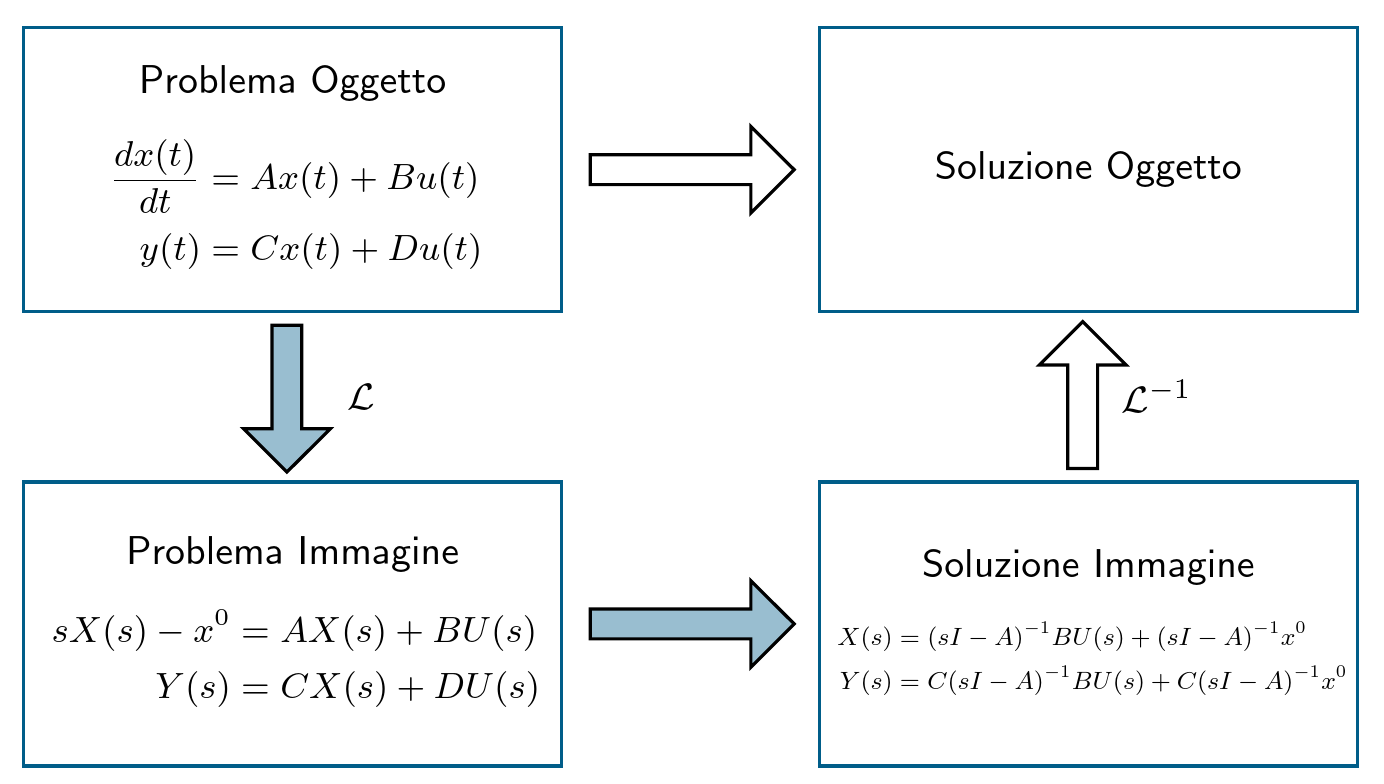
\includegraphics[scale=0.25]{Images/Schema_trasformata.png}
\end{center}


\subsection{Rappresentazioni e parametri della funzione di trasferimento}\label{Rappresentazioni e parametri della funzione di trasferimento}
Può essere conveniente, in alcune situazioni, rappresentare la funzione di trasferimento in una delle seguenti forme fattorizzate
\begin{equation}\label{parametrizzazione 1}
    G(s) = \frac{\rho \prod_i (s + z_i)\prod_i (s^2+2 \zeta_i \alpha_{ni}s  +\alpha^2_{ni})}
                {s^g \prod_i (s + p_i)\prod_i (s^2+2 \xi_i \omega_{ni}s + \omega^2_{ni})}
\end{equation}
\begin{equation}\label{Forma di bode}
    G(s) = \frac{\mu \prod_i (1 + \tau_i s)\prod_i (1 + \frac{2\zeta_i}{\alpha_{ni}} + \frac{s^2}{\alpha^2_{ni}})}
                {s^g \prod_i (1 + T_i s)\prod_i (1 + \frac{2\xi_i}{\omega_{ni}} + \frac{s^2}{\omega^2_{ni}})}
\end{equation}
\textbf{N.B.} il pedice $n$ sta per "naturale".
Con 
\begin{itemize}
    \item lo scalare $\rho$ è detto costante di trasferimento, $\mu$ il \textit{guadagno};
    \item l'intero $g$ è detto \textit{tipo};
    \item gli scalari $-z_i$ e $-p_i$ sono gli zeri e i poli reali non nulli;
    \item gli scalari $\alpha_{ni} > 0$ e$\omega_{ni} > 0$ sono le \textit{pulsazioni naturali} delle coppie di zeri e poli complessi coniugati;
    \item gli scalari $\zeta_i$ e $\xi_i$, in modulo minori di 1, sono gli \textit{smorzamenti} degli zeri e dei poli complessi coniugati;
    \item gli scalari $\tau_i \neq 0$ e $T_i \neq 0$ sono le costanti di tempo
\end{itemize}
La seconda equazione (\ref{Forma di bode}) è detta \textit{forma di Bode}.

\subsubsection{Esempio}
\[
    G(s) = 10 \cdot \frac{\overbrace{s+10}^{\prod_i(s+z_i)}}{s^2(s+1)(s+100)}
\]
\begin{align*}
    z_1 &= 10 & p_1 &= 1 \\
    & & p_2 &= 100\\
    \rho &= 10 & g &= 2
\end{align*}
C'è un solo zero, che è $-10$, mentre i poli sono $0,-1,-100$.
\vspace*{0.2cm}\\
Scriviamo la funzione di trasferimento nella seconda forma (di Bode):
\[
    G(s) = \frac{\cancel{10}}{s^2} \cdot \frac{\cancel{10} \cdot \left(1 + \dfrac{s}{10}\right)}{\cancel{100}(1+s)\left(1 + \dfrac{s}{100}\right)} = 1\cdot \frac{(1 + 0.1 s)}{s^2(1+s)(1+10^{-2}s)}
\]
\begin{align*}
    \mu &= 1 & \tau_1 &= 0.1\\
    T_1 &= 1 & T_2 &= 10^{-2}
\end{align*}
Prendiamo un polinomio di II grado del denominatore
\[
    s^2 + 2 \xi_i \omega_{ni}s + \omega^2_{ni}
\]
le radici del polinomio sono:
\begin{align*}
    s_{1/2} &= - \xi_i\omega_{ni} \pm \sqrt{\xi_i^2\omega_{ni}^2 - \omega_{ni}^2}\\
    &=- \xi_i \omega_{ni} \pm \omega_{ni} \sqrt{\xi_i^2 - 1}
\end{align*}
Se $|\xi_i|<1$ abbiamo dei \textit{poli complessi coniugati}
\[
    s_{1/2} = - \xi_i \omega_{ni} + j \omega_{ni} \sqrt{1 - \xi_i^2}
\]
\begin{align*}
    |s_1| = |s_2| &= \sqrt{\xi_i^2 \omega_{ni}^2 + \omega_{ni}^2 (1 - \xi_i^2)}\\
    &= \sqrt{\xi_i^2 \omega_{ni}^2 + \omega_{ni}^2  - \omega_{ni}^2\xi_i^2}\\
    &= \omega_{ni}
\end{align*}
Rappresentiamo i poli nel piano complesso:
\begin{center}
    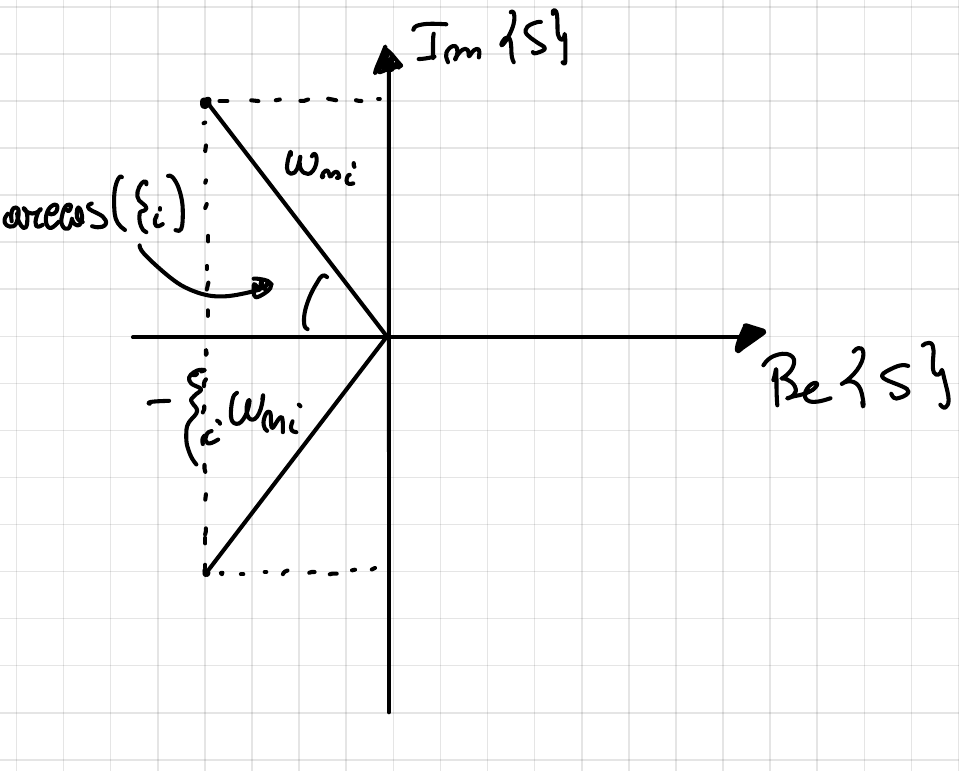
\includegraphics[scale=0.23]{Images/Poli_piano.png}
\end{center}
$\omega_{ni}$ quindi è il modulo delle radici, $\xi_i$ ci da invece informazioni sull'angolo delle radici nel piano complesso: se $\xi_i>0$ si hanno dei poli a parte reale negativa, se $\xi_i<0$ si hanno dei poli a parte reale positiva.\\
Se $\xi_i=0$ gli autovalori sono immaginari puri, quindi i modi del sistema sono sinusoidi non smorzate, dato che lo smorzamento è nullo.
\vspace*{0.2cm}\\
Nella rappresentazione classica si una una \textit{x} per i poli e un $\circ$ per gli zeri
\begin{center}
    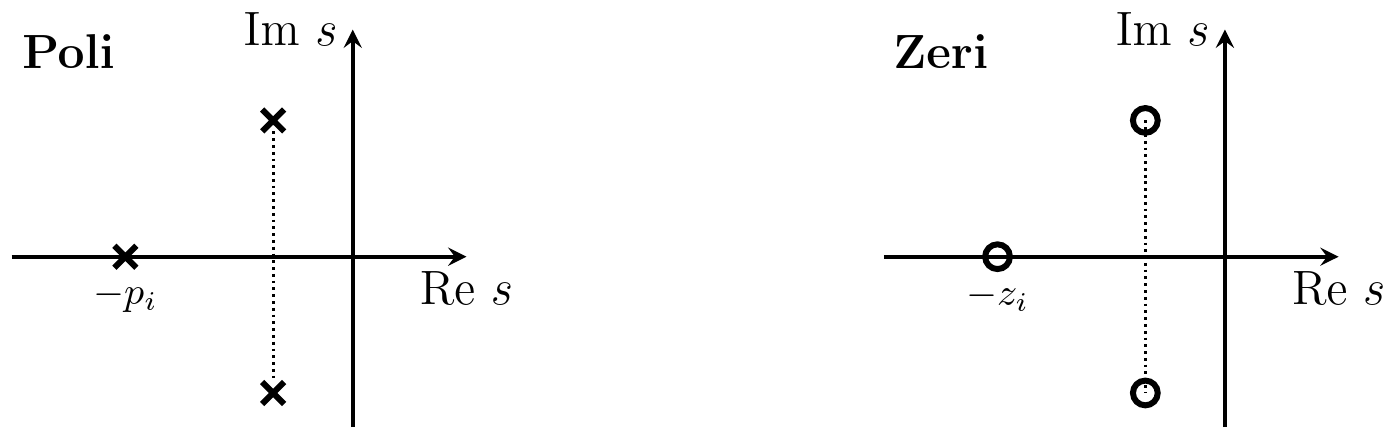
\includegraphics[scale=0.23]{Images/Poli_rapp_classica.png}
\end{center}


\subsection{Cancellazioni}
\subsubsection{Esempio 1}
\begin{align*}
    \dot x_1 &= -x_1 + x_2\\
    \dot x_2 &= -2x_2 + u\\
    y &= x_2
\end{align*}
\begin{align*}
    G(s)    &= C(sI-A)^{-1} B \\
            &=  \begin{bmatrix}
                0 & 1
                \end{bmatrix}
                \begin{bmatrix}
                    s+1 & -1\\
                    0   & s+2 
                \end{bmatrix}^{-1}
                \begin{bmatrix}
                    0 \\ 1
                \end{bmatrix}\\
            &= \begin{bmatrix}
                0 & 1
                \end{bmatrix}
                \begin{bmatrix}
                    \frac{s+2}{(s+1)(s+2)} & \frac{1}{(s+1)(s+2)}\\
                    0   & \frac{s+2}{(s+1)(s+2)}
                \end{bmatrix}^{-1}
                \begin{bmatrix}
                    0 \\ 1
                \end{bmatrix}
            \\
            &= \frac{\cancel{s+1}}{\cancel{(s+1)}(s+2)}\\
            &= \frac{1}{s+2}
\end{align*}
Guardando questo esempio ci verrebbe da pensare che le cancellazioni sono innocue, ma questo perché stiamo cancellando il polinomio associato a un autovalore reale negativo, che quindi fa convergere il mio sistema.

\subsubsection{Esmepio 2}
Se prendiamo invece un sistema di questo tipo
\begin{align*}
    \dot x_1 &= x_1 + x_2\\
    \dot x_2 &= x_2 + u\\
    y &= x_2
\end{align*}
la funzione di trasferimento di questo sistema è 
\[
    G(s) = \frac{\cancel{(s-1)}}{\cancel{(s-1)}(s+2)} = \frac{1}{s+2}
\]
In questo caso stiamo cancellando un polinomio associato a un autovalore reale positivo, che quindi fa \underline{divergere} il sistema, perciò bisogna stare attenti quando si eseguono cancellazioni. Non basta guardare la funzione di trasferimento per conoscere l'andamento del sistema.


\subsection{Antitrasformazione di Laplace}
Ricordiamo che la trasformata della risposta di un sistema Lineare Tempo Invariante (LTI) singolo ingresso singola uscita (SISO) è data da
\[
    Y(s) = C(sI-A)^{-1} x(0) + G(s)U(s)
\]
con $C(sI-A)^{-1} \in \mathbb{R}^{1 \times n}$. Si può far vedere che gli elementi di $C(sI-A)^{-1}$ sono rapporti di polinomi.\\
Nel corso della trattazione considereremo ingressi tali che $U (s)$ sia un rapporto di polinomi.
\vspace*{0.2cm}\\
Quindi possiamo scrivere 
\begin{equation}
    Y(s) = \frac{N(s)}{D(s)}
\end{equation}
con $N (s)$ e $D(s)$ opportuni polinomi.
\vspace*{0.2cm}\\
Ricordiamo che per $x(0)=0$ (risposta forzata)
\[
    Y(s)=G(s)U(s)
\]  
Quindi, applicando in ingresso una delta di Dirac $u(t)=\delta(t)$, che ha trasformata $U(s)=1$, si ha
\[
    Y(s) = G(s)  
\]
per questo per la risposta all'impulso le radici di $D(s)$ sono i poli di $G(s)$.





\section{Sviluppo di Heaviside o in fratti semplici (poli distinti)}
\subsection{Caso 1: poli reali o complessi coniugati distinti con molteplicità 1}
Possiamo scrivere $Y(s)$ come 
\begin{equation*}
    Y(s) = \frac{N(s)}{D(s)} = \frac{N(s)}{\prod_{i=1}^n (s + p_i)} = \sum_{i=1}^n \frac{k_1}{s+p_i}
\end{equation*}
con $k_i$ detti residui. Consideriamo
\begin{equation*}
    (s+p_i) \frac{N(s)}{D(s)} \bigg|_{s = -p_i} = \sum_{\substack{j=1 \\ j\neq i}}^n \frac{k_j(s+p_i)}{s+p_j} \bigg|_{s=-p_i} + k_i
\end{equation*}
quindi ciascun residuo $k_i$ può essere calcolato come
\begin{equation}
    k_i = (s+p_i) \frac{N(s)}{D(s)} \bigg|_{s=-p_i}
\end{equation}
\textbf{N.B.} $k_i$ reali se associati a poli reali, complessi coniugati se associati a una coppia di poli complessi coniugati.

Quindi, antitrasformando $Y(s)$ sviluppata in fratti semplici
\begin{equation}
    y(t) = \mathcal{L}^{-1} \left[Y(s)\right] = \sum_{i=1}^n k_i \mathcal{L}\left[\frac{1}{s+p_i}\right] = \sum_{i=1}^n k_i e^{-p_i t} 1(t)
\end{equation}


\subsubsection{Esempio}
Vogliamo scrivere la $Y(s)$ in questo modo:
\[
    Y(s) = \frac{s^2+s+1}{(s+2)(s+10)(s+1)} = \frac{k_1}{s+2} + \frac{k_2}{s+10} + \frac{k_3}{s+1}
\]
allora
\begin{align*}
    (s+2)Y(s) \big|_{s=-2} &= \left[\frac{\cancel{(s+2)}k_1}{\cancel{s+2}} + \frac{\overbrace{(s+2)}^{0}k_2}{s+10} + \frac{\overbrace{(s+2)}^{0}k_3}{s+1}\right]_{s=-2}\\
    &= k_1
\end{align*}
lo riscrivo con $Y(s)$ nella forma "originale"
\begin{align*}
    (s+2)Y(s) \big|_{s=-2} &= 
    \frac{\cancel{(s+2)}(s^2+s+1)}{\cancel{(s+2)}(s+10)(s+1)} \bigg|_{s=-2}\\
    &=\frac{(-2)^2 + (-2)+1}{(-2+10)(-2+1)} \\
    &= - \frac{3}{8}
\end{align*}
ergo
\[
    k_1 = - \frac{3}{8}
\]
Calcoliamo anche le altre costanti
\begin{align*}
    (s+10)Y(s) \big|_{s=-10} &= 
    \frac{\cancel{(s+10)}(s^2+s+1)}{(s+2)\cancel{(s+10)}(s+1)} \bigg|_{s=-10}\\
    &=\frac{(-10)^2 + (-10)+1}{(-10+2)(-10+1)} \\
    &= - \frac{91}{72} = k_2
\end{align*}
\begin{align*}
    (s+1)Y(s) \big|_{s=-1} &= 
    \frac{\cancel{(s+1)}(s^2+s+1)}{(s+2)(s+10)\cancel{(s+1)}} \bigg|_{s=-1}\\
    &=\frac{(-1)^2 + (-1)+1}{(-1+2)(-1+1)} \\
    &= - \frac{1}{9} = k_3
\end{align*}
Quindi possiamo scrivere la $Y(s)$ come
\[
    Y(s) = - \frac{3}{8} \frac{1}{\underset{\substack{ \ \ \ \ \  \downarrow \mathcal{L}^{-1} \\ e^{-2t}1(t)}}{s+2}} + \frac{91}{72} \frac{1}{\underset{\substack{ \ \ \ \ \  \downarrow \mathcal{L}^{-1} \\ e^{-10t}1(t)}}{s+10}} + \frac{1}{9} \frac{1}{\underset{\substack{ \ \ \ \ \  \downarrow \mathcal{L}^{-1} \\ e^{-t}1(t)}}{s+1}}
\]
calcoliamo l'uscita del sistema con la formula di antitrasformazione
\begin{align*}
    y(t)    &= \mathcal{L}^{-1} \left[Y(s)\right]\\
            &= - \frac{3}{8} \mathcal{L}^{-1} \left[\frac{1}{s+2}\right] + \frac{91}{71} \mathcal{L}^{-1} \left[\frac{1}{s+10}\right] + \frac{1}{9} \mathcal{L}^{-1} \left[\frac{1}{s+1}\right] 
            \\
            &=- \frac{3}{8} e^{-2t}1(t) + \frac{91}{71} e^{-10t}1(t) + \frac{1}{9} e^{-t}1(t) 
\end{align*}

\begin{center}
    \begin{tikzpicture}
            \begin{axis}[
                xmin=-3,xmax=3,
                ymin=-2,ymax=2,
                ticks=none, %elimina i valori numerici
                axis x line=middle,
                axis y line=middle,
                xlabel={$x$},
                ylabel={$y$},
                ]
                \addplot[domain=0:3, samples=100]{exp(-2*x)}node [pos=0.1,anchor=south west]{$e^{-2t}1(t)$};
                \addplot[domain=-0.5:0, samples=100, dashed]{exp(-2*x)}node [pos=0.65,anchor=south east]{$e^{-2t}$};
            \end{axis}
        \end{tikzpicture}
    \end{center}
\textbf{N.B.} $1(t)$ definisce la funzione solo per $t \geq 0$.


\subsubsection{Forma reale per poli complessi coniugati}
Consideriamo la coppia di poli complessi coniugati
\begin{align*}
    p_{i,1} &= \sigma + j \omega & p_{i,2} &= \sigma - j \omega
\end{align*}
con residui associati (complessi coniugati)
\begin{align*}
    k_{i,1} &= Me^{-j\varphi} & k_{i,2} &= Me^{j\varphi}
\end{align*}
L'antitrasformata dei due termini associati è data da (ricordando la \ref{Tabella delle trasformate})
\begin{align*}
    \mathcal{L}^{-1} \left[\frac{k_{i,1}}{s+p_{i,1}} + \frac{k_{i,2}}{s+p_{i,2}}\right]      
                    &= M e^{-j \varphi} e^{-p_{i,1}t}1(t) + M e^{j \varphi} e^{-p_{i,2}t}1(t)
                    \\
                    &= M e^{-j \varphi} e^{-(\sigma + j \omega)t}1(t) + M e^{j \varphi} e^{-(\sigma - j \omega)t}1(t)
                    \\
                    &= 2M e^{-\sigma t} \left(e^{-j(\omega t + \varphi)} + e^{j(\omega t + \varphi)}\right)1(t) 
                    \\
                    &= 2M e^{-\sigma t} \frac{\left(e^{-j(\omega t + \varphi)} + e^{j(\omega t + \varphi)}\right)}{2} 1(t)
                    \\
                    \frac{e^{j \varphi} + e^{-j \varphi}}{2} = \cos(\alpha) \Longrightarrow
                    &= 2M e^{-\sigma t} \cos(\omega t + \varphi) 1(t)
\end{align*}


\subsubsection{Modi naturali di poli reali distinti}
\begin{center}
    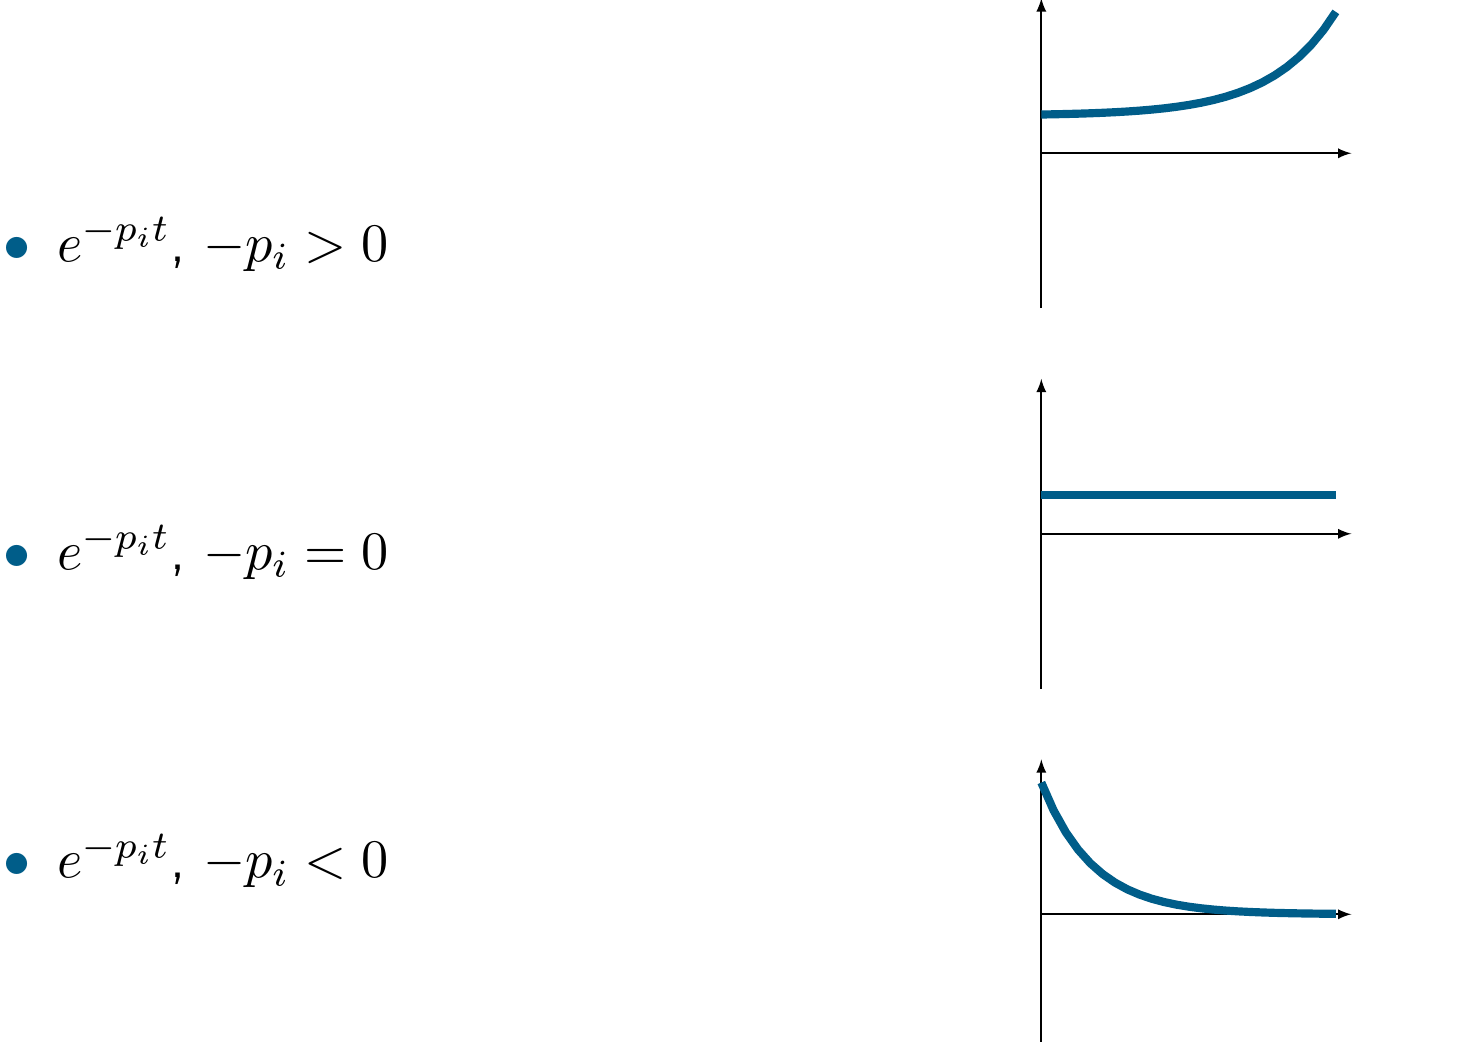
\includegraphics[scale=0.2]{Images/Modi_naturali_poli_distinti_1.png}
    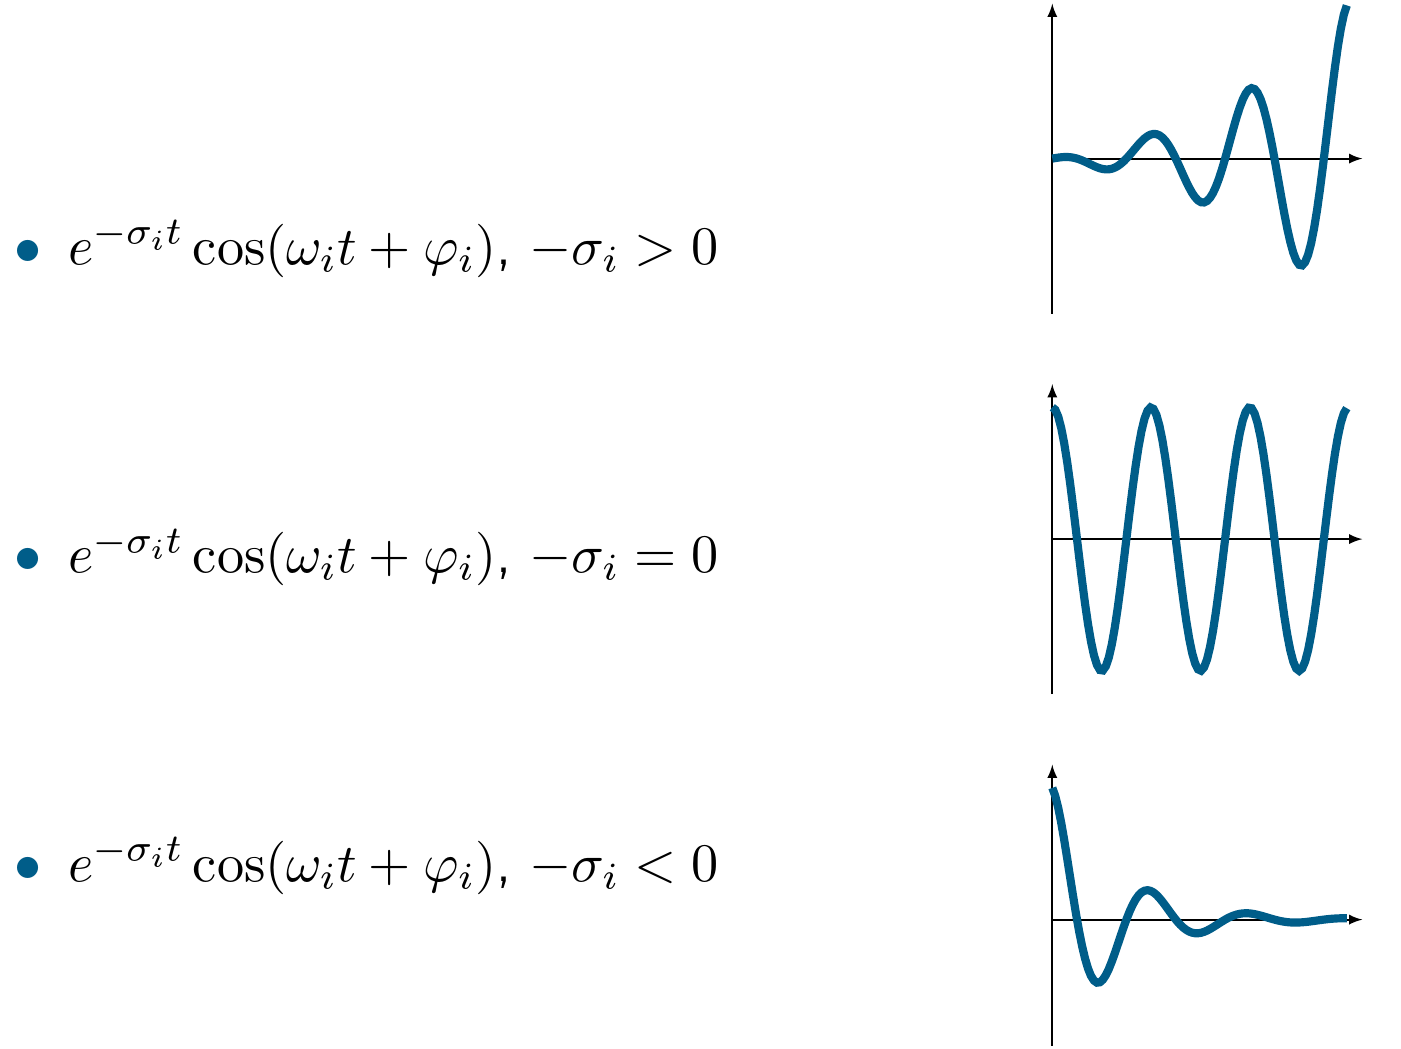
\includegraphics[scale=0.2]{Images/Modi_naturali_poli_distinti_2.png}
    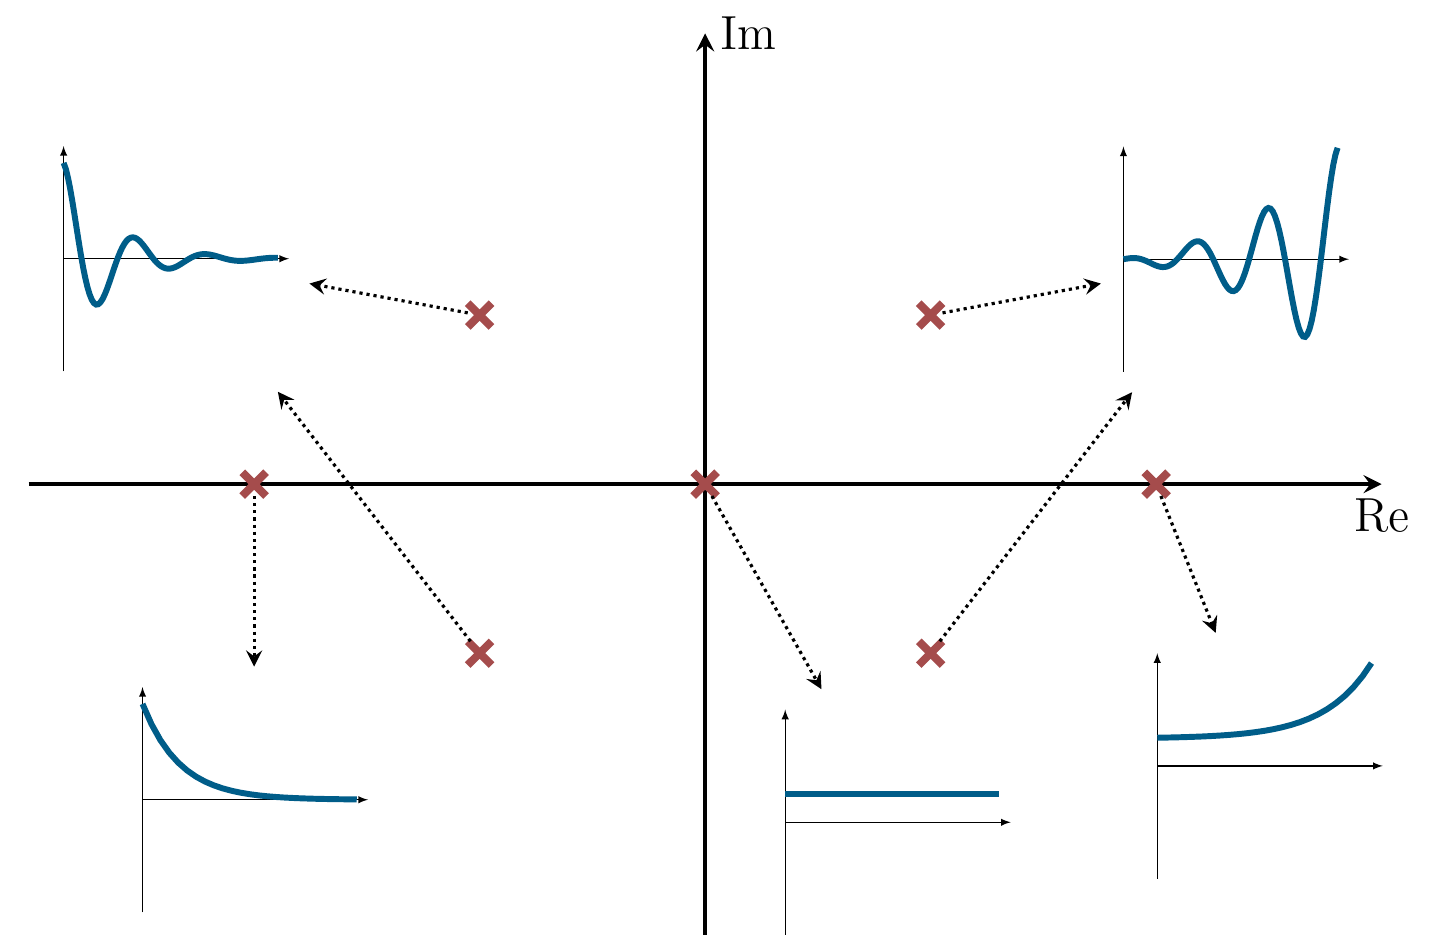
\includegraphics[scale=0.2]{Images/Modi_naturali_poli_distinti_3.png}
\end{center}


\subsection{Caso 2: Poli reali o complessi coniugati multipli con molteplicità maggiore di 1}
\begin{equation}
    Y(s) = \frac{N(s)}{D(s)} = \frac{N(s)}{\prod\limits_{i=1}^q (s + p_i)^{n_i}} = \sum_{i=1}^q \sum_{h=1}^{n_i} \frac{k_{i,h}}{(s+p_i)^h}
\end{equation}
con $k_{i,h}, h=1,\dots, n_i$ residui del poli $-p_i$. Consideriamo
\begin{align*}
    (s+p_i)^{n_i} \frac{N(s)}{D(s)}
    &=(s+p_i)^{n_i} \sum_{\substack{j=1\\ j \neq i}}^q \sum_{h=1}^{n_j} \frac{k_{j,h}}{(s+p_j)^h} + \sum_{h=1}^{n_i} (s+p_i)^{n_i - h}k_{i,h}
    \\
    &=(s+p_i)^{n_i} \sum_{\substack{j=1\\ j \neq i}}^q \sum_{h=1}^{n_j} \frac{k_{j,h}}{(s+p_j)^h} + \sum_{h=1}^{n_i-1} (s+p_i)^{n_i - h}k_{i,h} + k_{i,n_i}
\end{align*}
Quindi il residuo $k_{i,n_i}$ è dato da
\begin{equation}
    k_{i,n_i} = (s+p_i)^{n_i} \frac{N(s)}{D(s)} \bigg|_{s=-p_i}
\end{equation}
Derivando $(s+p_i)^{n_i} \dfrac{N(s)}{D(s)}$ si calcolano gli altri residui come
\begin{equation}
    k_{i,h} = \frac{1}{(n_i-h)!} \frac{d^{n_i-h}}{ds^{n_i-h}} \left[(s+p_i)^{n_i} \frac{N(s)}{D(s)}\right] \bigg|_{s=-p_i}
\end{equation}
Antitrasformando $Y(s)$ sviluppata in fratti semplici, ricordando la \nameref{Tabella delle trasformate} e la  proprietà di \nameref{Derivazione nel dominio della variabile complessa}
\begin{align*}
    y(t) = \mathcal{L}^{-1} [Y(s)]
    &= \sum_{i=1}^q \sum_{h=1}^{n_i} k_{i,h} \mathcal{L}^{-1} \left[\frac{1}{(s+p_i)^h}\right]
    \\
    &= \sum_{i=1}^q \sum_{h=1}^{n_i} k_{i,h} \frac{t^{h-1}}{(h-1)!}e^{-p_i t}1(t)
\end{align*}



\subsubsection{Esempio}
Consideriamo la seguente trasformata di Laplace dell'uscita di un generico sistema
\[
    Y(s) = \frac{s+3}{(s+1)^2(s+2)} = \frac{k_{1,1}}{(s+1)} + \frac{k_{1,2}}{(s+1)^2} + \frac{k_{2}}{(s+2)}   
\]
\begin{align*}
    k_2 &= (s+2)Y(s) \big|_{s=-2} & k_{1,2} = (s+1)^2 Y(s) \big|_{s=-1}
\end{align*}
\begin{align*}
    k_2 
    &= \cancel{(s+2)} \frac{(s+3)}{(s+1)^2\cancel{(s+2)}} \bigg|_{s=-2}
    &
    k_{1,1}
    &= \cancel{(s+2)^2} \frac{(s+3)}{\cancel{(s+1)^2}(s+2)} \bigg|_{s=--1}
    \\
    &= \frac{(-2+3)}{(-2+1)^2}
    &
    &= \frac{(-1+3)}{(-1+2)}
    \\
    &=1
    &
    &=2
\end{align*}
\begin{align*}
    \frac{d}{ds}\left((s+1)^2 Y(s)\right)\bigg|_{s=-1} 
    &= \frac{d}{ds} \left[ \frac{k_{1,1}(s+1)^2}{(s+1)} + \frac{k_{1,2}\cancel{(s+1)^2}}{\cancel{(s+1)^2}} + \frac{k_2(s+1)^2}{s+2}\right]_{s=-1}
    \\
    &= \left[k_{1,1} + 0 + k_2 \frac{\overbrace{(s+1)^2}^{0}-2\overbrace{(s+1)}^{0}(s+2)}{(s+2)}\right]_{s=-1}
    \\
    &= k_{1,1}
\end{align*}
\begin{align*}
    k_{1,1} 
    &= \frac{d}{ds} \cancel{(s+1)^2} \frac{s+3}{\cancel{(s+1)^2}(s+2)} \bigg|_{s=-1}
    \\
    &= \frac{d}{ds}\frac{s+3}{(s+2)} \bigg|_{s=-1}
    \\
    &= \frac{(s+3)-(s+2)}{(s+2)^2}\bigg|_{s=-1}
    \\
    &= 1
\end{align*}
quindi possiamo scrivere la $Y(s)$ come
\[
    Y(s) = \frac{k_{1,1}}{(s+1)} + \frac{k_{1,2}}{(s+1)^2} + \frac{k_{2}}{(s+2)} = \frac{1}{s+1} + \frac{2}{(s+1)^2} + \frac{1}{(s+2)}
\]
ricordando la \nameref{Tabella delle trasformate} e la proprietà di \nameref{Traslazione nel dominio della variabile complessa} antitrasformiamo tutte le componenti della funzione di trasferimento
\begin{align*}
    \mathcal{L}^{-1}\left[\frac{1}{(s+2)^2}\right] &= e^{-2t} t 1(t) & \mathcal{L}^{-1}\left[\frac{1}{(s+1)^2}\right] &= e^{-t} t 1(t)
\end{align*}
\begin{align*}
    y(t) 
    &= k_{1,1}e^{-t}1(t) + k_{1,2} t e^{-t}1(t) + k_{2}e^{-2t}1(t)
    \\
    &= e^{-t}1(t) + 2 t e^{-t}1(t) +e^{-2t}1(t)
\end{align*}



\subsubsection{Forma reale per poli complessi coniugati con molteplicità maggiore di 1}
Si può dimostrare che per una coppia di poli complessi coniugati
\begin{align*}
    \sigma_i &+ j \omega_i  & \sigma_i &- j \omega_i 
\end{align*}
con molteplicità $n_i$, il contributo elementare associato è dato da
\begin{equation}
    \sum_{h=1}^{n_i} 2M_{i,h} \frac{t^{h-1}}{(h-1)!} e^{-\sigma_i t} \cos(\omega_i t + \sigma_{i,h}) 1(t)
\end{equation}
Ad esempio, consideriamo la seguente funzione di trasferimento
\[
    Y(s) = \frac{N(s)}{(s^2+2 \xi \omega_ns + \omega_n^2)}    
\]
i poli della funzione sono
\begin{align*}
    &\underbrace{-\xi \omega_n}_{\sigma} + \underbrace{j \omega_n \sqrt{1-\xi^2}}_{\omega} & -\xi \omega_n - j \omega_n \sqrt{1-\xi^2}
\end{align*}
quindi
\[
    Y(s) = \frac{N(s)}{(s + \sigma + j \omega) (s + \sigma - j \omega)}
\]
\begin{align*}
    &2M_{1,1}e^{-\sigma t}\cos(\omega t+\varphi)1(t) + 2M_{1,2}t e^{-\sigma t} \cos(\omega t + \varphi)1(t)\\ =& 2M_{1,1}e^{-\xi \omega_n t} \cos(\omega_n \sqrt{1 - \xi^2}t+\varphi)1(t) + 2M_{1,2}e^{-\xi \omega_n t} \cos(\omega_n \sqrt{1 - \xi^2}t+\varphi)1(t)
\end{align*}


\subsubsection{Modi naturali di poli multipli}
Un modo naturale di un polo reale multiplo $-p_i$ è definito come
\begin{equation}
    \frac{t^{h-1}}{(h-1)!} e^{-p_i t} 1(t)
\end{equation}
I modi naturali di una coppia di poli complessi coniugati multipli $-(\sigma_i + j \omega_i)$ e $-(\sigma_i - j \omega_i)$ sono definiti come
\begin{equation}
    \frac{t^{h-1}}{(h-1)!} e^{-\sigma_i t} \cos(\omega_i + \varphi_{i,h}) 1(t)
\end{equation}
\begin{center}
    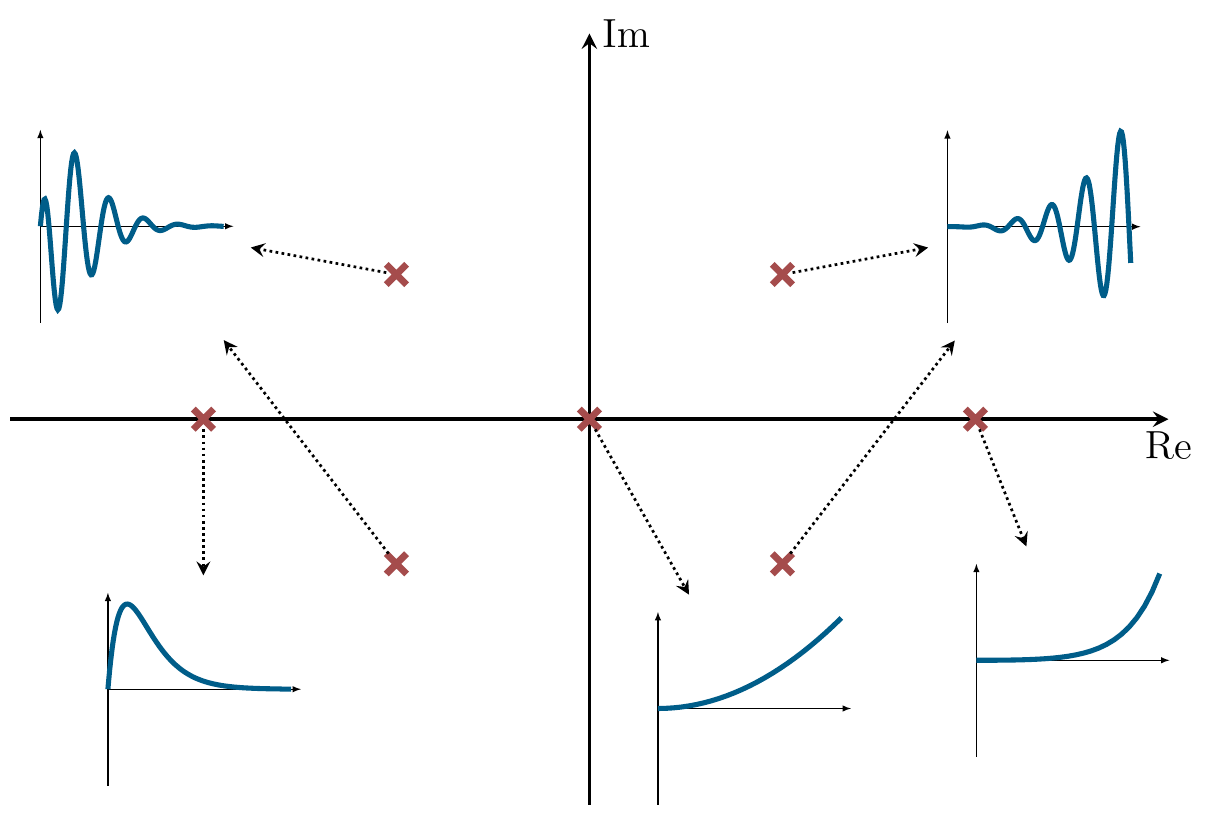
\includegraphics[scale=0.2]{Images/Modi_naturali_poli_multipli.png}
\end{center}


\subsubsection{Modi naturali come risposta all'impulso}
Sappiamo che per $x(0)=0$ (risposta forzata)
\[
    Y(s) = G(s) U(s)
\]  
se applichiamo in ingresso una delta di Dirac $u(t)=\delta(t)$
\[
    Y(s) = G(s)    
\]
Quindi la risposta ad un impulso è una combinazione lineare dei modi naturali del sistema lineare tempo invariante (SISO) descritto da $G(s)$.



\subsection{Risposta a un ingresso generico}
Ricordiamo che 
\[
    Y(s) = \underbrace{C(sI-A)^{-1}}_{\begin{array}{c}\frac{N_\ell(s)}{D(s)}\end{array}} -x(0) + \underbrace{G(s)U(s)}_{\begin{array}{c}\frac{N_f(s)}{D(s)}\frac{N_u(s)}{D_u(s)}\end{array}}
\]
in cui $C(sI-A)^{-1} x(0)$, $G(s)$ e $U(s)$ sono rapporti di polinomi.\\
Quindi
\begin{align*}
    y(t) 
    &= y_\ell(t) + y_f(t)
    \\
    &=y_\ell(t) + y_{f,G}(t) + y_{g,U}(t)
\end{align*}
in cui 
\begin{itemize}
    \item  $y_\ell (t)$ e $y_{f,G} (t)$ sono combinazioni lineari di modi naturali del sistema con matrici $A, B, C$ e $D$;
    \item $y_{f,U} (t)$ è combinazione lineare di "modi" presenti nell'ingresso $u(t)$ (dovuti alle radici del denominatore di $U (s)$).
\end{itemize}



\subsection{Risposta di sistemi elementari}
Ricordiamo la \ref{parametrizzazione 1} 
\[
    G(s) = \frac{\rho \prod_i (s + z_i)\prod_i (s^2+2 \zeta_i \alpha_{ni}s  +\alpha^2_{ni})}
                {s^g \prod_i (s + p_i)\prod_i (s^2+2 \xi_i \omega_{ni}s + \omega^2_{ni})}
\]
Consideriamo il caso di poli distinti. Da quanto visto fino ad ora risulta che per $x(0) = 0$ (risposta forzata)
\[
    Y(s) = G(s)U(s) = \sum_{i} \frac{k_i}{s+p_i} + \sum_i \frac{a_i s+b_i}{s^2 + 2\xi_i\omega_{n,i}s + \omega^2_{n,i}}
\]
\begin{center}
    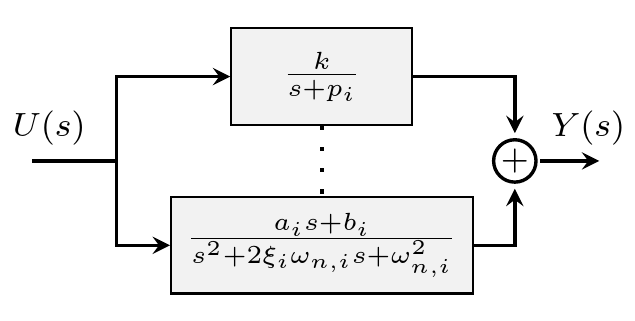
\includegraphics[scale=0.27]{Images/Risposta_sistemi_elementari.png}
\end{center}


\subsection{Stabilità esterna (BIBO)}
Un sistema si dice BIBO (Bounded-Input Bounded-Output) stabile se la sua uscita forzata è limitata per ogni ingresso limitato.
\vspace*{0.1cm}\\
Da quanto visto fino ad ora con lo sviluppo di Heaviside (fratti semplici) si può dedurre che un sistema con funzione di trasferimento $G(s)$ è BIBO stabile se e solo se tutti i poli di $G(s)$ sono a parte reale strettamente minore di zero.
\vspace*{0.1cm}\\
\textbf{N.B.} La BIBO stabilità è equivalente alla stabilità asintotica. 



\section{Analisi di sistemi attraverso funzione di trasferimento}
%in riferimento al pacchetto di slide "main_CAT_modulo2_part4"


\subsection{Dalla Funzione di Trasferimento allo spazio degli stati}
Consideriamo la funzione di trasferimento
\[
    G(s) = \frac{\mu}{1+T s}
\]  
Questo tipo di sistemi può essere rappresentato nello spazio degli stati (la rappresentazione non è unica) come
\begin{align}\label{sis_1_ordine}
    \dot x &= - \frac{1}{T} x + \frac{\mu}{T}\mu
    \\
    y = x
\end{align}
Infatti, la funzione di trasferimento associata a \ref{sis_1_ordine} è 
\[
    G(s) = C(sI-A)^{-1} B = \frac{\mu}{1+Ts}
\]
dove 
\begin{itemize}
    \item il parametro $T$ è la costante di tempo associata al polo;
    \item il parametro $\mu$ è il \textit{guadagno}
\end{itemize}


\subsection{Sistemi del primo ordine}
Definiamo un sistema nello spazio della funzione di trasferimento
\begin{align*}
    G(s) &= \frac{\mu}{1+T s} & U(s) = \frac{k}{s}\\
\end{align*}
\[
    Y(s) = G(s) U(s) = \frac{\mu k}{s(1+T s)}
\]
con $\mu >0,k>0,T>0$; da notare che se $T<0$ il sistema è instabile perché si avrebbe un polo positivo.
\vspace*{0.1cm}\\
Allora mediante lo sviluppo di Heaviside e la formula di antitrasformazione troviamo che
\[
    y(t) = \mu k(1-e^{-t/T})1(t)
\]
$y(0) = 0, \dot y(0) = \dfrac{\mu k}{T} , y_{\infty} = \mu k$
\begin{center}
    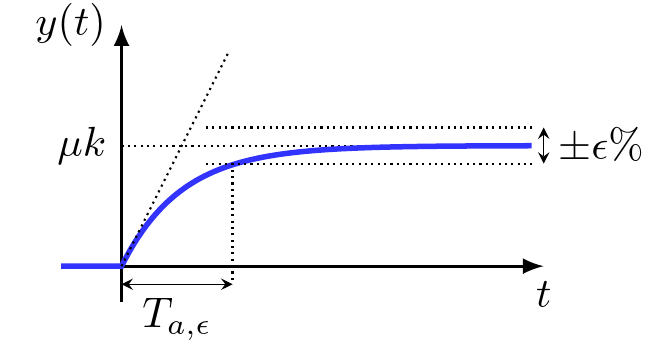
\includegraphics[scale=0.27]{Images/Sistemi_1_ordine_1.png}
\end{center}
Definiamo il \textbf{tempo di assestamento} $\mathbf{T_{\alpha,\epsilon}}$ come il tempo tale per cui $(1-0.001\epsilon)y_{\infty} \leq y(t) \leq (1+0.01\epsilon)y_{\infty} \ \forall t \geq T_{\alpha,\epsilon}$.

\subsubsection{Esempio}
Consideriamo un sistema con 
\begin{align*}
    G(s) = \frac{\mu}{1+T s} = \frac{\mu}{T} \frac{1}{s+\frac{1}{T}}
\end{align*}
con ingresso $u(t)=k 1(t)$, quindi $U(s) = \frac{k}{s}$
\begin{align*}
    Y(s) 
    &= G(s) U(s)
    \\
    &=  \frac{\mu}{T} \frac{1}{s+\frac{1}{T}} \frac{k}{s}
    \\
    &= \frac{k_1}{s+\frac{1}{T}} + \frac{k_2}{s}
\end{align*}
\begin{align*}
    y(t)
    &= \mathcal{L}^{-1} \underbrace{\left[\frac{k_1}{s+\frac{1}{T}}\right]}_{y_{G,t}} + \mathcal{L}^{-1} \underbrace{\left[\frac{k_2}{s}\right]}_{y_{U,t}}
    \\
    &= k_1 \underbrace{e^{-t/T}}_{\T{sistema}} + k_2 \underbrace{1(t)}_{\T{ingresso}}
\end{align*}
\begin{align*}
    k_1 
    &= (s+\frac{1}{T})Y(s) \big|_{s=-1/T}
    &
    k_2
    &= sY(s) \big|_{s=0}
    \\
    &= \cancel{\left(s+\frac{1}{T}\right)}\frac{\mu}{T}\frac{k}{\left(\cancel{s+\frac{1}{T}}\right)s}\bigg|_{s=-1/T}&
    &=\frac{\mu}{T} \frac{k}{s+\frac{1}{T}} \bigg|_{s=0}
    \\
    &=\frac{\mu}{T} \frac{k}{-\frac{1}{T}}&
    &= \mu k
    \\
    &= -\mu k
\end{align*}
\begin{align*}
    y(t)
    &= - \mu k e^{-t/T}1(t) + \mu k 1(t)
    \\
    &= \mu k (1 - e^{-t/T}) 1(t)
\end{align*}
La risposta ottenuta ci dice che dando in ingresso il gradino, il sistema ci metterà un po' per raggiungerlo, in base alla sua dinamica.
\vspace*{0.1cm}\\
Per quanto riguarda invece il tempo di assestamento, esso si calcola
\[
    T_{\alpha,\epsilon} = T \ln \left(\frac{1}{0.01\epsilon}\right)    
\]
\begin{align*}
    T_{\alpha,5} &\approx 3T & T_{\alpha,1} &\approx 4.6T
\end{align*}


\subsubsection{Considerazioni}
\begin{itemize}
    \item Per calcolare la risposta riscrivere $G(s) = \dfrac{\mu}{T} \dfrac{1}{s+\frac{1}{T}}$ e sviluppare $Y (s) = G(s)U (s)$ in fratti semplici;
   \item la risposta è monotona, i modi presenti sono $1(t)$ dell' ingresso e $e^{-t/T}$ del sistema;
   \item il valore asintotico è $\mu k$, quindi se l'ingresso fosse un riferimento $k$ da seguire, avremmo un errore a regime $e_{\infty} = |1-\mu|k$.
\end{itemize}




\subsection{Sistemi del secondo ordine}
La funzione di trasferimento di sistemi del secondo ordine è 
\begin{equation}
    G(s) = \mu\frac{\omega^2_n}{s^2+2 \xi \omega_n + \omega^2_n}
\end{equation}
Questo tipo di sistemi può essere rappresentato nello spazio degli stati come
\begin{align*}
    \dot x_1 &= x_2\\
    \dot x_2 &= - \omega^2_n - 2 \xi \omega_nx_2 + \mu \omega^2_n u\\
    y &= x_1
\end{align*}
dove
\begin{itemize}
    \item il parametro $\xi$ è il coefficiente di smorzamento;
    \item il paramento $\omega_n$ è la pulsazione naturale;
    \item il parametro $\mu$ è il guadagno.
\end{itemize}


\subsubsection{Sistemi del secondo ordine con poli complessi coniugati}
\begin{align*}
    G(s) &= \mu\frac{\omega^2_n}{s^2+2 \xi \omega_n + \omega^2_n} & U(s) &= \frac{k}{s}
    \\
    Y(s) &= G(s)U(s) = \mu k \frac{\omega^2_n}{s(s^2+2 \xi \omega_n + \omega^2_n)}
\end{align*}
con $|\xi|<1$ e $\omega_n > 0$
\[
    y(t) = \mu k(1 - Ae^{-\xi \omega_n t}\sin(\omega t + \varphi))1(t)
\]
\begin{align*}
    A &= \frac{1}{\sqrt{1-\xi^2}} & \omega &= \omega_n\sqrt{1 - \xi^2} & \varphi &= \arccos(\xi)
\end{align*}
\begin{align*}
    y(0) &= \dot y(0) = 0 & \ddot y(0) &= \mu \omega^2_n & y_{\infty} &= \mu k
\end{align*}
\begin{align*}
    T_{a,5} &\approx \frac{3}{\xi \omega_n} & T_{a,1} \approx \frac{4.6}{\xi \omega_n}
\end{align*}
Introduciamo un altro parametro che è la \textbf{sovraelongazione percentuale}, definita come
\begin{equation}
    S\% = 100 \frac{y_{\T{max}} - y_\infty}{y_{\infty}}
\end{equation}
con $y_{\T{max}}$ valore massimo e $y_{\infty}$ valore asintotico della risposta.
\vspace*{0.1cm}\\
Per i sistemi del secondo ordine la sovraelongazione percentuale vale
\begin{equation}
    S\% = 100 e^{-\pi \xi / \sqrt{1-\xi^2}}
\end{equation}
\vspace*{0.2cm}
Analizziamo ora la risposta
\[
    y(t) = \mu k(1 - Ae^{-\xi \omega_n t}\sin(\omega t + \varphi))1(t)
\]
\begin{center}
    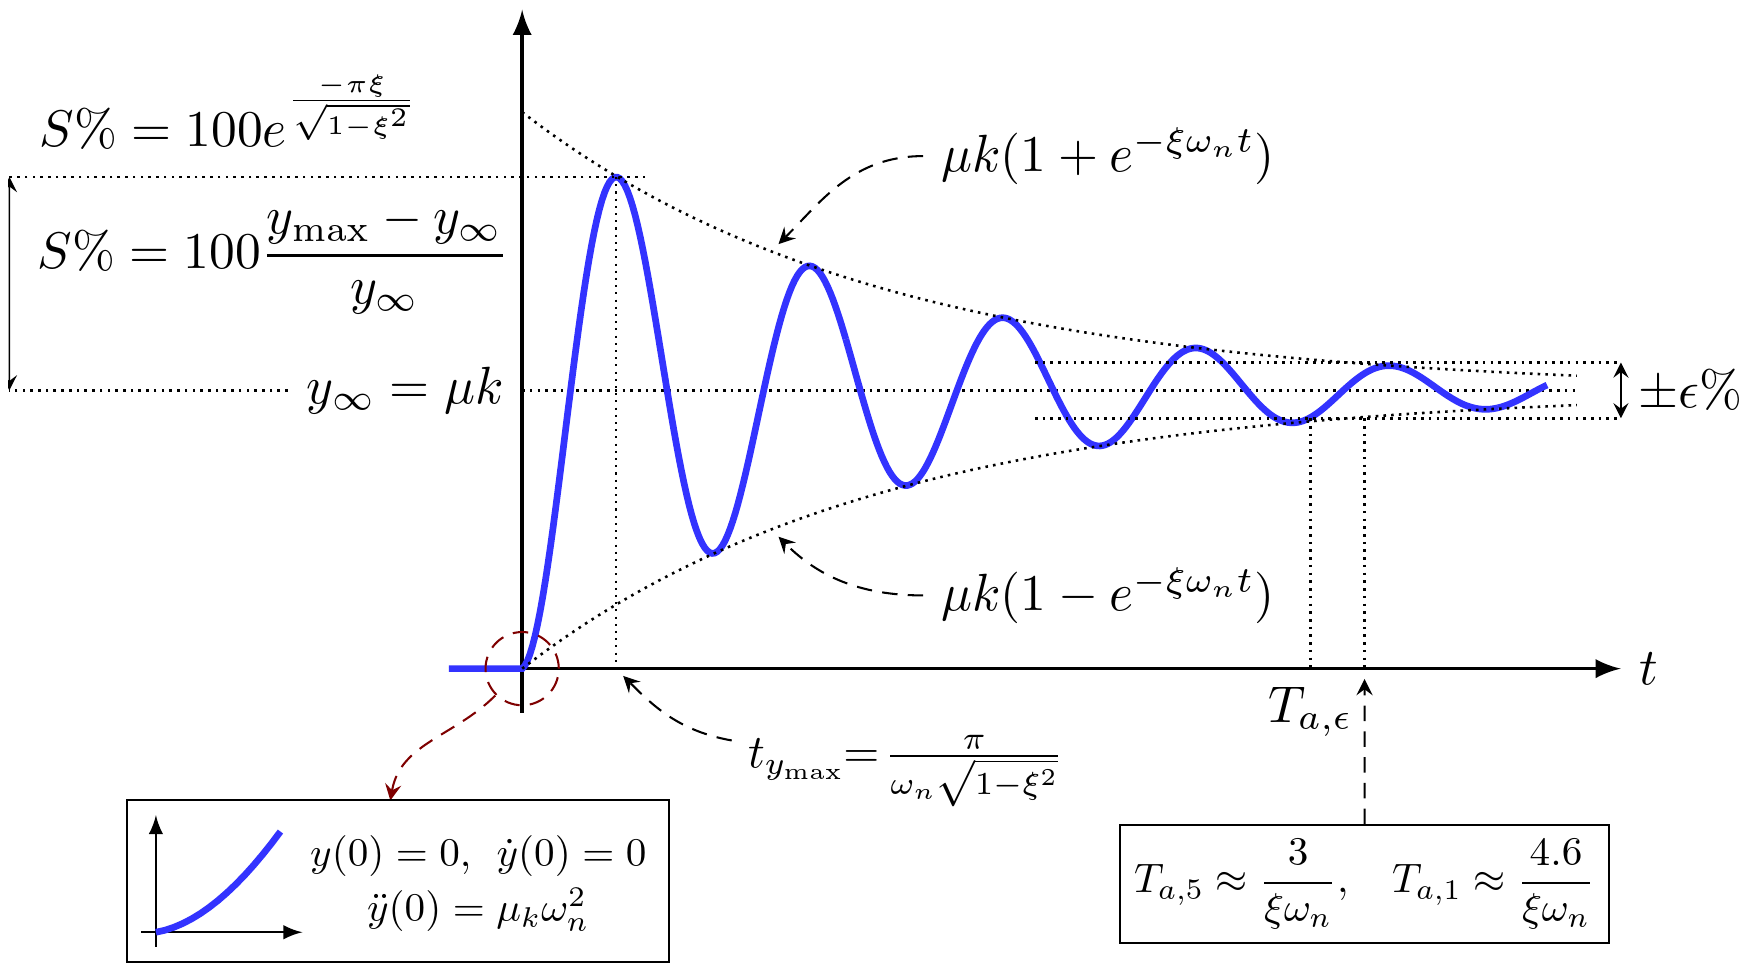
\includegraphics[scale=0.23]{Images/Sovraelongazione.png}
\end{center}
Dal grafico possiamo evincere che la sovraelongazione percentuale indica di quanto supero il valore stabile prima del transitorio.\\
Come abbiamo visto prima, la sovraelongazione percentuale dipende solo dallo smorzamento, e, se scegliamo un valore massimo di sovraelongazione $S^*$, possiamo ricavare il valore di $\xi$ necessario:
\begin{align*}
    S\% \leq S^* \Longleftrightarrow \xi \geq \frac{\Bigg| \ln \left(\dfrac{S^*}{100}\right) \Bigg|}{\sqrt{\pi^2 + \ln^2 \left( \dfrac{s^*}{100}\right)}}
\end{align*}


\subsubsection{Luogo di punti a tempo di assestamento costante}
Adesso proviamo a caratterizzare i sistemi del secondo ordine (con poli complessi coniugati) la cui risposta al gradino ha lo stesso tempo di assestamento.
\vspace*{0.1cm}\\
Ricordiamo che 
\begin{itemize}
    \item abbiamo approssimato $T_{a,5} \approx \frac{3}{\xi \omega_n}$ e $T_{a,1} \approx \frac{4.6}{\xi \omega_n}$
    \item $-\xi \omega^n$ è la parte reale dei poli complessi coniugati
\end{itemize}
\begin{center}
    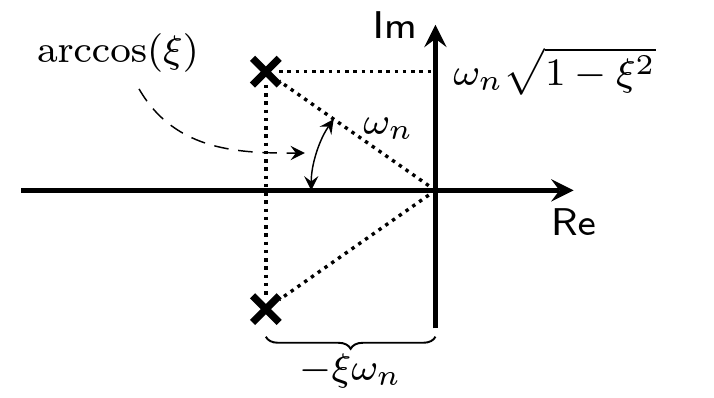
\includegraphics[scale=0.23]{Images/Secondo_ordine_poli_complessi.png}
\end{center}
Quindi sistemi con poli complessi coniugati che hanno la stessa parte reale avranno una risposta al gradino con stesso tempo di assestamento.
\vspace*{0.2cm}\\
Sul piano complesso i luoghi di punti a tempo di assestamento costante sono rette parallele all'asse immaginario.
\begin{center}
    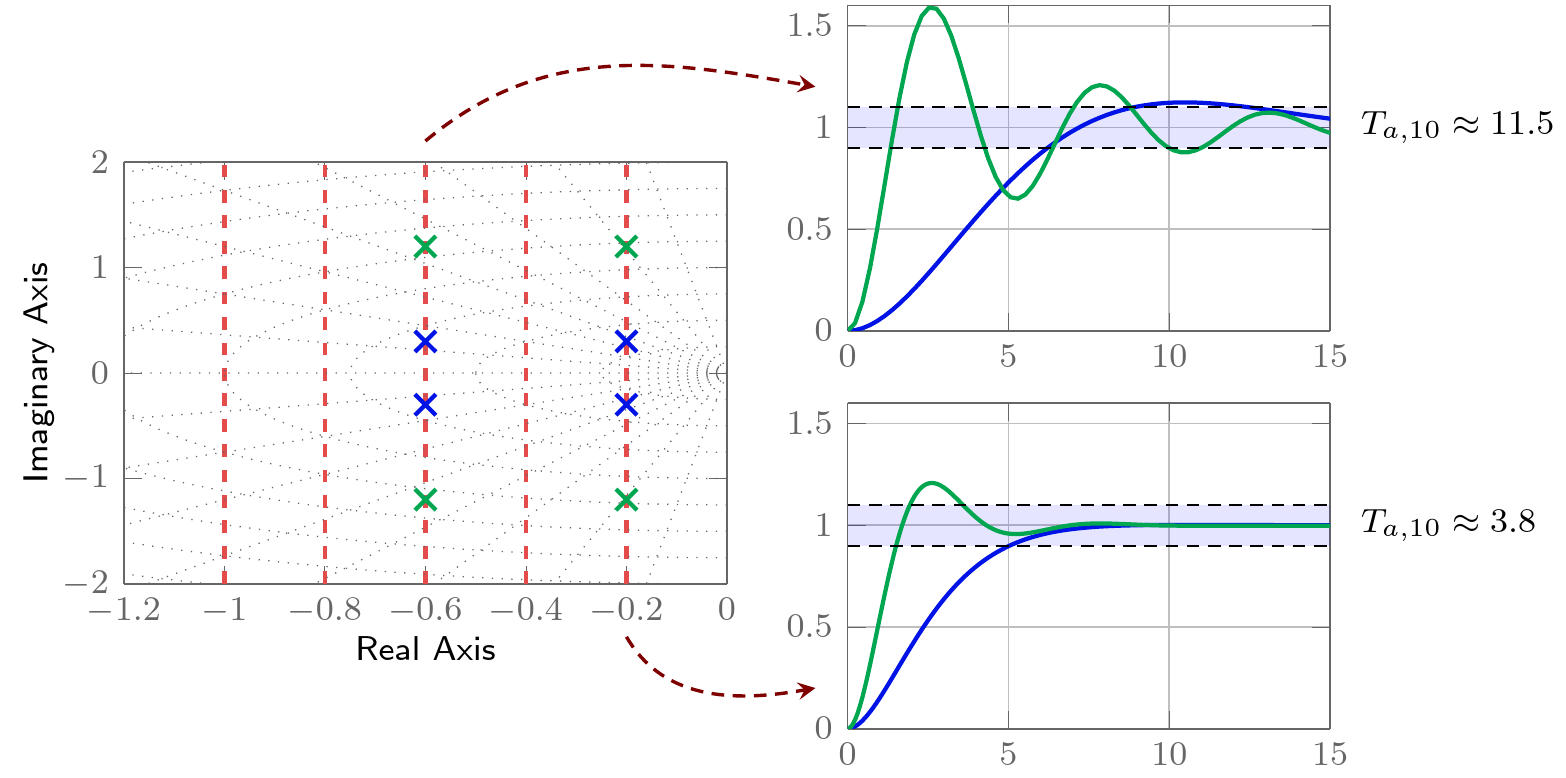
\includegraphics[scale=0.23]{Images/Tempo_assestamento_costante.png}
\end{center}
Nella figura vediamo in verde e in blue due coppie di poli distinti, ma con parte reale uguale; le risposte associate a questi poli sono evidentemente diverse (grafico in blue e grafico in verde), ma hanno lo stesso tempo di assestamento.


\subsubsection{Luogo di punti a sovraelongazione costante}
Proviamo a caratterizzare e i sistemi del secondo ordine (con poli complessi coniugati) la cui risposta al gradino ha la stessa sovraelongazione.
\vspace*{0.1cm}\\
Ricordiamo che 
\begin{itemize}
    \item $S\% = 100 e^{\frac{-\pi \xi}{\sqrt{1-\xi^2}}}$
    \item $\arccos(\xi)$ è l'angolo formato con l'asse reale
\end{itemize}
\begin{center}
    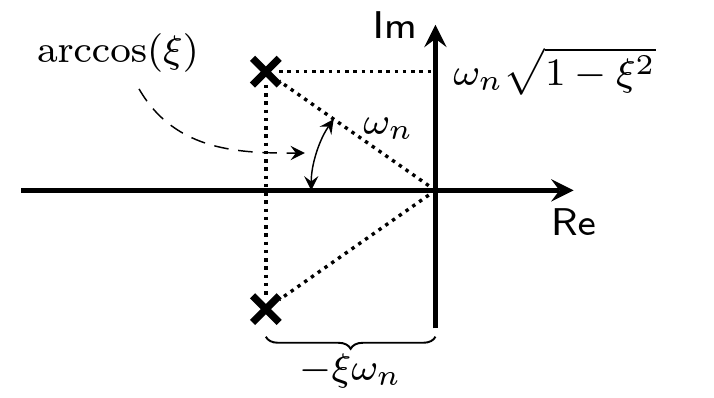
\includegraphics[scale=0.23]{Images/Secondo_ordine_poli_complessi.png}
\end{center}
Quindi sistemi con stesso coefficiente di smorzamento $\xi$ avranno una risposta al gradino con stessa sovraelongazione.
\vspace*{0.1cm}\\
Sul piano complesso i luoghi di punti a sovraelongazione costante sono semirette uscenti dall'origine.
\begin{center}
    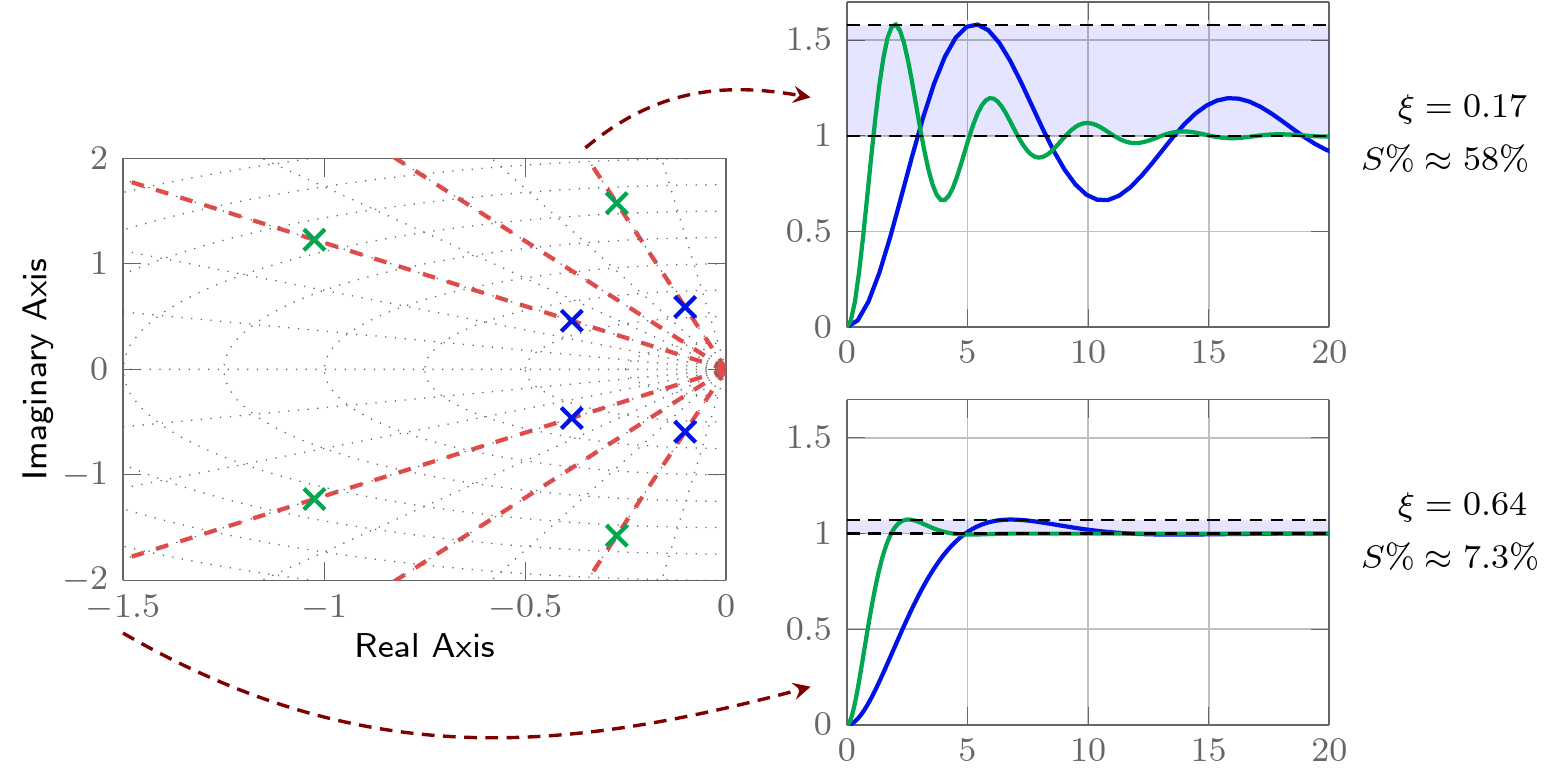
\includegraphics[scale=0.23]{Images/Sovraelongazione_costante.png}
\end{center}


\subsubsection{Mappatura di specifiche temporali nel piano complesso}
Vogliamo caratterizzare i sistemi del secondo ordine (con poli complessi coniugati) con $S\% \leq S^*$ e $T_{a,5} \leq T^*$. 
\vspace*{0.1cm}\\
Le specifiche sono soddisfatte per $\xi \geq \xi^*$ (con $\xi \leq 1$) e $\xi \omega_n \geq \dfrac{3}{T^*}$ 
\begin{center}
    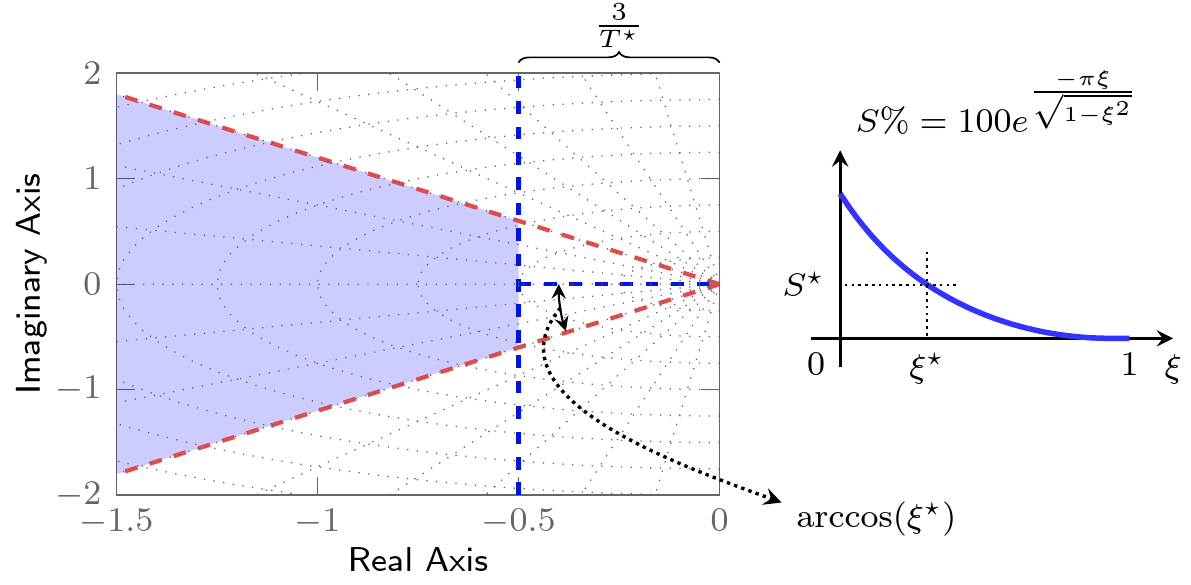
\includegraphics[scale=0.23]{Images/Specifiche_temporali.png}
\end{center}
i poli complessi coniugati devono trovarsi nella zona colorata.


\subsubsection{Sistemi del secondo ordine con poli reali}
Caso $T_1 \neq T_2$ e $T_1 > T_2$
\begin{align*}
    G(s) &= \frac{\mu}{(1+T_1s)(1+T_2s)} & U(s) &= \frac{k}{s}\\
    Y(s) &= G(s)U(s) = \frac{\mu k}{s(1+T_1s)(1+T_2s)} 
\end{align*}
\begin{align*}
    &\mu>0 & &k>0 & &T_1>0 & &T_2>0
\end{align*}
\begin{center}
    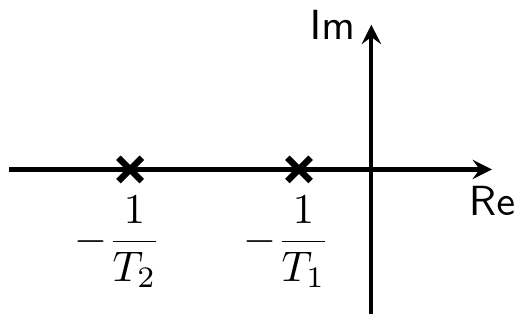
\includegraphics[scale=0.23]{Images/Secondo_ordine_poli_reali_1.png}
\end{center}
\[
    y(t) = \mu k \left(1- \frac{T_1}{T_1-T_2}e^{-\frac{t}{T_1}} + \frac{T_2}{T_1-T_2}e^{-\frac{t}{T_2}}\right)1(t)
\]
\begin{align*}
    &y(0) = 0 & &\dot y(0)=0 & &\ddot y(0) = \frac{\mu K}{T_1 T_2} & &y_{\infty}=\mu k
\end{align*}
\begin{center}
    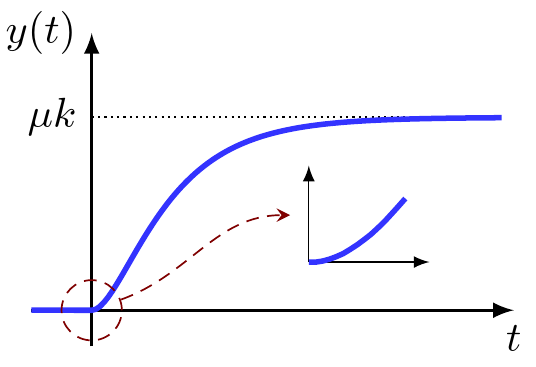
\includegraphics[scale=0.27]{Images/Secondo_ordine_poli_reali_2.png}
\end{center}


\subsection{Sistemi a polo dominante}
Consideriamo $T_1\gg T_2$:
\begin{center}
    \begin{tikzpicture}
            \begin{axis}[
                xmin=0,xmax=20,
                ymin=0,ymax=2,
                ticks=none, %elimina i valori numerici
                axis x line=middle,
                axis y line=middle,
                xlabel={$x$},
                ylabel={$y$},
                ]
                \addplot[domain=0:20, samples=100]{exp(-(x/15))}node [pos=0.1,anchor=south west]{$e^{-\frac{t}{T_1}}$};
                \addplot[domain=0:20, samples=100]{exp(-(x/2))}node [pos=0.2,anchor=south west]{$e^{-\frac{t}{T_2}}$};
            \end{axis}
        \end{tikzpicture}
    \end{center}
Nella risposta $e^{-\frac{t}{T_2}}$ tende a zero velocemente, mentre $\dfrac{T_2}{T_1-T_2}\ll\dfrac{T_1}{T_1\ll T_2} \approx 1$, quindi
\[
    y(t) \approx \mu k\left(1-e^{-\frac{t}{T_1}}\right)1(t)
\]

\begin{center}
    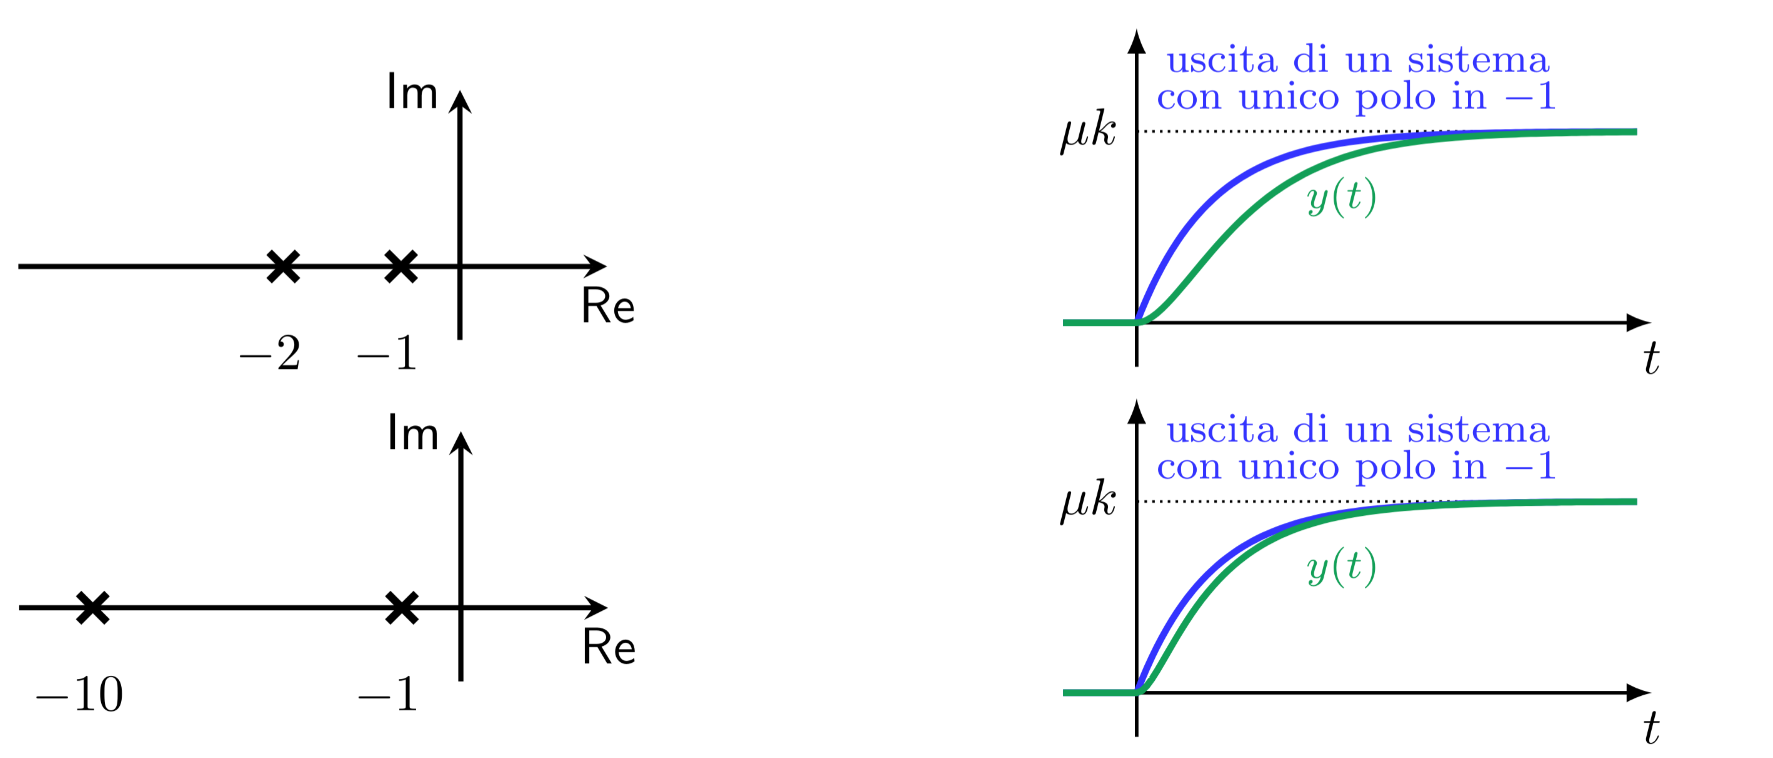
\includegraphics[scale=0.25]{Images/Polo_dominante.png}
\end{center}
\subsubsection{Esempio con coppia di poli complessi coniugati dominanti} 
\[
    G(s) = \mu \frac{\omega_n^2}{(s^2+2\xi\omega_n s +\omega_n^2)(s+p)}
\]
assumiamo $\dfrac{1}{T} \gg \xi \omega_n$, cioè $-\dfrac{1}{T} \ll - \xi \omega_n$
\begin{center}
    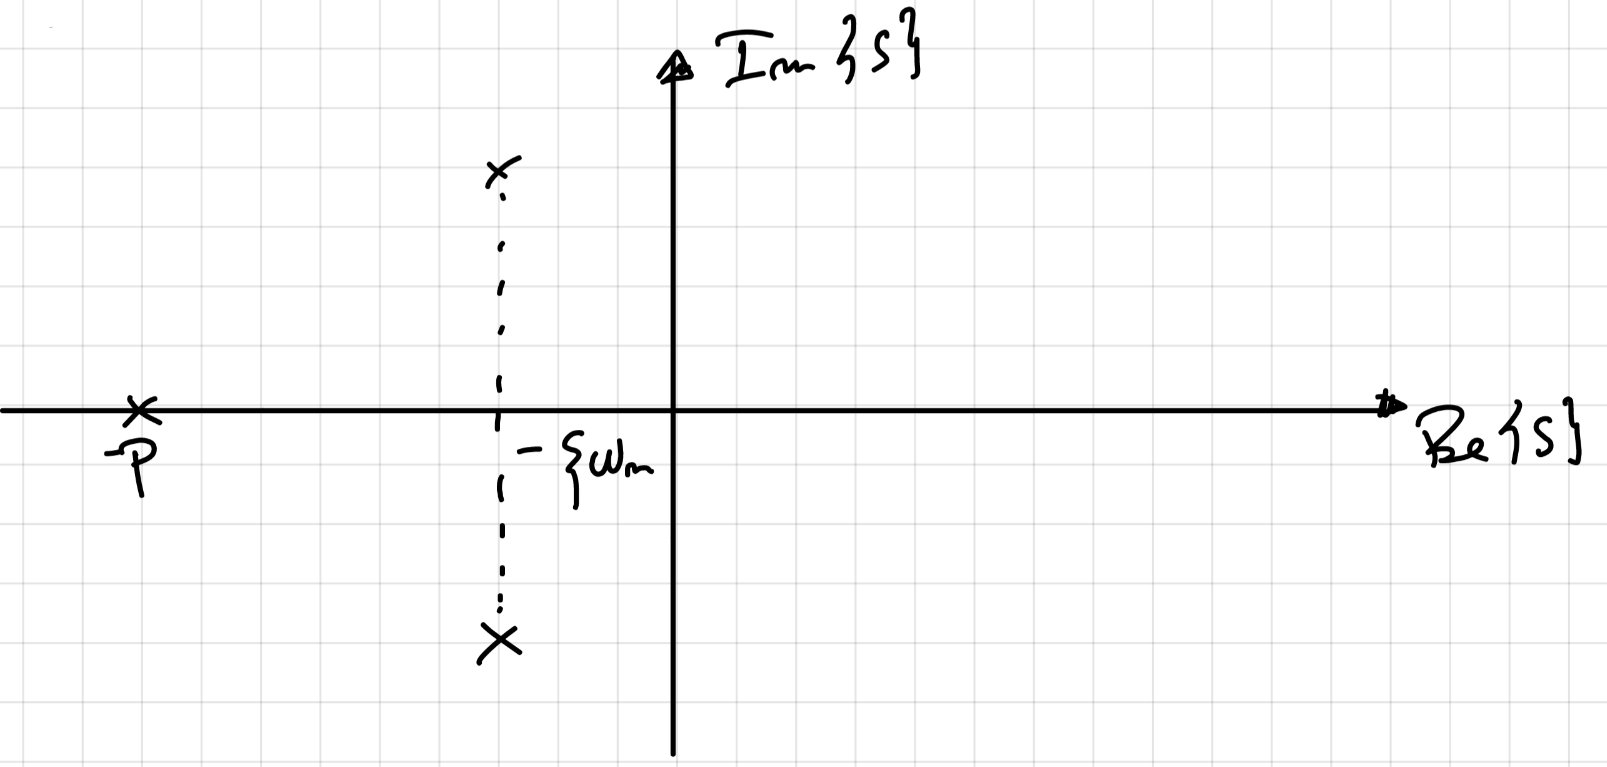
\includegraphics[scale=0.22]{Images/Esempio_polo_dominante.png}
\end{center}
Prendiamo $U(s) = \dfrac{k}{s}$
\begin{align*}
    Y(s) 
    &= G(s) U(s)\\
    &=\frac{\mu k \dfrac{\omega_n^2}{T}}{s(s^2+2\xi\omega_ns + \omega_n^2)\left(s+\dfrac{1}{T}\right)}\\
    &= \frac{k_1}{s} + \frac{k_2}{s+\xi\omega_n+j\omega_n \sqrt{1-\xi^2}} + \frac{\overline{k_2}}{s+\xi\omega_n-j\omega_n \sqrt{1-\xi^2}} + \frac{k_3}{s+\dfrac{1}{T}}
\end{align*}
Per $\dfrac{1}{T} \gg \xi \omega_n$ la risposta si può approssimare a quella di sistemi del secondo ordine
\[
    y(t) \approx \mu k \left(1-A e^{-\xi \omega_n t} \sin(\omega t + \varphi)\right)
\]
Quindi, se ho più poli molto distanti dall'asse immaginario, posso sempre approssimare il sistema come un sistema del secondo ordine.
\vspace*{0.2cm}\\
Infatti se analizziamo la risposta effettiva del sistema
\[
    y(t) = k_1 1(t) + 2M e^{-\ xi \omega_n t} \cos(\omega_n \sqrt{1 - \xi^2}t + \varphi_k) 1(t) + k_3 e^{-t/T} 1(t)
\]
il termine $k_3 e^{-t/T} 1(t)$ va a 0 molto velocemente, quindi è trascurabile.



\subsection{Sistemi del secondo ordine con poli reali coincidenti}
Caso $T_1=T_2$
\begin{align*}
    G(s) &= \frac{\mu}{(1+T_1s)^2} & U(s) &= \frac{k}{s}\\
    Y(s) &= G(s)U(s) = \frac{\mu k}{s(1+T_1 s)^2}
\end{align*}
$\mu>0, k>0, T_1 >0$
\[
    y(t) = \mu l \left( 1- e^{-t/T_1} - \frac{t}{T_1}e^{_-t/T_1} \right) 1(t)
\]
\begin{center}
    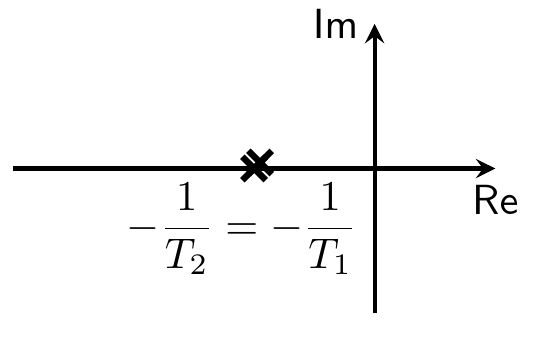
\includegraphics[scale=0.23]{Images/Poli_reali_coincidenti.png}
\end{center}
I modi presenti sono $1(t)$ (ingresso), $e^{-t/T-1}$ e $t e^{-t/T-1}$ (sistema).



\subsection{Sistemi del primo ordine con uno zero}
\begin{align*}
    G(s) &= \mu \frac{1+ \alpha T s}{1+Ts} & U(s) &= \frac{k}{s}\\
    Y(s) &= G(s) U(s) = \mu k \frac{1+ \alpha T s}{s(1+Ts)}
\end{align*}
$\mu>0, k>0, T>0$
\begin{center}
    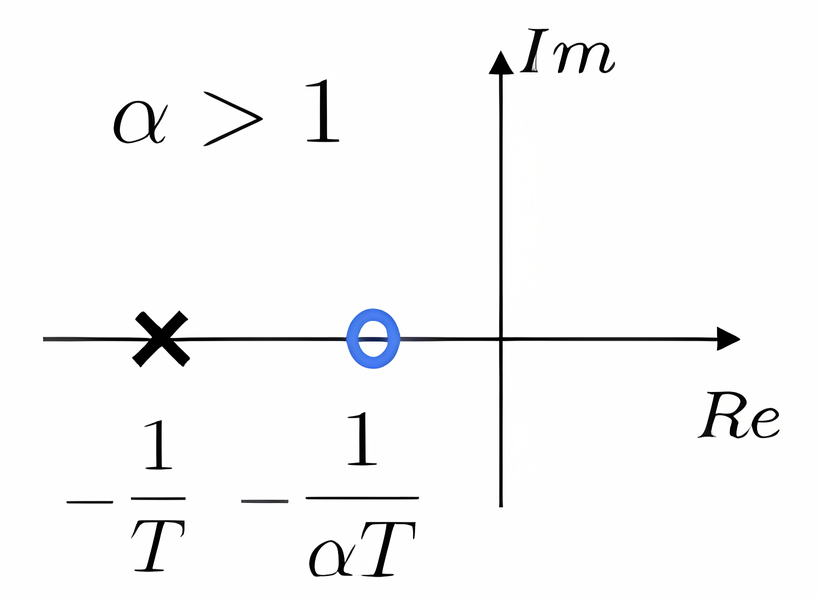
\includegraphics[scale=0.17]{Images/Primo_ordine_uno_zero_1.png}
\end{center}
\begin{align*}
    y(t) &= \mu k (1+(\alpha-1) e^{-t/T})1(t)\\
    y(0) &= \mu \alpha k & y_{\infty} &= \mu k
\end{align*}
\begin{center}
    \includegraphics[scale=0.16]{Images/Primo_ordine_uno_zero_2.png}
\end{center}
Il grado relativo del sistema è zero, cioè il grado del numeratore è uguale al grado del denominatore; questo implica un collegamento algebrico tra ingresso e uscita, infatti $y(0) \neq 0$; nello spazio degli stati questo equivale ad avere $D \neq 0$.


\subsection{Sistemi del secondo ordine con poli reali e zero}

\subsubsection{Sistemi a fase non minima}
\begin{align*}
    G(s) &= \mu\frac{1 + \tau s}{(1+T_1s)(1+T_2s)} & U(s) &= \frac{k}{s}\\
    Y(s) &= G(s)U(s) = \mu k \frac{1+ \tau s}{s(1+T_1s)(1+T_2s)}
\end{align*}
$\mu>0,k>0,T_1>0,T_2>0$
\begin{align*}
    y(t) &= \mu k \left( 1 - \frac{T_1-\tau}{T_1-T_2} e^{-t/T-1} + \frac{T_2-\tau}{T_1-T_2}e^{-t/T_2} \right)1(t)\\
    y(0) &= 0 & \dot y(0) &= \frac{\mu K \tau}{T_1T_2} & y_{\infty} &= \mu k
\end{align*}
\textbf{N.B.} il segno della derivata $\dot y(0)$ dipende da $\tau$.
\vspace*{0.2cm}\\
Nel caso in cui si abbia $T_1>T_2$ e $\tau<0$ il sistema è detto a \textbf{fase non minima}; in generale è detto sistema a \textbf{fase minima} un sistema caratterizzato da una funzione di trasferimento $G(s)$ con guadagno positivo, poli e zeri a parte reale negativa o nulla e non contenente ritardi (cioè se non ci sono esponenziali).
\begin{center}
    \includegraphics[scale=0.16]{Images/Poli_reali_zero_1.png}
    \includegraphics[scale=0.16]{Images/Poli_reali_zero_2.png}
\end{center}
la sottoelongazione $\dot y(0)<0$ indica che il sistema inizialmente risponde in senso contrario rispetto all'ingresso.
\vspace*{0.1cm}\\
Una bici, o una moto, che sterza è un sistema a fase non minima.
\vspace*{0.1cm}\\ 
Dato un guadagno specifico, esiste \underline{uno e un solo} sistema a \textbf{fase minima} che produce quel guadagno, mentre esistono infiniti sistemi a \textbf{fase non minima} che producono lo stesso. Per più informazioni: \href{https://youtu.be/jGEkmDRsq_M}{What Are Non-Minimum Phase Systems?}.

\subsubsection*{Domanda:}
Dato un sistema a fase non minima
\[
    G(s) = \mu\frac{1 + \tau s}{(1+T_1 s)(1+T_2 s)} \tag*{$\tau < 0$}
\]  
posso progettare una $R(s) = \dfrac{1}{1+ \tau s}$ tale che
\[
    R(s) G(s) = \mu \frac{1+ \tau s}{(1+T_1 s)(1+T_2 s)(1+ \tau s)}
\]  
così da eliminare lo zero positivo?\\
Ovviamente no, perché $1+ \tau s$ è un  modello della realtà, quindi, anche se matematicamente si può semplificare, nella realtà non si annullerà mai perfettamente. 


\subsubsection{Sistemi a fase minima con sovraelongazione}
Se $\tau>T_1>T_2$ abbiamo un sistema a \textbf{fase minima} con una sovraelongazione
\begin{align*}
    G(s) &= \mu\frac{1 + \tau s}{(1+T_1s)(1+T_2s)} & U(s) &= \frac{k}{s}\\
    Y(s) &= G(s)U(s) = \mu k \frac{1+ \tau s}{s(1+T_1s)(1+T_2s)}
\end{align*}
$\mu>0,k>0,T_1>0,T_2>0$

\begin{center}
    \includegraphics[scale=0.23]{Images/Fase_minima_1.png}
\end{center}

\begin{align*}
    y(t) &= \mu k \left( 1 - \frac{T_1-\tau}{T_1-T_2} e^{-t/T-1} + \frac{T_2-\tau}{T_1-T_2}e^{-t/T_2} \right)1(t)\\
    y(0) &= 0 & \dot y(0) &= \frac{\mu K \tau}{T_1T_2} & y_{\infty} &= \mu k
\end{align*}
\begin{center}
    \includegraphics[scale=0.23]{Images/Fase_minima_2.png}
\end{center}
\textbf{Nota:} è presenta una sovraelongazione tanto più accentuata quanto più lo zero è vicino all'origine (cioè al crescere di $\tau$).


\subsubsection{Sistemi a fase minima con code di assestamento}
Se  $\tau \approx T_1 \gg T_2$ abbiamo un sistema a fase minima con code di assestamento.
\begin{align*}
    G(s) &= \mu\frac{1 + \tau s}{(1+T_1s)(1+T_2s)} & U(s) &= \frac{k}{s}\\
    Y(s) &= G(s)U(s) = \mu k \frac{1+ \tau s}{s(1+T_1s)(1+T_2s)}
\end{align*}
$\mu>0,k>0,T_1>0,T_2>0$
\begin{center}
    \includegraphics[scale=0.215]{Images/Fase_minima_code_ass_1.png}
\end{center}
\begin{align*}
    y(t) &= \mu k \left( 1 - \frac{T_1-\tau}{T_1-T_2} e^{-t/T-1} + \frac{T_2-\tau}{T_1-T_2}e^{-t/T_2} \right)1(t)\\
    y(0) &= 0 & \dot y(0) &= \frac{\mu K \tau}{T_1T_2} & y_{\infty} &= \mu k
\end{align*}
\begin{center}
    \includegraphics[scale=0.2]{Images/Fase_minima_code_ass_2.png}
\end{center}
A causa della non perfetta cancellazione polo/zero ($\tau \approx T_1$) il modo "lento" $e^{-t/T_1}$ è presente e il suo transitorio si esaurisce lentamente.








\section{Risposta in frequenza}
\subsection{Risposta a un segnale di ingresso sinusoidale}
Dato un sistema lineare tempo invariante SISO con funzione di trasferimento $G(s)$ vogliamo calcolare l'uscita in corrispondenza di un ingresso sinusoidale
\begin{equation}
    u(t) = U \cos(\omega t + \varphi)
\end{equation}
la trasformata di Laplace di questo segnale è
\begin{equation}
    U(s) = U \frac{s \cos(\varphi) - \omega \sin(\varphi)}{s^2 + \omega^2}
\end{equation}
quindi
\begin{equation}\label{trasformata sinusoide}
    Y(s) = G(s) U(s) = G(s) U \frac{s \cos(\varphi) - \omega \sin(\varphi)}{s^2 + \omega^2}
\end{equation}
Consideriamo $G(s)$ con poli \textbf{distinti a parte reale negativa (BIBO stabile)}. Sviluppando in fratti semplici si ha
\begin{equation}
    Y(s) = \sum_{i=1}^n \underbrace{\frac{k_i}{s+p_i}}_{Y_1(s)} + \underbrace{\frac{k_u}{s-j \omega} + \frac{\overline{k}_u}{s+j \omega}}_{Y_2(s)}
\end{equation}
Eseguiamo lo sviluppo di Heaviside sulla \ref{trasformata sinusoide}:
\begin{align}
    Y(s) = G(s) U(s) &= G(s) U \frac{s \cos(\varphi) - \omega \sin(\varphi)}{s^2 + \omega^2}
    \\
    &=\frac{N(s)U(s \cos(\varphi) - \omega \sin(\varphi))}{(s+p_1)(s+p_2) \dots (s+p_n)(s^2 + \omega^2)}
    \\
    &= \frac{k_1}{s+p_1} + \frac{k_2}{s+p_2} + \dots + \frac{k_n}{s+p_n} + \frac{k_u}{s-j \omega} + \frac{\overline{k}_u}{s+j \omega}
\end{align}
quindi, antitrasformando
\begin{align}
    y(t) &= k_1 e^{-p_1t}1(t) + \dots k_n e^{-p_n t}1(t) + 2 |k_u|\underbrace{e^{- \sigma t}}_{\sigma = 0} \cos (\omega t + \arg(k_u))1(t)
    \\
    &= \underbrace{\sum_{i=1}^n k_i e^{-p_i t}1(t)}_{y_1(t)} + \underbrace{2 |k_u| \cos (\omega t + \arg(k_u))1(t)}_{y_2(t)}
\end{align}
Poiché i poli di $G(s)$ sono a parte reale negativa, i contributi $e^{-p_i t}1(t)$ sono tutti convergenti a zero. Pertanto $y_1(t) \rightarrow 0$ per $t \rightarrow \infty$.
\vspace*{0.1cm}\\
Il residuo $k_u$ è dato da
\begin{align*}
    k_u &= (s - j \omega) Y(s) \bigg|_{s = j\omega}
    \\
    &= U G(s) \frac{s \cos(\varphi) - \omega \sin(\varphi)}{s+j \omega}\bigg|_{s = j\omega}
    \\
    &= U G(j\omega) \frac{j\omega \cos(\varphi) - \omega \sin(\varphi)}{j\omega+j \omega}
    \\
    &=U G(j\omega) \frac{j \cos(\varphi) - \sin(\varphi)}{2j} 
    \\
    &= U G(j \omega) \frac{\cos(\varphi) + j\sin(\varphi)}{2}
    \\
    e^{j\varphi} = \cos(\varphi)+j \sin(\varphi) \Longrightarrow &= U G(j \omega) \frac{e^{j \varphi}}{2}
    \\
    &= \frac{U|G(j \omega)|}{2} e^{j (\arg(G(j\omega)) + \varphi)}
\end{align*}
dove abbiamo scritto $G(j \omega) = |G(j \omega)| e^{j \arg(G(j\omega))}$.
\vspace*{0.1cm}\\
Ora che abbiamo calcolato $k_u$ possiamo sostituirlo nell' espressione di $y(t)$
\begin{equation}
    y(t) = y_1(t) + U |G(j \omega)| \cos(\omega t + \varphi + \arg(G(j\omega)))
\end{equation}
Siccome $y_1(t) \rightarrow 0$ per $t \rightarrow \infty$, l'uscita $y(t)$ converge a 
\begin{equation}
    y_2(t) = U |G(j \omega)| \cos\left(\omega t + \varphi + \arg(G(j\omega))\right)
\end{equation}
ovvero, per $t$ sufficientemente grande si ha
\begin{equation}
    y(t) \approx U |G(j\omega)| \cos(\omega t + \varphi + \arg(G(j \omega)))
\end{equation}
quest'espressione viene chiamata \textbf{risposta a regime  permanente}
\begin{center}
    \includegraphics[scale=0.2]{Images/Risposta_regime_perm.png}
\end{center}

\subsubsection{Teorema}
Se a un sistema lineare tempo invariante con funzione di trasferimento $G(s)$ avente poli a parte reale negativa si applica l'ingresso sinusoidale
\[
    u(t) = U \cos(\omega t + \varphi)
\]
l'uscita, a transitorio esaurito, è data da
\begin{equation}
    y_2(t) = U |G(j\omega)| \cos(\omega +t + \varphi + \arg(G(j \omega)))
\end{equation}


\subsection{Risposta a segnali periodici sviluppabili in serie di Fourier}
Consideriamo un segnale d'ingresso $u(t)$ periodico, cioè $\exists T>0$ tale che $\forall t \geq 0 \ u(t+T) = u(t)$, che può essere sviluppato in serie di Fourier
\begin{equation}
    u(t) = U_0 + 2 \sum_{n=1}^{+ \infty} |U_n| \cos \left(n \omega_0 t + \arg(U_n)\right)
\end{equation}
con $\omega_0 = \dfrac{2 \pi}{T}$ e 
\[
    U_n = \frac{1}{T} \int_{t_0}^{t_0+T} u(t) e^{-j n \omega_0 t} \ dt  \tag*{$n=0,1,...$}
\]
In base a quanto visto per un ingresso sinusoidale e sfruttando il principio di sovrapposizione degli effetti per sistemi BIBO stabili si può dimostrare che per $t$ elevati
\begin{equation}
    y(t) \approx Y_0 + 2 \sum_{n=1}^{+ \infty} |Y_n| \cos(n \omega_0 t + \arg(Y_n))
\end{equation}
con $\omega_0 = \dfrac{2 \pi}{T}$ e 
\[
    Y_n = G(jn\omega_0)U_n  \tag*{$n=0,1,...$}
\]
Il risultato appena visto può essere schematizzato come segue.\\
Dato in ingresso un segnale periodico, esso può essere rappresentato come la somma delle armoniche dello sviluppo in serie di Fourier
\begin{center}
    \includegraphics[scale=0.12]{Images/Fourier_1.png}
\end{center}
Sfruttando la sovrapposizione degli effetti tale schema è equivalente a considerare lo schema seguente per $t$ elevati
\begin{center}
    \includegraphics[scale=0.11]{Images/Fourier_2.png}
\end{center}



\subsection{Risposta a segnali dotati di trasformata di Fourier}
Dato un segnale non periodico dotato di trasformata di Fourier, possiamo scriverlo come
\begin{equation}
    u(t) = \frac{1}{2\pi} \int_{- \infty}^{+\infty} 2|U(j\omega)| \cos(\omega t + \arg(U(j\omega))) \ d\omega
\end{equation}
con 
\[
    U(j\omega) = \int_{-\infty}^{+\infty} u(t) e^{-j \omega t} \ dt
\]
Ovvero l'ingresso è scomponibile come una infinità non numerabile di armoniche con valori di $\omega$ reali maggiori o uguali a zero.
\vspace*{0.1cm}\\
Quindi se il sistema è BIBO stabile per $t$ elevati
\begin{equation}
    y(t) \approx \frac{1}{2 \pi} \int_{- \infty}^{+\infty} 2|Y(j\omega)| \cos(\omega t + \arg(Y(j\omega))) \ d\omega
\end{equation}
con 
\[
    Y(j\omega) = G(j \omega)U(j\omega)    
\]



\subsection{Richiami}
\subsubsection{Spettro di un segnale}
Ogni segnale reale si può ottenere sommando opportune onde sinusoidali
\begin{center}
    \includegraphics[scale=0.23]{Images/Spettro.png}
\end{center}
Uno stesso segnale può essere quindi visto equivalentemente nel dominio del tempo ($y(t)$) o delle frequenze ($Y(j\omega)$). Le funzioni $y(t)$ e $Y(j\omega)$ sono ugualmente informative e offrono due prospettive complementari per osservare lo stesso fenomeno.
\vspace*{0.1cm}\\
La pulsazione $\omega$ e la frequenza $f$ sono legate dalla relazione $\omega = 2\pi f$.





\subsection{Risposta in frequenza}
La funzione complessa $G(j\omega)$ ottenuta valutando $G(s)$ per $s = j \omega$ è detta \textit{risposta in frequenza}.
\begin{equation}
    G(s) \bigg|_{s=j\omega} = G(j\omega)
\end{equation}
La risposta in frequenza viene estesa anche a sistemi non asintoticamente stabili.
\vspace*{0.1cm}\\
Per un certo valore di $\omega$, $G(j\omega)$ è un numero complesso
\begin{center}
    \includegraphics[scale=0.12]{Images/Risposta_in_frequenza_1.png}
\end{center}



\subsubsection{Identificazione sperimentale della risposta in frequenza (approccio data-driven)}
Nel caso in cui la risposta in frequenza non sia nota possiamo sfruttare i risultati precedenti per ricavarla sperimentalmente.
\begin{center}
    \includegraphics[scale=0.15]{Images/Risposta_in_frequenza_2.png}
\end{center}
Diciamo che con questo tipo di approccio riusciamo a stimare la $G(j\omega)$ (non la $G(s)$!).


\subsubsection{Rappresentazione della risposta in frequenza}
Vi sono diversi modi di rappresentare la risposta in frequenza. Uno dei modi più usati sono i \textbf{diagrammi di Bode}, in cui si rappresentano separatamente $|G(j\omega)|$ e $\arg(G(j\omega))$ in funzione di $\omega$. Nei diagrammi di Bode si utilizza una scala logaritmica in base dieci per l'ascissa, dove è riportata la pulsazione $\omega$. In particolare, nei diagrammi di Bode si chiama \textit{decade} l'intervallo tra due pulsazioni che hanno un rapporto tra loro pari a dieci.\\
Per come abbiamo definito i diagrammi, segue che la pulsazione nulla non compare nell'asse "finito" (si può avere pulsazione nulla solo a $-\infty$).
\vspace*{0.2cm}\\
Nel tracciamento dei diagrammi di Bode conviene scrivere la funzione $G(s)$ nella forma fattorizzata (\ref{Forma di bode}), qui riportata
\[
    G(s) = \frac{\mu \prod_i (1 + \tau_i s)\prod_i (1 + \frac{2\zeta_i}{\alpha_{ni}} + \frac{s^2}{\alpha^2_{ni}})}
    {s^g \prod_i (1 + T_i s)\prod_i (1 + \frac{2\xi_i}{\omega_{ni}} + \frac{s^2}{\omega^2_{ni}})}
\]
e la risposta in frequenza associata corrispondente è
\[
    G(j\omega) = \frac{\mu \prod_i (1 + j\omega\tau_i)\prod_i (1 + 2j\zeta_i\frac{\omega}{\alpha_{ni}} - \frac{\omega^2}{\alpha^2_{ni}})}
    {(j\omega)^g \prod_i (1 + j\omega T_i )\prod_i (1 + 2j\xi_i\frac{\omega}{\omega_{ni}} - \frac{\omega^2}{\omega^2_{ni}})}
\]
Il diagramma delle ampiezze è espresso in \textbf{decibel}: $|G(j\omega)|_{dB} = 20 \log|G(j\omega)|$.\\
Il diagramma delle fasi è espresso in gradi: $\arg(G(j\omega))$


\subsubsection{Proprietà dei numeri complessi e logaritmi}
Dati due numeri complessi $a\in \mathbb{C}$ e $b \in \mathbb{C}$ si ha
\[
    |ab| = |a||b|
\]
e
\begin{align*}
    \log(|a||b|) &= \log(|a|) + \log(|b|) & \arg(ab) &= \arg(a) + \arg(b)\\
    \log\left(\frac{|a|}{|b|}\right) &= \log(|a|) - \log(|b|) & \arg\left(\frac{a}{b}\right) &= \arg(a) - \arg(b)\\\
    \log(|a|^k) &= k\log(|a|) & \arg(a^k) &= k\arg(a)
\end{align*}


\subsubsection{Esempio operazioni in decibel}
Definiamo il \textit{modulo in decibel} di un numero $a$
\[
    |a|_{dB} = 20\log_{10}|a|
\]
\begin{center}
    \begin{tikzpicture}
            \begin{axis}[
                xmin=0,xmax=20,
                ymin=-2,ymax=2,
                %ticks=none, %elimina i valori numerici
                xtick={1},
                ytick={0},
                xticklabels={$1$},
                axis x line=middle,
                axis y line=middle,
                xlabel={$x$},
                ylabel={$y$},
                ]
                \addplot[domain=0:20, samples=100]{log10(x)}node [pos=0.3,anchor=south]{$\log(x)$};
            \end{axis}
        \end{tikzpicture}
    \end{center}
inoltre
\begin{align*}
    |a| \geq 1 &\Longrightarrow |a|_{dB} \geq 0\\
    0 \leq |a| \leq 1 &\Longrightarrow |a|_{db} \leq 0
\end{align*}


\subsection{Diagrammi di Bode}
\subsubsection{Diagramma del modulo}
Partiamo col calcolare il valore del modulo della risposta in frequenza in Decibel
\[
    |G(j\omega)|_{dB} = 20 \log_{10}|G(j\omega)|
\]
Prendiamo una risposta in frequenza così definita
\[
    G(j\omega) = \mu \frac{(1+j\omega\tau) \left(1 + 2 \frac{\zeta}{\alpha_n}j\omega - \frac{\omega^2}{\alpha_n^2}\right)}{j\omega(1+j\omega T)\left(1 + \frac{2 \xi}{\omega_n}j\omega - \frac{\omega^2}{\omega_n^2} \right)}
\]
\begin{align*}
    |G(j\omega)|_{dB} &= 20 \log|G(j\omega)|\\
    &=20\log|\mu| + 20 \log|1+j\omega\tau| + 20 \log\left|1+2 \frac{\zeta}{\alpha_n}j\omega - \frac{\omega^2}{\alpha_n^2}\right| - 20 \log|j\omega| - 20 \log|1+j\omega T| - 20 \log\left|1+\frac{2\xi}{\omega_n}j\omega - \frac{\omega^2}{\omega_n^2}\right|\\
    &=|\mu|_{dB} + |1 + j\omega\tau|_{dB}  +\left|1+2 \frac{\zeta}{\alpha_n}j \omega - \frac{\omega^2}{\alpha_n^2} \right|_{dB} - |j\omega|_{dB} - |1+j\omega T|_{dB} - \left| 1+ \frac{2\xi}{\omega_n}j\omega - \frac{\omega^2}{\omega_n^2} \right|_{dB}
\end{align*}


\subsubsection{Diagramma della fase}
\begin{align*}
    \arg(G(j\omega)) &= \arg \mu - g \arg(j\omega) + \sum_{i} \arg(1+j\omega\tau_i) + \sum_i \arg\left(1 + 2 j \zeta_i \frac{\omega}{\alpha_{n,1}} - \frac{\omega^2}{\alpha^2_{n,i}}  \right) - \sum_{i} \arg(1+j\omega T_i) - \sum_i \arg\left(1 + 2 j \xi_i \frac{\omega}{\alpha_{n,1}} - \frac{\omega^2}{\omega^2_{n,i}}  \right)
\end{align*}



\subsubsection{Contributi elementari}
Possiamo quindi studiare l'andamento dei seguenti contributi elementari
\begin{align*}
    G_a(j\omega) &=\mu\\
    G_b(j\omega) &= \frac{1}{(j\omega)^g}\\
    G_c(j\omega) &= (1+j\omega\tau_i) & G_c(j\omega) &=\frac{1}{1+j\omega T_i}\\
    G_d(j\omega) &= \left( 1+2j \zeta_i \frac{\omega}{\alpha_{n,1} }- \frac{\omega^2}{\alpha^2_{n,1}} \right) & G_d(j\omega) &= \frac{1}{\left( 1+2j \zeta_i \frac{\omega}{\alpha_{n,1} }- \frac{\omega^2}{\alpha^2_{n,1}} \right)}
\end{align*}
La rappresentazione di questi diagrammi avviene su carte logaritmiche che vanno per \textit{decade}, cioè per potenze di dieci.\\



\subsubsection{Guadagno statico}
\begin{align*}
    G_a(j\omega) &=\mu & |G_a(j\omega)|_{dB} &= 20\log|\mu| & \arg(G(j\omega)) = \arg(\mu)
\end{align*}
\begin{center}
    \includegraphics[scale=0.125]{Images/Diagramma_guadagno_statico_1.png}
\end{center}
Per quanto riguarda il diagramma dell'ampiezza, se $|\mu| \geq 1$ allora $20\log|\mu\ \geq 0$, se $|\mu| <1$ allora $20\log|\mu\ < 0$.\\
Per il diagramma della fase invece, se $\mu >0$ allora $\arg(\mu)=0$, se $\mu <0$ allora $\arg(\mu)=-180^\circ$.


\subsubsection{Zeri nell'origine}
Consideriamo una risposta con uno zero nell'origine (cioè $g=-1$)
\begin{align*}
    G_b(j\omega) &= \frac{1}{(j\omega)^g} = j\omega & |G_b(j\omega)|_{db} &= 20 \log \omega & \arg(G_b(j \omega)) &= \arg(j\omega)
\end{align*}
\begin{center}
    \includegraphics[scale=0.125]{Images/Diagramma_zero_origine.png}
\end{center}
La retta che definisce l'ampiezza $\log \omega \mapsto 20 \log \omega$ ha pendenza $20 \ dB/dec$; se ho $g$ zeri nell'origine allora la pendenza della retta sarà $20g \ dB/dec$


\subsubsection{Poli nell'origine}
Consideriamo una risposta con un polo nell'origine (cioè $g=1$)
\begin{align*}
    G_b(j\omega) &= \frac{1}{(j\omega)^g} = \frac{1}{j\omega} & |G_b(j\omega)|_{db} &= -20 \log \omega & \arg(G_b(j \omega)) &= -\arg(j\omega)
\end{align*}
\begin{center}
    \includegraphics[scale=0.125]{Images/Diagramma_poli_origine.png}
\end{center}
Anche in questo caso, se ho $g$ poli nell'origine allora la pendenza della retta sarà $-20  dB/dec$.\\
Per quanto riguarda la fase $-j \omega$ è un punto sul semiasse immaginario negativo $\forall \omega>0$, quindi la fase è $-90^\circ$.



\subsubsection{Zero reale (ampiezza)}
Consideriamo una risposta con uno zero reale
\[
    G_c(j\omega) = 1 + j \omega \tau  
\]
\[
    |G_c(j\omega)|_{dB} = 20 \log \sqrt{1 + \omega^2\tau^2} \approx
    \begin{cases}
        20 \log 1 = 0 &\omega \ll \frac{1}{|\tau|}\\
        20 \log \omega |\tau| = -20 \log \frac{1}{|\tau|} + 20 \log \omega &\omega \gg \frac{1}{|\tau|}
    \end{cases}
\]
\begin{align*}
    |G_c\left(j \frac{1}{|\tau|} \right)|_{dB} &= 20 \log \sqrt{1+\frac{1}{|\tau|^2}\tau^2}\\
    &= 20 \log \sqrt{2} \approx 3
\end{align*}
per $\omega = \frac{1}{|\tau|}$ abbiamo lo scostamento massimo.


\subsubsection{Zero reale nagativo (fase)}
Consideriamo una una risposta con uno zero reale negativo
\[
    G_c(j\omega) = 1 + j \omega \tau  \tag*{$\tau > 0$}
\]
\[
    \arg(G_c(j\omega)) = \arg(1+j\omega \tau) \approx 
    \begin{cases}
        0 &\omega \ll \frac{1}{\tau}\\
        90^\circ & \omega \gg \frac{1}{\tau}
    \end{cases}    
\]
Se $\omega \rightarrow 0$ allora $\arg(1+j\omega\tau) \approx \arg(1)=0$
\begin{center}
    \includegraphics[scale=0.15]{Images/Diagramma_zero_reale_negativo_1.png}
\end{center}
se $\omega \gg \dfrac{1}{\tau}$ allora graficamente
\begin{center}
    \includegraphics[scale=0.15]{Images/Diagramma_zero_reale_negativo_2.png}
\end{center}

\begin{center}
    \includegraphics[scale=0.125]{Images/Diagramma_zero_reale_negativo_3.png}
\end{center}
il cambio di fase inizia circa una decade prima e finisce circa una decade dopo la pulsazione di taglio $\omega = \dfrac{1}{\tau}$.
\begin{center}
    \includegraphics[scale=0.2]{Images/Diagramma_zero_reale_negativo_4.png}
\end{center}
$\dfrac{1}{5} \dfrac{1}{\tau} = 0.2 \dfrac{1}{\tau} = 2 \cdot 10^{-1} \dfrac{1}{\tau}$, il doppio in scala logaritmica è $\dfrac{1}{3}$ di una decade.


\subsubsection{Zero reale positivo (fase)}
Consideriamo $G_c(j\omega) = 1 + j\omega \tau,\  \tau <0$ (cioè una risposta con uno zero reale positivo)
\begin{center}
    \includegraphics[scale=0.15]{Images/Diagramma_zero_reale_positivo_1.png}
\end{center}
\[
    \arg(G(j\omega)) = \arg(1+j\omega\tau) \approx 
    \begin{cases}
        0 & \omega \ll \frac{1}{|\tau|}\\
        -90^{\circ} & \omega \gg \frac{1}{|\tau|}
    \end{cases}   
\]
\begin{center}
    \includegraphics[scale=0.125]{Images/Diagramma_zero_reale_positivo_2.png}
\end{center}


\subsubsection{Polo reale}
Consideriamo $G_c(j\omega) = \frac{1}{1+j\omega T}$ (cioè una risposta con un polo reale)
\begin{align*}
    |G_c(j\omega)|_{dB} &= 20 \log \left|\frac{1}{1+j\omega \tau}\right|\\
    &= -20 \log |1+j\omega\tau|
\end{align*}
\begin{align*}
    |G_c(j\omega)|_{dB} &= -20 \log \sqrt{1+\omega^2T^2} & \arg(G_c(j\omega)) = -\arg(1+j\omega T)
\end{align*}
\begin{center}
    \includegraphics[scale=0.125]{Images/Diagramma_polo_reale.png}
\end{center}
Il diagramma è uguale al diagramma dello zero ma ribaltato rispetto all'asse reale (consistentemente con il segno di $T$).



\subsubsection{Polo reale nagativo}
Consideriamo $G_c(j\omega) = \dfrac{1}{1+j\omega T}, \ T>0$ (cioè una risposta con un polo reale negativo)
\begin{align*}
    |G_c(j\omega)|_{dB} &= -20 \log \sqrt{1+\omega^2T^2} & \arg(G_c(j\omega)) = -\arg(1+j\omega T)
\end{align*}
\begin{center}
    \includegraphics[scale=0.125]{Images/Diagramma_polo_reale_negativo_1.png}
\end{center}
Fino a $\dfrac{1}{T}$, \textbf{pulsazione di taglio}, si ha un andamento costante a $0 dB $, cioè il modulo della sinusoide in uscita non cambia. A partire da $\dfrac{1}{T}$ si ha una retta $\log\omega \mapsto 20 \log \dfrac{1}{|T|} - 20 \log \omega$ con pendenza $-20 \ dB/dec$.\\
Lo scostamento massimo (tra diagramma asintotico e diagramma reale) si ha in $\omega = \dfrac{1}{T}$ dove
\begin{align*}
    |G_c(j\omega)|_{dB} &= -20 \log \sqrt{1+1}\\
    &= -20 \log \sqrt{2} \approx -3
\end{align*}
Il cambio di fase inizia circa una decade prima e finisce circa una
decade dopo la pulsazione di taglio $\omega = \dfrac{1}{T}$. 



\subsubsection{Zeri complessi coniugati (ampiezza)}
Consideriamo $G_d(j\omega) = 1+ 2j \zeta \dfrac{\omega}{\alpha_n} - \dfrac{\omega^2}{\alpha_n^2}$, una risposta con una coppia di zeri complessi coniugati
\[
    |G_d(j\omega)|_{dB} = 20 \log \sqrt{\left(1 - \frac{\omega^2}{\alpha_n^2}\right)^2 + 4 \zeta^2 \frac{\omega^2}{\alpha_n^2}}
\]
per $\omega \gg \alpha_n$
\begin{align*}
    |G_d(j\omega)|_{dB} &\approx 20 \log \sqrt{\left(\frac{\omega^2}{\alpha_n^2}\right)}\\
    &=20 \log \frac{\omega^2}{\alpha_n^2}\\
    &= 20 \log \left(\frac{\omega}{\alpha_n}\right)^2\\
    &= 40 \log \frac{\omega}{\alpha_n}\\
    &= \underbrace{40 \log \omega}_{\T{variabile}} - \underbrace{40 \log \alpha_n}_{\T{costante}}
\end{align*}
Quindi la risposta si comporta come una retta, di pendenza pari a 40 dB.\\
Analizziamo ora la risposta per $\omega = \alpha_n$
\begin{align*}
    |G_d(j\omega)|_{dB} &20 \log \sqrt{\left(1 - \frac{\omega^2}{\alpha_n^2}\right)^2 + 4 \zeta^2 \frac{\omega^2}{\alpha_n^2}}\\
    &= 20 \log \sqrt{4 \zeta^2}\\
    &= 23 \log 2|\zeta|\\
    &= \underbrace{20\log 2 }_{6 \ dB} +20 \log |\zeta|
\end{align*}
quindi scostamento significativo dipendente dal valore di $\zeta$.

\begin{equation*}
    |G_d(j\omega)|_{dB} = 20 \log \sqrt{\left(1 - \frac{\omega^2}{\alpha_n^2}\right)^2 + 4 \zeta^2 \frac{\omega^2}{\alpha_n^2}} \approx
    \begin{cases}
        20 \log(1) = 0 & \omega \ll \alpha_n\\
        20 \log \dfrac{\omega^2}{\alpha_n^2} = -40 \log \alpha_n + 40 \log \omega &\omega  \gg \alpha_n
    \end{cases}
\end{equation*}
\begin{center}
    \includegraphics[scale=0.125]{Images/Diagramma_zeri_cc_ampiezza_1.png}
\end{center}
\begin{center}
    \includegraphics[scale=0.125]{Images/Diagramma_zeri_cc_ampiezza_2.png}
\end{center}
Il minimo dell'ampiezza si ha alla pulsazione $\omega_r = \alpha_n \sqrt{1-2\zeta^2}$ con $|G_d(j\omega_r)| = 2 |\zeta|\sqrt{1-\zeta^2}$


\subsubsection{Zeri complessi coniugati a parte reale nagativa (fase)}
Consideriamo $G_d(j\omega) = 1+ 2j \zeta \dfrac{\omega}{\alpha_n} - \dfrac{\omega^2}{\alpha_n^2}, \ \zeta>0$, una risposta con una coppia di zeri complessi coniugati a parte reale negativa
\[
    \arg(G_d(j \omega)) \approx 
    \begin{cases}
        0 & \omega \ll \alpha_n\\
        180^\circ &\omega \gg \alpha_n
    \end{cases}    
\]
\begin{center}
    \includegraphics[scale=0.175]{Images/Diagramma_zeri_cc_neg_1.png}
\end{center}
Vediamo che la risposta, per $\omega \gg \alpha_n$, nel piano complesso ha sicuramente una parte reale molto negativa, mentre la parte immaginaria dipende dal valore $\zeta$, il quale influenza molto l'andamento della fase. Ad esempio se $\zeta \rightarrow 0$ la parte immaginaria nel piano complesso tenderà anch'essa a 0, così da rendere molto facile appurare che l'argomento della nostra risposta sia quasi $180^\circ$. Anche con $\zeta =1$ l'argomento sarà circa $180^\circ$, ma solo per pulsazioni molto grandi, perché la parte reale tende a $\dfrac{\omega^2}{\alpha_n^2}$, che è $O(\dfrac{\omega}{\alpha_n})$ (la parte immaginaria) per $\omega \rightarrow \infty$.
\begin{center}
    \includegraphics[scale=0.15]{Images/Diagramma_zeri_cc_neg_2.png}
\end{center}
Nel diagramma di fase più $\zeta$ è piccolo e più la discontinuità da $0^\circ$ a $180^\circ$ è rapida. 



\subsubsection{Zeri complessi coniugati a parte reale positiva}
Consideriamo $G_d(j\omega) = 1+ 2j \zeta \dfrac{\omega}{\alpha_n} - \dfrac{\omega^2}{\alpha_n^2}, \quad \zeta < 0$, una risposta con una coppia di zeri complessi coniugati a parte reale positiva.\\
Il diagramma di fase di è speculare a quello precedente
\begin{center}
    \includegraphics[scale=0.15]{Images/Diagramma_zeri_cc_pos_1.png}
\end{center}



\subsubsection{Poli complessi coniugati a parte reale negativa}
Consideriamo una risposta in frequenza con poli complessi coniugati a parte reale negativa
$G_d(j\omega) = \dfrac{1}{1+2j \xi \frac{\omega}{\omega_n}-\frac{\omega^2}{\omega_n^2}}, \ \xi > 0$
\begin{center}
    \includegraphics[scale=0.15]{Images/Diagramma_poli_cc_neg_1.png}
\end{center}
I diagrammi sono quelli precedenti ribaltati rispetto all'asse reale, infatti la retta del diagramma di ampiezza asintotico dopo la pulsazione $\omega_n$ ha pendenza $-40$ dB/dec.\\
Il picco di risonanza si trova alla pulsazione (di risonanza) $\omega_r = \omega_n \sqrt{1-2\xi^2}$ con $|G_d(j\omega_r)| = \frac{1}{2|\xi|\sqrt{1-2\xi^2}}$; alla frequenza $\omega_n$ si ha $|G_d(j\omega_n)| = \dfrac{1}{2|\xi|}$
\vspace*{0.2cm}\\
Soffermiamoci un attimo sul caso in cui $\xi \rightarrow 0$: se do una sinusoide con frequenza inferiore a $\omega_n$ essa non viene sfasata; se invece la sua frequenza è di poco superiore a $\omega_n$ la sua fase viene sfasata di $90^\circ$; il modulo viene amplificato di molto se la frequenza della sinusoide è nell'intorno di $\omega_n$.



\subsubsection{Poli complessi coniugati a parte reale positiva}
Consideriamo una risposta in frequenza con una coppia di poli complessi coniugati a parte reale positiva
\[
    G_d(j\omega) = \frac{1}{1+2j \xi \frac{\omega}{\omega_n} - \frac{\omega^2}{\omega_n^2}}  \tag*{$\xi < 0$}
\]
Calcoliamo i poli
\begin{align*}
    G_d(s) =& \frac{1}{1+2 \frac{\xi}{\omega_n}s + \frac{s^2}{\omega_n^2}}\\
    =& \frac{\omega_n^2}{s^2+2 \xi \omega_n s + \omega_n^2}\\
    \Longrightarrow& p_{1/2} = - \xi \omega_n \pm j \omega_n \sqrt{1 - \xi^2}
\end{align*}
\begin{center}
    \includegraphics[scale=0.15]{Images/Diagramma_poli_cc_pos.png}
\end{center}
Diagramma ottenuto da quello degli zeri (caso $\zeta<0$) ribaltando rispetto all'asse reale.



\subsubsection{Ritardo temporale}
Consideriamo $G(s) = e^{-\tau s}$ con $G(j\omega) = e^{-j \omega\tau }$
\begin{align*}
    |G(j\omega)|_{dB} &= 20 \log |e^{-j \omega\tau}|\\
    &= 20 \log 1\\
    &=0
\end{align*}
\begin{align*}
    \arg(G(j\omega)) &= \arg(e^{-j\omega\tau})\\
    &= - \omega\tau
\end{align*}
Questo tipo di sistema ritarda di $\tau$ il segnale in ingresso, quindi la fase viene attenuata mentre il modulo rimane invariato.
\begin{center}
    \includegraphics[scale=0.15]{Images/Diagramma_rit_temp.png}
\end{center}


\subsubsection{Proprietà bloccante degli zeri}
Supponiamo di avere $G(s) = \mu\dfrac{s^2+\alpha_n^2}{(1+T_1 s)(1+T_2 s)}$, con $T_1,T_2 > 0$ (quindi abbiamo un sistema asintoticamente stabile). Calcoliamo l'uscita del sistema supponendo un ingresso del tipo $u(t) = U \cos(\omega_)u t$. La trasformata dell'ingresso è $U(s) = \dfrac{U s}{s^2 + \omega_u^2}$

\begin{itemize}
    \item Caso 1: $\omega_u \neq \alpha_n$.\\
    La trasformata dell'uscita sarà uguale a
    \[
        Y(s) = G(s) U(s) = \mu \frac{U s (s^2+\alpha_n^2)}{(1+T_1 s)(1+T_2 s)(s^2 + \omega_u^2)} 
    \]
    In base al denominatore, i modi presenti nell'uscita sono:
    \begin{itemize}
        \item $e^{-t/T_1}$ dovuto al termine $1+T_1 s$
        \item $e^{-t/T_2}$ dovuto al termine $1+T_2 s$
        \item $|G(j \omega_u)|U \cos(\omega_u t + \arg(G(j\omega_u)))$ dovuto al termine $s^2+\omega_u^2$
    \end{itemize}

    \item Caso 2: $\omega_u = \alpha_n$.\\
    La trasformata dell'uscita sarà uguale a
    \[
        Y(s) = G(s) U(s) = \mu \frac{U s \cancel{(s^2+\alpha_n^2)}}{(1+T_1 s)(1+T_2 s)\cancel{(s^2 + \alpha_n^2)}} = \mu \frac{U s}{(1+T_1 s)(1+T_2 s)}
    \]
    In base al denominatore, i modi presenti nell'uscita sono:
    \begin{itemize}
        \item $e^{-t/T_1}$ dovuto al termine $1+T_1 s$
        \item $e^{-t/T_2}$ dovuto al termine $1+T_2 s$
    \end{itemize}
    Pertanto nell'uscita $y(t) = k_1 e^{-t/T_1} + k_2 e^{-t/T_2}$ non sono presenti i modi corrispondenti agli zeri del sistema.
\end{itemize}


\subsection{Risonanza}
Supponiamo di avere un sistema con poli immaginari coniugati $\pm j \omega_n$, ovvero $G(s) = \mu \dfrac{\omega_n^2}{s^2+\omega_n^2}$ (rispetto al caso generale qui $\xi = 0$); il diagramma di Bode ha un picco di risonanza infinito alla pulsazione $\omega_n$.
\vspace*{0.1cm}\\
Analizziamone il significato calcolando l'uscita del sistema in corrispondenza dell'ingresso $u(t) = U \cos(\omega_n t)$. La trasformata dell'ingresso è $U(s) = U \dfrac{s}{s^2+\omega_n^2}$, quindi quella dell'uscita è
\begin{equation*}
    Y(s) = G(s)U(s) = \mu \frac{U \omega_n^2 s}{(s^2 + \omega_u^2)^2}
\end{equation*}
\begin{enumerate}[start=1,label={\arabic*)}]
    \item $\omega_u \neq \omega_n$
    \begin{equation*}
        Y(s) = \frac{k_1}{s-j \omega_n} + \frac{\overline{k}_1}{s-j \omega_n} + \frac{k_2}{(s-j \omega_u)^2} + \frac{\overline{k}_2}{(s-j \omega_u)^2}
    \end{equation*}
    \begin{equation*}
        y(t) = 2 |k_1| \cos(\omega_n t + \arg(k_1)) + 2|k_2| \cos(\omega_u t + \arg(k_2))
    \end{equation*}
    l'uscita è la somma di due sinusoidi a frequenza $\omega_n$ e $\omega_u$
    \item $\omega_u = \omega_n$
    \begin{align*}
        Y(s) &= G(s) U(s) \\
        &= \mu U \frac{s \omega_n^2}{(s^2+\omega_n^2)(s^2+\omega_n^2)} \\
        &= \mu U \frac{s \omega_n^2}{(s^2+\omega_n^2)^2}\\
        &= \frac{k_1}{s-j\omega_n} + \frac{\overline{k}_1}{s+j\omega_n} + \frac{k_2}{(s-j\omega_n)^2} + \frac{\overline{k}_2}{(s+j\omega_n)^2}
    \end{align*}
    \begin{equation*}
        y(t) = 2 |k_1| \cos(\omega_n t + \arg(k_1)) + 2|k_2| \cos(\omega_n t + \arg(k_2))
    \end{equation*}
    L'uscita tende a infinito per $t \rightarrow \infty$, quindi il sistema non è BIBO stabile; questo fenomeno viene chiamato \textbf{risonanza}.
    \begin{center}
        \includegraphics[scale=0.25]{Images/Risonanza.png}
    \end{center}
\end{enumerate}


\subsection{Azione filtrante dei sistemi dinamici}
Quanto visto mostra come un sistema dinamico lineare e stazionario si comporta sostanzialmente come un \textit{filtro} per l'ingresso, modellandolo per produrre l'uscita.

\subsubsection{Filtro passa-basso}
Un filtro ideale passa-basso è un sistema che lascia passare inalterata, o amplificate di un valore costante, unicamente le armoniche del segnale di ingresso con pulsazione inferiore o uguale a un dato valore $\overline{\omega}$; il diagramma di Bode del filtro è costante dino a $\overline{\omega}$ e vale  $-\infty$ dB per $\omega > \overline{\omega}$, mentre il diagramma della fase è nullo fino a $\overline{\omega}$.\\
La realizzazione di un filtro ideale passa-basso è di fatto impossibile, quindi definiamo un filtro reale passa-basso come un sistema con $G(j\omega)$ che soddisfa le seguenti relazioni
\begin{equation}\label{Passa basso}
    \begin{cases}
        \dfrac{1}{\sqrt{2}} \leq \dfrac{|G(j\omega)|}{|G(j 0)|} \leq \sqrt{2} &\omega \leq \overline{\omega}\\
        \\
        \dfrac{|G(j\omega)|}{|G(j 0)|} < \dfrac{1}{\sqrt{2}} &\omega> \overline{\omega}
    \end{cases}
\end{equation}
\begin{center}
    \includegraphics[scale=0.125]{Images/Passa_basso.png}
\end{center}
N.B. Nella \ref{Passa basso} lo sfasamento introdotto da $G(s)$ non ha alcun ruolo, mentre in realtà il contributo di fase di un filtro può essere significativo e non va trascurato


\subsubsection{Filtro passa-alto}
Un \textit{filtro ideale passa-alto} è un sistema che lascia passare inalterate, o amplificate di una quantità costante, unicamente le armoniche del segnale di ingresso con pulsazione maggiore o uguale a $\tilde{\omega}$.\\
Un \textit{filtro reale passa-alto} è un sistema caratterizzato da una risposta in frequenza $G(j\omega)$ il cui modulo soddisfa le seguenti relazioni
\begin{equation}\label{passa-alto}
    \begin{cases}
        \dfrac{|G(j\omega)|}{|G(j 0)|} < \dfrac{1}{\sqrt{2}} & \omega< \tilde{\omega}\\
        \\
        \dfrac{1}{\sqrt{2}} \leq \dfrac{|G(j\omega)|}{|G(j 0)|} \leq \sqrt{2} &\omega \geq \tilde{\omega}
    \end{cases}
\end{equation}
\begin{center}
    \includegraphics[scale=0.125]{Images/Passa_alto.png}
\end{center}
Solo sistemi non strettamente propri possono avere le caratteristiche di un filtro passa-alto, dato che la \ref{passa-alto} implica che $G(j\infty) \neq 0$.

\subsubsection{Passa banda}
I \textit{filtri passa banda ideali} sono sistemi che lasciano passare solo armoniche del segnali in ingresso comprese tra $\omega_{B1}$ e $\omega_{B2}$.\\
I \textit{filtri passa banda reali} sono sistemi che hanno una $G(j\omega)$ che soddisfa le seguenti relazioni
\begin{equation}
    \begin{cases}
        \dfrac{1}{\sqrt{2}} \leq \dfrac{|G(j\omega)|}{|G(j\omega_{max})|} \leq \sqrt{2} &\omega \in [\omega_{B1}, \omega_{B2}]\\
        \\
        \dfrac{|G(j\omega)|}{|G(j\omega_{max})|} < \dfrac{1}{\sqrt{2}} & \omega \in [0, \omega_{B1}] \cup [\omega_{B2}, 0]
    \end{cases}
\end{equation}
\begin{center}
    \includegraphics[scale=0.15]{Images/Passa_banda.png}
\end{center}


\subsubsection{Elimina banda}
I \textit{filtri elimina banda ideali} sono sistemi che non lasciano passare solo armoniche del segnali in ingresso comprese tra $\omega_{B1}$ e $\omega_{B2}$.\\
I \textit{filtri elimina banda reali} sono sistemi che hanno una $G(j\omega)$ che soddisfa le seguenti relazioni
\begin{equation}
    \begin{cases}
        \dfrac{1}{\sqrt{2}} \leq \dfrac{|G(j\omega)|}{|G(j\omega_{max})|} \leq \sqrt{2}  & \omega \in [0, \omega_{B1}] \cup [\omega_{B2}, 0]\\
        \\
        \dfrac{|G(j\omega)|}{|G(j\omega_{max})|} < \dfrac{1}{\sqrt{2}}  &\omega \in [\omega_{B1}, \omega_{B2}]
    \end{cases}
\end{equation}
\begin{center}
    \includegraphics[scale=0.15]{Images/Elimina_banda.png}
\end{center}


\subsection{Esempio diagramma di Bode}
Prendiamo una risposta in frequenza
\[
    G(s) = 10 \frac{1 + 0.1 s}{1+10 s}
\]
Il guadagno è $\mu = 10$, che in decibel è
\begin{align*}
    20 \log \mu &= 20 \log 10\\
    &= 20 \T{dB}
\end{align*}
C'è uno zero 
\begin{align*}
    1+10^{-1}s &\longrightarrow s_z = -10 & \omega_z &= 10
\end{align*} 
e un polo 
\begin{align*}
    1+10^s &\longrightarrow s_p = -10^{-1} & \omega_p &= 10^{-1}
\end{align*} 
\[
    G(j\omega) = 10 \frac{1 + 10^{-1}j \omega}{1 + 10 j \omega}
\]
Il diagramma d'ampiezza risultante può essere visto come la somma dei contributi del polo e dello zero (in {\color{green} verde} il contributo dello zero, in {\color{red} rosso} il contributo dell polo, in {\color{blue} blu} la somma)
\begin{center}
    \includegraphics[scale=0.25]{Images/Esempio_diagramma_amp.png}
    \includegraphics[scale=0.25]{Images/Esempio_diagramma_fase.png}
\end{center}
Per quanto riguarda il diagramma di fase, $-90^{\circ}$ è un valore asintotico che si può raggiungere solo per $\omega \rightarrow \infty$, quindi non sarà mai raggiunto in un sistema reale; inoltre la presenza di uno zero aumenta la fase nel diagramma.






















\end{document}
